\documentclass[a4paper]{article}
\usepackage[italian]{babel}
\usepackage[italian]{isodate}  		% formato delle date in italiano
\usepackage{graphicx}				% gestione delle immagini
\usepackage{wrapfig}				% gestione dell'incorporamento delle immagini
\usepackage{amsfonts}
\usepackage{booktabs}				% tabelle di qualità superiore
\usepackage{amsmath}				% pacchetto matematica
\usepackage{cancel}					% per barrare le equazioni (semplificazioni)
\usepackage{enumitem}				% gestione delle liste
\usepackage{pifont}					% pacchetto con elenchi carini
\usepackage[x11names]{xcolor}		% colori aggiuntivi
% Link ipertestuali per l'indice
\usepackage{xcolor}
\usepackage[linkcolor=black, citecolor=blue, urlcolor=cyan]{hyperref}
\hypersetup{
	colorlinks=true
}

\newcommand{\dquotes}[1]{``#1''}
\newcommand{\binaryaddress}[4]{#1 \hspace{1em} #2 \hspace{1em} #3 \hspace{1em} #4}
\newcommand{\binaryaddresspointed}[4]{#1\:.\:#2\:.\:#3\:.\:#4}

%\usepackage{showframe}				% visualizzazione bordi
%\usepackage{showkeys}				% visualizzazione etichetta

\begin{document}
	\author{VR443470}
	\title{Reti di calcolatori}
	\date{\printdayoff\today}
	\maketitle
	
	\newpage
	
	% indice
	\tableofcontents
	
	\newpage
	
	%%%%%%%%%%%%%%%%
	% Introduzione %
	%%%%%%%%%%%%%%%%
	\section{Introduzione}
	
	\textbf{Internet} è una rete di calcolatori che interconnette miliardi di dispositivi di calcolo in tutto il mondo. Gli strumenti in una rete, per esempio cellulari o computer, vengono chiamati \textbf{host} (\emph{ospiti}) o \textbf{sistemi periferici} (\emph{end system}). Essi sono connessi tra di loro tramite una \textbf{rete di collegamenti} (\emph{communication link}) e \textbf{commutatori di pacchetti} (\emph{packet switch}). I collegamenti possono essere di vario tipo: cavi coassiali, fili di rame, fibre ottiche e onde elettromagnetiche. \newline
	Ogni collegamento detiene una sua \textbf{velocità di trasmissione} (\emph{transmission rate}), ovvero la velocità di trasmissione dei dati. L’\textbf{unità di misura} è il bit per secondo (bit/secondo, \emph{bps}).
	
	L’insieme delle informazioni, o dati, che vengono inviati o ricevuti prendono il nome di \textbf{pacchetto}. L’\textbf{obbiettivo} \underline{di un commutatore di pacchetti} è quello di ricevere un pacchetto che arriva da un collegamento in ingresso e di ritrasmetterlo su un collegamento d’uscita. I due \underline{principali commutatori} di internet sono: \emph{router} e i commutatori a livello di collegamento (\emph{link-layer switch}). La sequenza di collegamenti e di commutatori di pacchetto attraversata dal singolo pacchetto è nota come \textbf{percorso} o \textbf{cammino} (\emph{route} o \emph{path}).
	
	Quindi, in sintesi, le definizioni più rilevanti sono:
	
	\begin{itemize}
		\item[\ding{42}] \textcolor{Red3}{\textbf{Internet.}} Rete di calcolatori che interconnette i dispositivi di calcolo di tutto il mondo.
		
		\item[\ding{42}] \textcolor{Red3}{\textbf{Host (\emph{o} sistemi periferici).}} Strumenti in una rete, per esempio computer.
		
		\item[\ding{42}] \textcolor{Red3}{\textbf{Rete di collegamenti (\emph{communication link}) e commutatori di pacchetto (\emph{packet switch}).}} Collega vari \emph{host}, per esempio cavi coassiali o fili di rame.
		
		\item[\ding{42}] \textcolor{Red3}{\textbf{Velocità di trasmissione (\emph{transmission rate})}}. È la velocità di trasmissione dei dati e solitamente la sua \textbf{unità di misura} è il bit per secondo, cioè \emph{bps}.
		
		\item[\ding{42}] \textcolor{Red3}{\textbf{Pacchetto.}} Insieme delle informazioni che vengono inviate e ricevute.
		
		\item[\ding{42}] \textcolor{Red3}{\textbf{\underline{Obbiettivo}} commutatore di pacchetti.} Ricevere un pacchetto proveniente da un collegamento in ingresso e ritrasmetterlo su un collegamento d'uscita. Per esempio i \emph{router}.
		
		\item[\ding{42}] \textcolor{Red3}{\textbf{Percorso (\emph{route}) o cammino (\emph{path}).}} Sequenza di collegamenti e di commutatori di pacchetto attraversata dal singolo pacchetto.
	\end{itemize}

	\newpage
	
	%%%%%%%%%%%%%%%%%%%%%%%%%%%%%%%%%%%%%%%%%%%%%%%%%%%%%
	% ISP, TCP/IP, commutazione dei pacchetti e ritardi %
	%%%%%%%%%%%%%%%%%%%%%%%%%%%%%%%%%%%%%%%%%%%%%%%%%%%%%
	\section{ISP, TCP/IP, commutazione dei pacchetti e ritardi}
	
	\subsection{ISP}
	
	I sistemi periferici accedono ad Internet tramite un servizio chiamato \textbf{Internet Service Provider} (ISP). Con \textbf{provider} si intende un insieme di commutatori di pacchetto e di collegamenti. Gli \textbf{obbiettivi} degli ISP è fornire ai sistemi periferici svariati tipi di accesso alla rete, come quello residenziale a larga banda (e.g. DSL), quello in rete locale ad alta velocità, quello senza fili (\emph{wireless}) e in mobilità.
	
	\noindent
	Esistono \textbf{$3$ tipi} di livelli di ISP:
	
	\begin{description}
		\item{\textbf{Livello 1.}} \emph{Internazionale} (Telecom, TIM, ...);
		\item{\textbf{Livello 2.}} \emph{Nazionale} (Fastweb);
		\item{\textbf{Livello 3.}} \emph{Locale} (solitamente per professionisti).
	\end{description}

	Più è basso il livello, più gli ISP sono costituiti da \emph{router} ad alta velocità interconnessi tipicamente tramite fibra ottica.
	
	\subsection{TCP/IP}
	
	I sistemi periferici, i commutatori di pacchetto e altre parti di Internet fanno uso di \textbf{protocolli} che controllano l’invio e la ricezione di informazioni all’interno della rete. Esistono \textbf{due principali protocolli} Internet: \textbf{\emph{Transmission Control Protocol}} (TCP) e \textbf{\emph{Internet Protocol}} (IP). In particolare, l’IP specifica il formato dei pacchetti scambiati tra router e sistemi periferici. Generalmente ci si riferisce a questi due protocolli tramite il nome collettivo TCP/IP.
	
	\newpage
	
	\subsection{Commutazione dei pacchetti}
	
	Esistono due diversi approcci per spostare quantità di dati all’interno di una rete: la \textbf{commutazione di circuito} e la \textbf{commutazione di pacchetto}.
	
	\begin{center}
		\large \textcolor{Red3}{\textbf{Commutazione di circuito}}
	\end{center}
	
	Nella \textbf{commutazione di circuito} le risorse richieste lungo un percorso (buffer e velocità di trasmissione sui collegamenti) sono \textbf{riservate} per l'intera durata della sessione di comunicazione.
	
	\noindent
	\textcolor{Green4}{\textbf{Vantaggi:}}
	
	\begin{itemize}
		\item[\ding{51}] \textbf{Velocità costante} durante il collegamento poiché le risorse sono riservate e non condivise. Questo si traduce in un \textbf{ritardo contenuto}.
	\end{itemize}

	\noindent
	\textcolor{Red1}{\textbf{Svantaggi:}}
	
	\begin{itemize}
			\item[\ding{55}] \textbf{Spreco di risorse} poiché i circuiti sono inattivi durante i periodi di silenzio, ovvero nei periodi in cui non c’è comunicazione;
			
			\item[\ding{55}] \textbf{Complicazioni} nello stabilire circuiti e nel riservare larghezza di banda \emph{end-to-end}.
	\end{itemize}

	In questo contesto, i ritardi possono essere causati solamente per tre motivi: (1) a causa dell'instaurazione del circuito, (2) a causa della distanza tra sorgente e destinazione, (3) a causa della trasmissione vera e propria.
	
	\begin{center}
		\large \textcolor{Red3}{\textbf{Commutazione di pacchetto}}
	\end{center}

	Nella \textbf{commutazione di pacchetto} la sorgente divide i messaggi in parti più piccole, ovvero in \textbf{pacchetti} assegnando a ciascuno un'intestazione. I pacchetti viaggiano attraverso collegamenti e commutatori di pacchetto dalla sorgente alla destinazione.
	
	\noindent
	\textcolor{Green4}{\textbf{Vantaggi:}}
	
	\begin{itemize}
		\item[\ding{51}] \textbf{Ottimizzazione} delle risorse poiché c’è una condivisione di esse nei momenti di inattività.
	\end{itemize}
	
	\noindent
	\textcolor{Red1}{\textbf{Svantaggi:}}
	
	\begin{itemize}
		\item[\ding{55}] \textbf{Possibile perdita} di pacchetti nel caso in cui un buffer di un nodo sia saturo. Questo comporta un buffer overflow e una conseguente perdita;
		
		\item[\ding{55}] \textbf{Ritardo dovuto a \emph{store and forward} e numero di nodi intermedi.} A causa dello \emph{store and forward}, ogni nodo deve attendere di ricevere l'intero pacchetto prima di ritrasmetterlo. Inoltre, con l'aumentare dei nodi intermedi, il ritardo aumenta.\newline
		(approfondimento \href{https://it.wikipedia.org/wiki/Store_and_forward#:~:text=Nelle%20telecomunicazioni%2C%20lo%20store%20and,ritrasmesso%20nel%20collegamento%20in%20uscita}{\emph{store and forward}})
	\end{itemize}
	
	\newpage
	
	\subsection{Tipologie di ritardi}
	
	Esistono diverse tipologie di ritardo perché quando un pacchetto parte da un \emph{host} (sorgente), passa attraverso una serie di \emph{router} e conclude il viaggio in un altro \emph{host} (destinazione). Questo comporta un ritardo in ciascun nodo (\emph{host} o \emph{router}). I principali ritardi sono: \textbf{ritardo di elaborazione}, \textbf{ritardo di accodamento}, \textbf{ritardo di trasmissione} e \textbf{ritardo di propagazione}. L'insieme di questi ritardi è chiamato \textbf{ritardo totale di nodo} (\emph{nodal delay}).
	
	\begin{flushleft}
		\large \textcolor{Red3}{\textbf{Ritardo di elaborazione}}
	\end{flushleft}
	
	\noindent
	Il tempo richiesto per esaminare l’intestazione del pacchetto e per determinare dove dirigerlo fa parte del \textbf{ritardo di elaborazione} (\emph{processing delay}). Per dirigere si intende il tempo che impiega il \emph{router} a determinare la sua parte di uscita.
	
	\begin{flushleft}
		\large \textcolor{Red3}{\textbf{Ritardo di accodamento}}
	\end{flushleft}
	
	\noindent
	Una volta in coda, il pacchetto subisce un \textbf{ritardo di accodamento} (\emph{queuing delay}) mentre attende la trasmissione sul collegamento. La lunghezza di tale ritardo dipenderà dal numero di pacchetto precedentemente arrivati, accodati e in attesa di trasmissione sullo stesso collegamento. In altre parole, è il tempo speso nel \emph{buffer} prima che il pacchetto venga ritrasmesso.
	
	\begin{flushleft}
		\large \textcolor{Red3}{\textbf{Ritardo di trasmissione}}
	\end{flushleft}
	
	\noindent
	Data $L$ la lunghezza del pacchetto, in bit, e $R$ \emph{bps} la velocità di trasmissione del collegamento dal \emph{router} $A$ al \emph{router} $B$, il \textbf{ritardo di trasmissione} (\emph{transmission delay}) sarà $L\div R$. Questo è il tempo richiesto per trasmettere tutti i bit del pacchetto sul collegamento.\newline
	Più semplicemente, dipende dalla velocità di trasmissione e dalla dimensione del pacchetto ed è possibile sintetizzarlo con la formula:
	
	\begin{equation*}
		t_{\text{trasm}} = \dfrac{\text{dim\_pacchetto}}{\text{velocità\_trasmissione}}
	\end{equation*}
	
	\begin{flushleft}
	\large \textcolor{Red3}{\textbf{Ritardo di propagazione}}
	\end{flushleft}
	
	\noindent
	Una volta immesso sul collegamento, un bit deve propagarsi fino al \emph{router} B. Il tempo impiegato è il \textbf{ritardo di propagazione} (\emph{propagation delay}). In altre parole è il tempo impiegato per percorrere la distanza verso il \emph{router} successivo.
	
	\begin{flushleft}
		\large \textbf{Strumenti di misurazione}
	\end{flushleft}
	
	\noindent
	Esistono diversi \textbf{strumenti per misurare il ritardo}:
	
	\begin{itemize}
		\item \textbf{PING.} Dato un indirizzo di destinazione, il calcolatore manda una serie di messaggi e misura il tempo che intercorre tra l'invio e la ricezione della risposta, chiamato anche \emph{Rount Trip Time} (RTT).
		
		\item \textbf{TRACEROUTE.} Misura il \emph{Round Trip Time} tra la sorgente e \textbf{tutti} gli apparati di rete intermedi.
	\end{itemize}
	
	\newpage
	
	\subsection{Sintesi}
	
	\begin{itemize}[label=\ding{219}]
		\item \textbf{\emph{Internet Service Provider} (ISP).} Strumento utilizzato dai sistemi periferici per accedere ad Internet.
		
		\item \textbf{\emph{Provider}.} Insieme di commutatori di pacchetto e di collegamenti, solitamente è un'azienda che fornisce servizi.
		
		\item \textbf{\underline{Obbiettivi} ISP.} Fornire vari tipi di accesso alla rete ai dispositivi che si collegano (e.g. DSL, \emph{wireless}, ecc.).
		
		\item \textbf{\underline{Tipi} di ISP:}
			\begin{itemize}
				\item{\textbf{Livello 1.}} \emph{Internazionale} (Telecom, TIM, ...);
				\item{\textbf{Livello 2.}} \emph{Nazionale} (Fastweb);
				\item{\textbf{Livello 3.}} \emph{Locale} (solitamente per professionisti).
			\end{itemize}
		
		\item \textbf{Definizione TCP/IP.} Protocolli più famosi utilizzati dai sistemi periferici, i commutatori di pacchetto e altre parti di Internet. N.B. il protocollo IP specifica il formato dei pacchetti scambiati tra \emph{router} e sistemi periferici.
		
		\item \textbf{Definizione commutazione di circuito.}  Le risorse sono \underline{riservate} per l'intera comunicazione.
		
		\begin{enumerate}[label=\ding{43}]
			\item \textbf{\underline{Vantaggio} commutazione di circuito.} Velocità costante grazie ad un canale dedicato e quindi ritardo contenuto.
			
			\item \textbf{\underline{Svantaggio} commutazione di circuito.} Spreco di risorse in caso di silenzi durante la comunicazione.
			
			\item \textbf{\underline{Causa dei ritardi} nella commutazione di circuito.} I motivi possono essere tre:
			\begin{enumerate}[label=\Roman*]
				\item Instaurazione del circuito;
				\item Distanza tra sorgente e destinazione;
				\item Trasmissione vera e propria della comunicazione.
			\end{enumerate}
		\end{enumerate}
		
		\item \textbf{Definizione commutazione di pacchetto.} La sorgente divide i messaggi in parti più piccole chiamate \textbf{pacchetti}.
		
		\begin{enumerate}[label=\ding{43}]
			\item \textbf{\underline{Vantaggio} commutazione di pacchetto.} Ottimizzazione delle risorse poiché c'è una condivisione durante l'inattività.
			
			\item \textbf{\underline{Svantaggi} commutazione di circuito.} Eventuale perdita di pacchetti nel caso in cui un nodo intermedio abbia il \emph{buffer} saturo (generazione di \emph{buffer overflow}); ritardo causato da \emph{store and forward} poiché ogni pacchetto per essere inoltrato deve essere completamente trasmesso; all'aumentare dei nodi intermedi, il ritardo aumenta.
		\end{enumerate}
	
		\item \textbf{Ritardo di elaborazione (\emph{processing delay}).} Tempo impiegato dal \emph{router} per esaminare l'intestazione del pacchetto e determinare l'uscita.
		
		\item \textbf{Ritardo di accodamento (\emph{queuing delay}).} Tempo impiegato dal pacchetto all'interno della coda del buffer del \emph{router}.
		
		\item \textbf{Ritardo di trasmissione (\emph{transmission delay}).} Tempo che dipende dal rapporto tra la dimensione del pacchetto e la velocità di trasmissione.
		
		\item \textbf{Ritardo di propagazione (\emph{propagation delay}).} Tempo impiegato per percorrere la distanza verso il \emph{router} successivo.
		
		\item \textbf{Strumenti per la misurazione del ritardo.} I due strumenti sono ``PING'' e ``TRACEROUTE''. La differenza è che PING misura il RTT tra sorgente e destinazione, mentre il TRACEROUTE misura il RTT tra sorgente e \underline{ogni} nodo intermedio.
	\end{itemize}

	\newpage

	%%%%%%%%%%%%%%%%%%%%%%%%%%%%%%%%%%%%%%%%%%%%%%%%%%%%%%%%%%%%%%
	% Tecnica di load balancing, Throughput e collo di bottiglia %
	%%%%%%%%%%%%%%%%%%%%%%%%%%%%%%%%%%%%%%%%%%%%%%%%%%%%%%%%%%%%%%
	\section{Tecnica di load balancing, Throughput e collo di bottiglia}
	
	\subsection{Tecnica di load balancing}
	
	Nel momento in cui il \textbf{mittente} (sorgente) calcola il \textbf{percorso migliore} per inviare i suoi dati al destinatario, può accadere che \textbf{trovi due o più strade identiche}. Con quest'ultimo termine si intende che i percorsi con il costo minimo, e quindi i più efficienti, siano due o più. In questo caso, viene applicata la tecnica di load balancing.
	
	La tecnica di \textcolor{Red3}{\textbf{\underline{load balancing}}} prevede di suddividere il carico dei pacchetti in tutti i percorsi migliori trovati. In questo modo, la comunicazione non avrà un unico percorso sovraccaricato, ma il carico sarà diviso tra più percorsi.
	
	\subsection{Throughput}
	
	Un’altra misura che influisce sulle prestazioni in una rete di calcolatori è il throughput \emph{end-to-end}. Esistono \textcolor{Red3}{\textbf{due tipi di throughput}}:
	
	\begin{itemize}
		\item \textcolor{Red3}{\textbf{Throughput \underline{istantaneo}}}, in ogni istante di tempo $p$, è la velocità (misurata in bit per secondo, \emph{bps}) alla quale il destinatario $B$ sta ricevendo il file.
		
		\item \textcolor{Red3}{\textbf{Throughput \underline{medio}}} è dato da una formula specifica. Se l'oggetto da inviare è formato da $F$ bit e il trasferimento richiede $T$ secondi affinché il destinatario $B$ riceva tutti gli $F$ bit, allora il throughput medio del trasferimento dell'oggetto da inviare è di
		\begin{equation*}
			\dfrac{F}{T} \: bit \: per \: secondo
		\end{equation*}
	\end{itemize}

	\subsection{Collo di bottiglia}

	\noindent
	Quindi, la connessione \emph{end-to-end} presenta criticità nel momento in cui più dispositivi dividono la strada tra sorgente e destinazione. Si parla, infatti, di \textcolor{Red3}{\textbf{\underline{collo di bottiglia}}} (\emph{bottleneck link}), nel momento in cui la velocità di trasferimento viene diminuita a causa di un canale più piccolo o a causa di un dispositivo con banda minore.
	
	\newpage
	
	\section{Architettura a livelli e incapsulamento}
	
	\subsection{Architettura a livelli}
	
	Un'\textcolor{Red3}{\textbf{architettura a livelli}} consente di manipolare una parte specifica e ben definita di un sistema articolato e complesso.\newline
	
	\noindent
	Questa struttura è data dal fatto che fin quando ciascun \textbf{livello} (\emph{layer}, o strato) fornisce lo stesso servizio allo strato superiore e utilizza gli stessi servizi dello stato inferiore, la parte rimanente del sistema rimane invariata al variare dell'implementazione a quel livello.\newline
	
	\noindent
	I \textbf{servizi} vengono offerti da un determinato livello a quello superiore, ovvero si tratta del \textbf{modello di servizio} (\emph{service model}) di un livello. Più in generale, \textbf{ogni livello fornisce il suo servizio} effettuando determinate azioni all'interno del livello stesso e utilizzando i servizi del livello immediatamente inferiore.\newline
	
	\noindent
	Nel caso di sistemi grandi e complessi, che vengono costantemente aggiornati, la capacità di cambiare l'implementazione di un servizio senza coinvolgere altre componenti del sistema costituisce un ulteriore importante vantaggio legato alla stratificazione. Quindi, i pro e i contro di questa architettura sono:
	
	\begin{itemize}
		\item \textcolor{Green4}{\textbf{\underline{Vantaggio}}}
		\begin{itemize}
			\item Il sistema è strutturato e dunque permette il trattamento dei componenti senza stravolgere l'intera architettura o struttura.
		\end{itemize}
		
		\item \textcolor{Red3}{\textbf{\underline{Svantaggi}}}
		\begin{itemize}
			\item Possibilità di duplicazione delle funzionalità tra due o più livelli, ovvero che un livello cloni le caratteristiche del livello inferiore;
			
			\item Possibilità che la funzionalità presente ad un livello possa richiedere informazioni presenti solo ad un altro livello.
		\end{itemize}
	\end{itemize}

	\noindent
	Ogni livello ha un \textbf{protocollo} e l’insieme dei protocolli vengono definiti \textbf{pila di protocolli} (\emph{protocol stack}). La pila di protocolli di Internet consiste di cinque livelli:
	
	\begin{enumerate}
		\item Fisico
		\item Collegamento
		\item Rete
		\item Trasporto
		\item Applicazione
	\end{enumerate}

	\noindent
	Un \textcolor{Red3}{\textbf{protocollo}} definisce il formato e l’ordine dei messaggi scambiati tra due o più entità in comunicazione, così come le azioni intraprese in fase di trasmissione e/o ricezione di un messaggio o di un altro evento.
	
	\newpage
	
	\subsection{Incapsulamento}
	
	L'\textcolor{Red3}{\textbf{incapsulamento}} (o imbustamento) è un modus operandi applicato nel momento in cui si deve inviare un messaggio.
	
	\begin{figure}[!htp]
		\centering
		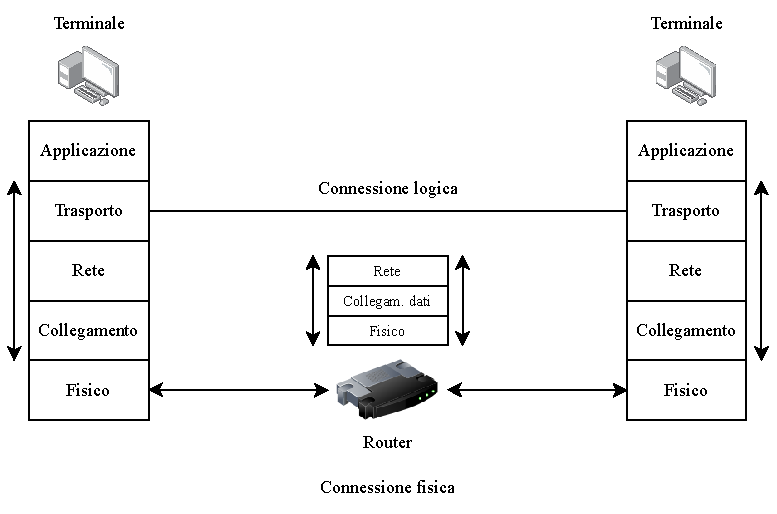
\includegraphics[width=\textwidth]{img/incapsulamento.pdf}
	\end{figure}

	La comunicazione avviene nel seguente modo:
	
	\begin{enumerate}
		\item Parte nel \textbf{\underline{livello di applicazione}} del host mittente il quale crea un \textbf{messaggio a livello di applicazione} (\emph{application-layer message}) concatenando informazioni aggiuntive, o meglio le informazioni di intestazione. Alla fine del processo di creazione, il messaggio viene passato al livello inferiore, quello di trasporto;
		
		\item A \textbf{\underline{livello di trasporto}} vengono aggiunte altre informazioni di intestazione. Le intestazioni di applicazione e trasporto formano il \textbf{segmento a livello di trasporto} (\emph{transport-layer segment}) che incapsula il messaggio a livello di applicazione. Infine, il livello di trasporto passa il messaggio al livello di rete;
		
		\item A \textbf{\underline{livello di rete}} vengono aggiunte informazioni come gli indirizzi dei sistemi periferici di sorgente e di destinazione. Facendo così viene creato un \textbf{datagramma a livello di rete} (\emph{network-layer datagram}). Infine, il messaggio viene passato al livello collegamento (\emph{link});
		
		\item A \textbf{\underline{livello di collegamento}} le informazioni aggiuntive creano un \textbf{frame a livello di collegamento} (\emph{link-layer frame});
		
		\item A \textbf{\underline{livello fisico}} vengono inviati i dati al router e qui termina l'incapsulamento.
	\end{enumerate}

	\noindent
	Per cui ad ogni livello, il pacchetto ha due tipi di campi: l’intestazione e \textbf{payload} (il carico utile trasportato). Il payload è tipicamente un pacchetto proveniente dal livello superiore.
	
	\section{Indirizzi IP}
	
	\subsection{Indirizzi IP}
	
	Un indirizzo IP consente di rendere \textbf{identificativo} e \textbf{univoco} un host all'interno della rete. Gli indirizzi IP vengono \textbf{rappresentati} con 32 bit e utilizzando una \textbf{notazione decimale puntata}. Prendendo in considerazione l’architettura di rete spiegata nel capitolo precedente, l’\underline{IP si posiziona al livello di rete}, nel quale viene aggiunto al messaggio da inviare.\newline
	
	\noindent
	La \textcolor{Red3}{\textbf{notazione decimale puntata}} è una rappresentazione degli indirizzi IP che facilita la lettura. Il modus operandi per ottenere tale notazione è il seguente:
	
	\begin{enumerate}
		\item Dividere i bit in 4 gruppi, ovvero 8 bit per ciascun gruppo;
		
		\item Traduzione di ogni gruppo da binario a decimale;
		
		\item Divisione di ogni gruppo da un punto.
	\end{enumerate}

	\noindent
	Negli indirizzi IP è importante dividere il prefisso dal suffisso poiché ogni parte ha un significato diverso:
	
	\begin{itemize}
		\item \textbf{\underline{Prefisso}}, identifica una rete all'interno di Internet;
		\item \textbf{\underline{Suffisso}}, identifica un host all'interno della rete.
	\end{itemize}
	
	\noindent
	Non esiste un numero specifico di indirizzi IP per il prefisso e per il suffisso. Questo perché dipendono entrambi dalla grandezza della rete; più è grande la rete e meno bit ha di prefisso.\newline
	
	\noindent
	Un \textbf{\emph{esempio}}: $157.27.12.63/16$, dove $157.27$ identifica il prefisso e $12.63$ il suffisso.
	
	\subsection{Maschera e blocco CIDR}
	
	Per identificare il numero di bit presenti nel prefisso, il calcolatore utilizza una sequenza di 32 bit in cui i bit del prefisso sono posti tutti a uno e i restanti a zero. Questo metodo si chiama maschera e un esempio di \textcolor{Red3}{\textbf{maschera}} 16 (notazione: /16):
	
	\begin{equation*}
		11111111111111110000000000000000
	\end{equation*}

	\noindent
	Che rappresenta l'indirizzo: $255.255.0.0$\newline
	
	\noindent
	Per cui si può affermare che la maschera \textbf{identifica} la grandezza della rete. Pensandoci, più è grande la maschera e più piccola è la rete visto che c’è una stretta relazione con il prefisso di un indirizzo IP.\newline
	
	\noindent
	Un \textcolor{Red3}{\textbf{blocco CIDR}} (\emph{Classless Inter-Domain Routing}) è un intervallo di indirizzi IP che sono disponibili nella propria rete.
	
	\newpage
	
	\subsection{\textcolor{Red3}{Esercizio di traduzione e numero host}}
	
	Dato il seguente indirizzo in notazione binaria:
	
	\begin{equation*}
		11100111 \hspace{1em} 11011011 \hspace{1em} 10001011 \hspace{1em} 01101111
	\end{equation*}

	\noindent
	Si rappresenta in notazione decimale puntata.\newline
	
	\noindent
	Per \textbf{prima cosa} si esegue la traduzione di ogni gruppo da binario a decimale:
	
	\begin{itemize}
		\item $11100111 \longrightarrow 2^{7} \cdot 1 + 2^{6} \cdot 1 + 2^{5} \cdot 1 + 2^{4} \cdot 0 + 2^{3} \cdot 0 + 2^{2} \cdot 1 + 2^{1} \cdot 1 + 2^{0} \cdot 1 = 231$
		
		\item $11011011 \longrightarrow 2^{7} \cdot 1 + 2^{6} \cdot 1 + 2^{5} \cdot 0 + 2^{4} \cdot 1 + 2^{3} \cdot 1 + 2^{2} \cdot 0 + 2^{1} \cdot 1 + 2^{0} \cdot 1 = 219$
		
		\item $10001011 \longrightarrow 2^{7} \cdot 1 + 2^{6} \cdot 0 + 2^{5} \cdot 0 + 2^{4} \cdot 0 + 2^{3} \cdot 1 + 2^{2} \cdot 0 + 2^{1} \cdot 1 + 2^{0} \cdot 1 = 139$
		
		\item $01101111 \longrightarrow 2^{7} \cdot 0 + 2^{6} \cdot 1 + 2^{5} \cdot 1 + 2^{4} \cdot 0 + 2^{3} \cdot 1 + 2^{2} \cdot 1 + 2^{1} \cdot 1 + 2^{0} \cdot 1 = 111$
	\end{itemize}

	\noindent
	E infine si riscrive la notazione in notazione decimale puntata:
	
	\begin{equation*}
		231.219.139.111
	\end{equation*}

	\noindent
	Adesso viene eseguita la conversione binaria della notazione decimale puntata del seguente indirizzo:
	
	\begin{equation*}
		221.34.255.82
	\end{equation*}

	\noindent
	Per \textbf{prima cosa} si esegue la traduzione di ogni gruppo. La traduzione non è banale, difatti si prenderà ciascun gruppo, si dividerà per due e nella colonna di destra verranno scritti i riporti. Infine, il numero binario sarà scritto dal numero di riporto del numero più basso, fino al numero più alto:
	
	\begin{center}
		\begin{tabular}{r|c}
			$221 \div 2$	&	1 \\
			$110 \div 2$	&	0 \\
			$55 \div 2$		&	1 \\
			$27 \div 2$		&	1 \\
			$13 \div 2$		&	1 \\
			$6 \div 2$		&	0 \\
			$3 \div 2$		&	1 \\
			$1 \div 2$		&	1			
		\end{tabular}
	\end{center}

	\noindent
	E così via. Unica accortezza da \textbf{ricordare} che se il numero di bit fosse meno di 8, si aggiungono zeri nella parte più significativa.\newline
	
	\noindent
	Dopo alcuni calcoli l’indirizzo IP in binario è:
	
	\begin{equation*}
		\binaryaddress{11011101}{00100010}{11111111}{01010010}
	\end{equation*}

	\noindent
	Una rete con un suffisso di /20, quanti host contiene? Dato un indirizzo IP da 32 bit, se il suffisso ha 20 bit, allora: $2^{32} \div 2^{20} = 2^{12}$. Una rete con un suffisso di 20 bit, avrà un prefisso di 12 bit, ovvero $2^{12} \longrightarrow 4096$ indirizzi.
	
	\newpage
	
	\section{Indirizzi IP privati}
	
	\subsection{Indirizzi IP privati}
	
	Gli indirizzi IP riservati sono indirizzi IP che non possono essere assegnati a nessun host. In particolare, sono:
	
	\begin{itemize}
		\item \textbf{Indirizzo di rete}: tutti i bit del suffisso sono posti a zero;
		\item \textbf{Indirizzo di Direct Broadcast}: tutti i bit del suffisso sono posti a uno;
		\item \textbf{Indirizzo con tutti i bit a zero};
		\item \textbf{Indirizzo con tutti i bit a uno};
	\end{itemize}

	\subsection{\textcolor{Red3}{Esercizio subnetting, creazione sottoreti partendo da un blocco di indirizzi}}
	
	La tecnica di \textcolor{Red3}{\textbf{\emph{subnetting}}} consiste nel suddividere una rete in più rete, chiamate sottoreti. L'esercizio fornisce un indirizzo IP:
	
	\begin{equation*}
		180.190.0.0/16
	\end{equation*}

	\noindent
	E l'obbiettivo è quello di creare due sottoreti di grandezza identica.\newline
	
	\noindent
	Per \textbf{prima cosa} si deve effettuare la conversione da notazione decimale puntata a notazione binaria:
	
	\begin{equation*}
		\binaryaddress{10110100}{10111110}{00000000}{00000000}
	\end{equation*}

	\noindent
	A questo punto è possibile creare due sottoreti come richiesto dall’esercizio.\newline
	
	\noindent
	Per farlo si identifica il primo bit utile nell'indirizzo binario. Esso è possibile trovarlo escludendo il prefisso ($/16$). Quindi, si conta dal bit più significativo $16$ bit, escluso sé stesso, arrivando al bit numero 17, ovvero il più significativo del terzo gruppo:
	
	\begin{equation*}
		\binaryaddress{10110100}{10111110}{\textcolor{Red3}{\boldsymbol{x}}0000000}{00000000}
	\end{equation*}

	\noindent
	Al posto della $\textcolor{Red3}{\boldsymbol{x}}$ verrà sostituito lo zero per creare la prima rete e l’uno per creare la seconda rete. Gli indirizzi saranno:
	
	\begin{equation*}
		\begin{array}{ll}
			\text{Ind. bin. della \textbf{prima rete}:} 	& \binaryaddress{10110100}{10111110}{\textcolor{Red3}{\boldsymbol{0}}0000000}{00000000} \\
			\text{Ind. bin. della \textbf{seconda rete}:} 	& \binaryaddress{10110100}{10111110}{\textcolor{Red3}{\boldsymbol{1}}0000000}{00000000}
		\end{array}
	\end{equation*}

	\noindent
	Il \textbf{prefisso} delle sottoreti sarà aumentato di un solo bit, per cui saranno $/17$.\newline
	
	\noindent
	La \textbf{traduzione in decimale} sarà:
	
	\begin{itemize}
		\item \textbf{Prima rete:} $180.190.0.0/17$
		\item \textbf{Seconda rete:} $180.190.128.0/17$
	\end{itemize}

	\noindent
	La \textbf{maschera} delle sottoreti sarà formata da $17$ bit posti a $1$ partendo dal più significativo:
	
	\begin{equation*}
		\binaryaddress{11111111}{11111111}{10000000}{00000000}
	\end{equation*}

	\noindent
	E la \textbf{traduzione della maschera} in notazione decimale puntata sarà:
	
	\begin{equation*}
		255.255.128.0
	\end{equation*}

	\noindent
	Infine, la \textbf{dimensione dei blocchi} di rete:
	
	\begin{equation*}
		\begin{array}{llll}
			\textbf{Pre-subnetting}:	&	2^{32} \div 2^{16} = 2^{16}	&	\longrightarrow	&	65'536 \text{ indirizzi} \\
			&&& \\
			\textbf{Post-subnetting}: 	&	2^{32} \div 2^{17} = 2^{15}	&	\longrightarrow	&	32'768 \text{ indirizzi}
		\end{array}
	\end{equation*}

	\newpage
	
	\section{Socket e protocolli a livello di trasporto: TCP e UDP}
	
	\subsection{Socket}
	
	I sistemi periferici collegati a Internet forniscono un'\textcolor{Red3}{\textbf{interfaccia socket}} (\emph{socket interface}), che specifica come un programma eseguito su un sistema periferico possa chiedere a Internet di recapitare dati a un programma eseguito su un altro sistema periferico.\newline
	
	\noindent
	\emph{In altre parole}, l’interfaccia socket è un insieme di regole che il programma mittente deve seguire in modo che i dati siano recapitati al programma di destinazione.\newline
	
	\noindent
	È importante anche sapere l’esistenza delle \textbf{API} (\emph{Application Programmin Interface}) tra l’applicazione e la rete, poiché l’interfaccia socket non è altro che un’interfaccia di programmazione con cui le applicazioni di rete vengono costruite.\newline
	
	\noindent
	Infine, esistono due tipi di processi:
	
	\begin{itemize}
		\item Il \textbf{client}, ovvero colui che avvia la comunicazione e ha un \underline{IP dinamico};
		\item Il \textbf{server}, ovvero colui che attende di essere contattato per iniziare la sessione e ha un \underline{IP statico}.
	\end{itemize}

	\newpage
	
	\subsection{Protocolli nel livello di trasporto}
	
	Dopo il livello applicativo, si trova il livello di trasporto. Esso può utilizzare due possibili \textbf{protocolli} nelle reti TCP/IP: \textcolor{Red3}{\textbf{TCP}} e \textcolor{Red3}{\textbf{UDP}}.
	
	\subsubsection{Protocollo TCP}\label{protocollo TCP}
	
	Il protocollo TCP prevede la fornitura di un servizio \textbf{orientato alla connessione} (\emph{Connection oriented communication}) e il \textbf{trasporto affidabile dei dati}.\newline
	
	\noindent
	Le \textbf{caratteristiche} di questo protocollo sono:
	
	\begin{itemize}
		\item \textcolor{Green4}{\textbf{Servizio orientato alla connessione}}. Questa caratteristica deriva dal fatto che vengono scambiate delle informazioni di controllo prima che i messaggi veri e propri vengano processati dal livello applicativo. Questo \underline{scambio di messaggi} prende il nome di \textbf{handshaking}.\newline
		Successivamente, \emph{se tutto è andato a buon fine}, si instaura una \textbf{connessione TCP} tra le socket dei due processi. La connessione viene chiamata \textbf{\emph{full-duplex}} ovvero i due processi possono scambiarsi i messaggi contemporaneamente sulla connessione.
		Infine, per \underline{terminare la connessione}, il mittente e il destinatario si \textbf{scambiano} alcuni \textbf{messaggi}.
		
		\item \textcolor{Green4}{\textbf{Servizio di trasferimento affidabile}}. Il protocollo è affidabile poiché i vari controlli effettuati permettono di:
		\begin{itemize}
			\item Non perdere dati;
			\item Inviarli nel giusto ordine;
			\item Evitare duplicazioni.
		\end{itemize}
	\end{itemize}
	
	\noindent
	Inoltre, questo protocollo implementa un meccanismo di \textbf{controllo della congestione}. Nel caso in cui si manifestasse, eseguirebbe una \dquotes{strozzatura} del processo d’invio.\newline
	
	\noindent
	Infine, il protocollo negli ultimi anni implementa anche il \textbf{\emph{secure sockets layer}} (\textbf{SSL}). Ovvero un servizio aggiuntivo che consente la cifratura dei messaggi. Attenzione che questo servizio deve essere attivo sia lato client che lato server, altrimenti si rischia che una delle due parti non possa decifrare il messaggio ricevuto.
	
	\newpage
		
	\subsubsection{Protocollo UDP}\label{protocollo UDP}
	
	Al contrario del protocollo TCP, UDP è un protocollo di trasporto \textbf{leggero}, \textbf{rapido} e \textbf{minimalista}. Esso \emph{\textbf{non}} necessita di connessione, per cui \underline{non esegue} \underline{alcun handshaking} e di conseguenza \textbf{non} fornisce neanche un \textbf{trasferimento dati affidabile}.\newline
	
	\noindent
	Per cui, quando processo invia un messaggio tramite un socket, UDP \textbf{non garantisce la consegna del messaggio}. Inoltre, i messaggi potrebbero giungere a destinazione non in ordine.\newline
	
	\noindent
	La \textbf{rapidità del protocollo} è dovuta anche al fatto che i pacchetti vengono inviati direttamente \textbf{senza} utilizzare un sistema di \textbf{controllo della congestione}. Tuttavia, il reale throughput end-to-end potrà essere inferiore a causa della banda limitata dei collegamenti coinvolti o a causa della congestione. Si ricorda che con il termine throughput ci si riferisce al tasso con quale il processo mittente può inviare i bit al processo ricevente.
	
	\begin{itemize}
		\item \textcolor{Green4}{\textbf{\underline{Vantaggi}}}
		\begin{itemize}
			\item \textbf{\underline{Leggero}} poiché non ha bisogno di controllare che la connessione sia instaurata, ovvero il fenomeno di \emph{handshaking} viene eliminato;
			
			\item \textbf{\underline{Rapido}} poiché non esiste nessun sistema di controllo della congestione, per cui i pacchetti vengono mandati uno dopo l'altro. Talvolta il throughput potrebbe essere minore a causa di eventuali colli di bottiglia;
			
			\item \textbf{\underline{Minimalista}} poiché non implementa tecniche particolari come detto in precedenza.
		\end{itemize}
		
		\item \textcolor{Red3}{\textbf{\underline{Svantaggi}}}
		\begin{itemize}
			\item \textbf{\underline{Nessuna affidabilità}} a causa della mancanza del fenomeno di \emph{handshaking}. Quindi, \textbf{nessuna garanzia di consegna} del messaggio;
			
			\item \textbf{\underline{Alta probabilità di congestione}} dovuta alla mancanza di controllo di essa. Quindi, il buffer potrebbe riempirsi rapidamente;
			
			\item \textbf{\underline{Messaggi non in ordine}}.
		\end{itemize}
	\end{itemize}

	\newpage
	
	\subsection{\textcolor{Red3}{Esercizio sull'indirizzamento}}
	
	Dato il seguente IP:
	
	\begin{equation*}
		140.120.84.20/20
	\end{equation*}
	
	\noindent
	Determinare l’indirizzo di rete.\newline
	
	\noindent
	Il \textbf{primo passo} è la traduzione dell’IP da notazione decimale puntata a notazione binaria:
	
	\begin{equation*}
		\begin{array}{lll}
			140_{10}	& \longrightarrow & 10001100 \\
			&& \\
			120_{10}	& \longrightarrow & 01111000 \\
			&& \\
			84_{10}		& \longrightarrow & 01010100 \\
			&& \\
			20_{10}		& \longrightarrow & 00010100
		\end{array}
	\end{equation*}
	
	\noindent
	Scrivendo l’indirizzo esteso:
	
	\begin{equation*}
		\binaryaddress{10001100}{01111000}{01010100}{00010100}
	\end{equation*}

	\noindent
	Il \textbf{secondo passo} è l’azzeramento del suffisso (bits in rosso) dato che l’indirizzo di rete ha il prefisso \emph{non} nullo e il suffisso con tutti i bit a zero. Il prefisso viene dato dall’ esercizio, ovvero $/20$:
	
	\begin{equation*}
		\binaryaddress{10001100}{01111000}{0101\textcolor{Red3}{\boldsymbol{0000}}}{\textcolor{Red3}{\boldsymbol{00000000}}}
	\end{equation*}

	\noindent
	Il \textbf{terzo} e ultimo \textbf{passo} è la conversione in decimale e scrivere l’indirizzo di rete in notazione decimale puntata:
	
	\begin{equation*}
		\begin{array}{lll}
			10001100_{2}	& \longrightarrow & 140_{10} \\
			&& \\
			01111000_{2}	& \longrightarrow & 120_{10} \\
			&& \\
			01010000_{2}	& \longrightarrow & 80_{10} \\
			&& \\
			00000000_{2}	& \longrightarrow & 0_{10}
		\end{array}
	\end{equation*}

	\noindent
	E l'indirizzo di rete sarà:
	
	\begin{equation*}
		140.120.80.0/20
	\end{equation*}

	\newpage
	
	\subsection{\textcolor{Red3}{Esercizio subnetting - Avanzato}}
	
	Date 3 reti LAN, viene assegnato il blocco di rete 165.5.1.0/24. Creare 3 sottoreti per ogni rete LAN in modo da avere lo stesso numero di host.\newline
	
	Il \textbf{primo passo} è la classica traduzione in binaria. Si deve tradurre l’indirizzo da notazione decimale puntata a binario:
	
	\begin{equation*}
		\begin{array}{lll}
			165_{10}	& \longrightarrow & 10100101_{2} \\
			5_{10}		& \longrightarrow & 00000101_{2} \\
			1_{10}		& \longrightarrow & 00000001_{2} \\
			0_{10}		& \longrightarrow & 00000000_{2}
		\end{array}
	\end{equation*}

	\noindent
	Il \textbf{secondo passo} è quello di creare delle sottoreti. Per farlo si deve prendere in considerazione il suffisso. Prima di tutto, si scrive l’indirizzo in notazione binaria:
	
	\begin{equation*}
		\binaryaddress{10100101}{00000101}{00000001}{00000000}
	\end{equation*}

	\noindent
	La creazione di 3 sottoreti prevede almeno due bit. Difatti, se venisse scelto un bit, si potrebbe creare al massimo 2 sottoreti. Per cui, dall’indirizzo in notazione binaria, si riservano (x in rosso) due bit nel suffisso per creare le sottoreti:
	
	\begin{equation*}
		\binaryaddress{10100101}{00000101}{00000001}{\textcolor{Red3}{\boldsymbol{xx}}000000}
	\end{equation*}

	\noindent
	Riservando questi due bit, adesso si sono create quattro sottoreti:
	
	\begin{equation*}
		\begin{array}{ll}
			\textbf{LAN1.} & \binaryaddress{10100101}{00000101}{00000001}{\textcolor{Red3}{\boldsymbol{00}}000000} \\
			\textbf{LAN2.} & \binaryaddress{10100101}{00000101}{00000001}{\textcolor{Red3}{\boldsymbol{01}}000000} \\
			\textbf{LAN3.} & \binaryaddress{10100101}{00000101}{00000001}{\textcolor{Red3}{\boldsymbol{10}}000000} \\
			\textbf{LAN4.} & \binaryaddress{10100101}{00000101}{00000001}{\textcolor{Red3}{\boldsymbol{11}}000000} \\
		\end{array}
	\end{equation*}

	\noindent
	La prima sottorete è assegnata alla LAN1, la seconda alla LAN2, la terza alla LAN3 e la quarta è considerata libera. Essa potrà essere utilizzata in futuro.\newline
	
	\noindent
	Il \textbf{terzo passo} è calcolare il nuovo prefisso delle sottoreti. Ogni sottorete è formata dal prefisso della rete originaria ($/24$), più due bit che sono serviti per creare le 3 reti. Quindi, il nuovo prefisso delle 3 reti è diventato $/26$.\newline
	
	\noindent
	Infine, il \textbf{quarto passo} è la scrittura in notazione decimale puntata delle tre reti e il calcolo degli indirizzi disponibili.\newline
	
	\noindent
	La conversione è semplice e si omettono i passaggi e le spiegazioni:
	
	\begin{equation*}
		\begin{array}{ll}
			\textbf{LAN1.} & 165.5.1.0/26 \\
			\textbf{LAN2.} & 165.5.1.64/26 \\
			\textbf{LAN3.} & 165.5.1.128/26 \\
			\textbf{LAN4.} & 165.5.1.192/26 \\
		\end{array}
	\end{equation*}

	\noindent
	E la rete è passata da avere ($2^{32} \div 2^{24} = 2^{8}$) 256 indirizzi disponibili a ($2^{32} \div 2^{26} = 2^{6}$) 64 indirizzi.
	
	\newpage
	
	\subsubsection{\textcolor{Red3}{Domanda bonus}}
	
	Se la LAN1 avesse dovuto avere il doppio degli indirizzi rispetto alla LAN2 e alla LAN3, l'esercizio come si sarebbe svolto?\newline
	
	\noindent
	In questo caso specifico, partendo dal \textbf{passo numero due}, ovvero alla creazione delle sottoreti, si sarebbe proceduti in maniera diversa.\newline
	
	\noindent
	Invece di prendere due bit, si prende un solo bit che ci permette di creare due sottoreti: nella prima sottorete si assegna la LAN1 e nella seconda sottorete si assegnano LAN2 e LAN3.
	\begin{equation*}
		\binaryaddress{10100101}{00000101}{00000001}{\textcolor{Red3}{\boldsymbol{x}}0000000}
	\end{equation*}
	
	\noindent
	Creando le due sottoreti:
	\begin{gather*}
		\binaryaddress{10100101}{00000101}{00000001}{\textcolor{Red3}{\boldsymbol{0}}0000000} \\
		\binaryaddress{10100101}{00000101}{00000001}{\textcolor{Red3}{\boldsymbol{1}}0000000}
	\end{gather*}
	
	\noindent
	Il \textbf{terzo passo} è quello di creare le due sottoreti all’interno del secondo indirizzo. Due sottoreti necessitano di due bit, per cui la divisione sarà:
	\begin{equation*}
		\begin{array}{ll}
			\textbf{LAN2.} & \binaryaddress{10100101}{00000101}{00000001}{1\textcolor{Red3}{\boldsymbol{0}}000000} \\
			\textbf{LAN3.} & \binaryaddress{10100101}{00000101}{00000001}{1\textcolor{Red3}{\boldsymbol{1}}000000}
		\end{array}
	\end{equation*}

	\noindent
	Infine, il \textbf{quarto passo} è quello di calcolare la maschera delle reti, riscrivere gli indirizzi in notazione decimale puntata e calcolare il numero di indirizzi possibili.\newline
	
	\noindent
	La maschera per la LAN1 è aumentata di 1 dalla rete di partenza, per cui $/25$. Mentre per la LAN2 e LAN3 è aumentata di 2 bit, ovvero $/26$.\newline
	
	\noindent
	La scrittura in notazione decimale puntata sarà:
	\begin{equation*}
		\begin{array}{ll}
			\textbf{LAN1.} & 165.5.1.0/25 \\
			\textbf{LAN2.} & 165.1.128/26 \\
			\textbf{LAN3.} & 165.1.192/26
		\end{array}
	\end{equation*}

	\noindent
	E il numero di indirizzi della LAN1 saranno ($2^{32} \div 2^{25} = 2^{7}$) 128, mentre quelli della LAN2 e della LAN3 rimarranno a 64 indirizzi.
	
	\newpage
	
	\section{Protocollo HTTP}
	
	\subsection{Protocollo HTTP}
	
	\textcolor{Red3}{\textbf{HTTP}} (\emph{Hypertext Transfer Protocol}), protocollo a livello di applicazione del Web, costituisce il cuore del Web. Questo \textbf{protocollo} è implementato nei programmi in esecuzione su sistemi periferici diversi che comunicano tra loro scambiandosi messaggi HTTP.\newline
	
	\noindent
	Una \textbf{pagina web} (\emph{web page}), detta anche documento, è costituita da oggetti. Un \textbf{oggetto} è semplicemente un file indirizzabile tramite un URL. La maggioranza delle pagine web consiste di un \textbf{file HTML principale} e diversi oggetti referenziati da esso.\newline
	
	\noindent
	Un \textbf{browser web} implementa il lato \emph{client} di HTTP, ovvero l’utente stesso. Mentre il \textbf{web server} implementa il lato server di HTTP, ospita oggetti web, indirizzabili tramite URL.\newline
	
	\noindent
	HTTP utilizza il protocollo \textbf{TCP come protocollo di trasporto}. Il client HTTP per prima cosa inizia una connessione TCP con il server. Una volta stabilita, i processi client e server accedono a TCP attraverso le proprie socket.\newline
	
	\noindent
	Dato che i server HTTP non mantengono informazioni sui client, HTTP è classificato come \textbf{protocollo senza memoria di stato} (\emph{stateless protocol}). Un \textbf{web server} è \textbf{sempre attivo}, ha un indirizzo IP fisso e risponde potenzialmente alle richieste provenienti da milioni di diversi browser.
	
	\subsection{HTTP con connessioni (non) persistenti}
	
	Sia i client che i server possono avere due diverse configurazioni: le connessioni persistenti e le connessioni non persistenti. Prima di iniziare la spiegazione, si introduce il concetto di \textcolor{Red3}{\textbf{round-trip time}} (\textbf{RTT}), che rappresenta il \textbf{tempo impiegato da un pacchetto per viaggiare dal client al server e poi tornare al client}. Esso include i \textbf{ritardi di propagazione}, di \textbf{accodamento} nei \textbf{router} e nei \textbf{commutatori intermedi} nonché di elaborazione del pacchetto.
	
	\newpage
	
	\subsubsection{Connessioni non persistenti}
	
	Per spiegare le connessioni non persistenti, si faccia riferimento ad un esempio in cui c’è il trasferimento di una pagina web dal server al client. Si supponga che la pagina consista di un file HTML principale e di 10 immagini, e tutti gli oggetti risiedano sullo stesso server.
	
	\begin{enumerate}
		\item Il processo client HTTP inizializza una connessione di tipo TCP con il server sulla porta 80, ovvero la porta di default per HTTP.
		
		\item Il client HTTP, tramite la socket, invia al server un messaggio di richiesta del file principale.
		
		\item Il processo server HTTP riceve il messaggio di richiesta attraverso la socket, recupera l’oggetto richiesto dalla propria memoria, lo incapsula in un messaggio di risposta che viene inviato al client attraverso la socket.
		
		\item Il processo server HTTP comunica a TCP di concludere la connessione. Tuttavia, il protocollo TCP garantisce la consegna del messaggio, per cui non termina la connessione finché il client non ha ricevuto l’intero messaggio.
		
		\item Il client HTTP riceve il messaggio di risposta. La connessione TCP termina a questo punto e il messaggio ricevuto indica che l’oggetto incapsulato è un file HTML. Il client estrae il file del messaggio di risposta, esamina il file HTML e trova i riferimenti ai 10 oggetti.
		
		\item Infine, vengono ripetuti tutti i primi quattro passi per ciascuno degli oggetti referenziati.
	\end{enumerate}

	\noindent
	Si conclude che l’utilizzo di connessione non persistenti, consente di chiudere ogni connessione aperta dopo l’invio dell’oggetto da parte del server e dopo aver ricevuto una conferma dal client.\newline
	
	\noindent
	Nell’esempio vengono create 11 connessioni TCP, una per ogni oggetto richiesto.\newline
	
	\noindent
	Come si può notare, queste connessioni presentano alcuni \textbf{limiti}:
	
	\begin{enumerate}
		\item Per ogni oggetto richiesto occorre stabilire e mantenere una nuova connessione.
		
		\item Per ogni connessione si deve allocare buffer e mantenere variabili TCP sia nel client che nel server.
		
		\item Ciascun oggetto subisce un ritardo di consegna di due RTT: uno per stabilire la connessione TCP e uno per richiedere e ricevere un oggetto.
	\end{enumerate}

	\noindent
	Questi limiti richiedono un grande onere sul web server che deve aprire nuove connessioni ogni qualvolta ci deve essere uno scambio di dati. Il grande onere riguarda soprattutto il momento in cui il server riceve centinaia di richieste da parte dei client.
	
	\newpage
	
	\subsubsection{Connessioni persistenti}
	
	La particolarità delle connessioni persistenti è la possibilità da parte del server di lasciare aperta la connessione TCP dopo l’invio di una risposta. Così facendo, le richieste/risposte future da parte degli stessi client e server potranno essere trasmesse sulla stessa connessione.\newline
	
	\noindent
	Difatti, il server può inviare un’intera pagina web \textbf{sfruttando} solamente \textbf{una connessione} TCP permanente, oppure inviare più pagine web allo stesso client.\newline
	
	\noindent
	Le \textbf{richieste} possono essere effettuate \textbf{una dopo l’altra senza attendere} le risposte delle eventuali richieste pendenti (\emph{pipelining}).\newline
	
	\noindent
	In generale, il server HTTP \textbf{chiude la connessione} quando essa rimane inattiva per un lasso di tempo arbitrario.
	
	\newpage
	
	\subsection{Formato dei messaggi HTTP}
	
	Esistono due tipi di formati di questo protocollo: il messaggio di richiesta HTTP e messaggio di risposta HTTP.
	
	\subsubsection{Messaggio di richiesta HTTP}
	
	I messaggi di richiesta possono avere un numero indefinito di righe, anche una sola.\newline
	
	\noindent
	Ogni riga alla fine ha un \textbf{carattere di ritorno a capo} (\emph{carriage return}) e un \textbf{carattere di nuova linea} (\emph{line feed}).\newline
	
	\noindent
	L’ultima riga è seguita da una coppia di caratteri di ritorno a capo e nuova linea aggiuntivi.\newline
	
	\noindent
	In generale, la \textbf{prima riga} è la \textbf{riga di richiesta} (\emph{request line}) e quelle successive si chiamano \textbf{righe di intestazione} (\emph{header lines}).\newline
	
	\noindent
	La \textbf{riga di richiesta} è formata da tre campi:
	
	\begin{itemize}
		\item Campo \textbf{metodo} (GET, POST, HEAD, PUT, DELETE)
		\item Campo \textbf{URL}
		\item Campo \textbf{versione HTTP}
	\end{itemize}
	
	\noindent
	Le \textbf{righe di intestazione} possono essere di molti tipi. La riga \textbf{Host} specifica l’host su cui risiede l’oggetto, la riga \textbf{Connection} indica se il server deve effettuare una connessione di tipo persistente o non persistente, la riga \textbf{User-agent} specifica il tipo di browser che sta effettuando la richiesta al server e, infine, la riga \textbf{Accept-language} indica se l’utente preferisce ricevere una versione dell’oggetto nella lingua specificata; in caso di mancanza, il server provvederà a fornire la versione di default.
	
	\newpage
	
	\subsubsection{Messaggio di risposta HTTP}
	
	Nei messaggi di risposta ci sono tre sezioni importanti: una \textbf{riga di stato iniziale}, le \textbf{righe di intestazione} e il \textbf{corpo}.\newline
	
	\noindent
	La \textbf{riga di stato iniziale} presenta tre campi:
	
	\begin{itemize}
		\item \textbf{Versione del protocollo}
		\item \textbf{Codice di stato}
		\item \textbf{Messaggio di stato} (approfondimento alla fine di questo paragrafo)
	\end{itemize}

	\noindent
	Le \textbf{righe di intestazione} possono essere di tipo \textbf{Connection} per comunicare al client la gestione della connessione, per esempio “Connection: close” per indicare l’intenzione di chiudere la connessione TCP dopo l’invio del messaggio; di tipo \textbf{Date} per indicare l’ora e la data di creazione e invio, da parte del server, della risposta HTTP; di tipo \textbf{Server} per indicare che il messaggio è stato generato da un determinato tipo di web server, simile alla riga “User-agent” nel messaggio di richiesta; di tipo \textbf{Last-Modified} per indicare l’istante e la data in cui l’oggetto è stato creato o modificato per l’ultima volta; di tipo \textbf{Content-Length} per indicare il numero di byte dell’oggetto inviato; di tipo \textbf{Content-Type} per indicare il tipo di oggetto specificato nel corpo.\newline
	
	\noindent
	Le \textbf{righe di corpo} sono il fulcro del messaggio. Esse contengono l’oggetto richiesto.\newline
	
	\noindent
	Nella \textbf{riga di stato iniziale}, i due campi \textbf{codice} e \textbf{messaggio di stato} indicano operazioni importanti. Qui di seguito si elencano i codici con i relativi messaggi, sono riportati solo i più importanti:
	
	\begin{itemize}
		\item 200 OK: la richiesta ha avuto successo e in risposta si invia l'informazione.
		
		\item 301 Moved Permanently: l’oggetto richiesto è stato trasferito in modo permanente; il nuovo URL viene specificato nell’intestazione, campo Location, del messaggio di risposta.
		
		\item 400 Bad Request: codice di errore generico che indica che la richiesta non è stata compresa dal server.
		
		\item 404 Not Found: il documento richiesto non esiste sul server.
		
		\item 505 HTTP Version Not Supported: il server non dispone della versione di protocollo HTTP richiesta.
	\end{itemize}

	\newpage
	
	\subsection{Cookie}
	
	I \textcolor{Red3}{\textbf{\emph{cookie}}} è un meccanismo utilizzato dal server per sapere se ha interagito precedentemente con un determinato client.\newline
	
	\noindent
	La \textbf{prima volta} che il \emph{client} interagisce con un \emph{server}, inviando una richiesta GET, il server crea un identificativo (codice) associato all'utente (e.g. 1234).\newline
	
	\noindent
	Il server \textbf{risponde} con una richiesta REPLY HTTP, impostando nell'intestazione il valore \emph{\textbf{set-cookie}} al valore impostato al passaggio prima. Alla ricezione della risposta, il \emph{client} memorizza l'indirizzo della pagina usato per fare la prima richiesta GET e il codice fornito dal server (\emph{set-cookie}).\newline
	
	\noindent
	\textbf{Dopo una serie di interazioni}, quando il \emph{client} effettuerà di nuovo una richiesta GET al server specifico, esso dovrà indicare come codice \emph{cookie}, il codice salvato la prima volta. Invece, il server controllerà la storia associata all'utente con il codice fornito e restituisce una risposta specifica all'utente.
	
	\subsection{Cache di rete}
	
	La \textcolor{Red3}{\textbf{cache di rete}} intercetta i messaggi e memorizza le risposte. I vantaggi riguardano principalmente la velocità. Il suo funzionamento è il seguente:
	
	\begin{enumerate}
		\item Invio della richiesta di un determinato dato da parte del \emph{client};
		
		\item \textbf{Cache di rete} intercetta il messaggio e controlla se ha il dato richiesto:
		\begin{itemize}
			\item Se il \textbf{dato è presente}:
			\begin{enumerate}
				\item La cache di rete invia una richiesta di tipo \textcolor{Red3}{\textbf{GET condizionale}} per verificare che il contenuto del dato richiesto non sia stato modificato nel server (campo nell'intestazione: \emph{if-modified-since});
				
				\item Il server risponde inviando un messaggio con scritto nell'intestazione \emph{not modified};
				
				\item Cache di rete invia direttamente il dato al client diminuendo il tempo d'attesa del mittente (lo scambio di messaggi piccoli tra cache di rete e server è rapido!).
			\end{enumerate}
		
			\item Se il \textbf{dato \underline{non} è presente}:
			\begin{enumerate}
				\item La cache di rete invia una richiesta di tipo \textcolor{Red3}{\textbf{GET condizionale}} per verificare che il contenuto del dato richiesto non sia stato modificato nel server (campo nell'intestazione: \emph{if-modified-since});
				
				\item Il server di destinazione risponde inviando i dati richiesti (operazione lenta);
				
				\item La cache di rete intercetta la risposta salvando una copia dei dati al suo interno. La risposta non viene bloccata, quindi arriva anche al client,
			\end{enumerate}
		\end{itemize}
	\end{enumerate}

	\newpage
	
	\section{DNS}
	
	\subsection{DNS}
	
	Gli host Internet possono essere identificati in vari modi. I \textbf{nomi degli host} (\emph{hostname}), per esempio \textsf{www.facebook.com} o \textsf{www.google.com}, risultano abbastanza appropriati per l’uomo, ma forniscono ben poca informazione sulla loro collocazione all’interno di Internet. Per cui, i nomi vengono utilizzati dagli utenti finali, mentre i calcolatori utilizzando gli \textbf{indirizzi IP} degli host.\newline
	
	\noindent
	Gli utenti finali inseriscono i nomi degli host e il calcolatore riesce a ottenere l’indirizzo IP grazie ad un servizio in grado di tradurre i nomi in indirizzi IP. Il suo nome è \textcolor{Red3}{\textbf{Domain Name System}} (DNS).\newline
	
	\noindent
	Il \textbf{DNS} è un \textbf{database} distribuito implementato in una \textbf{gerarchia} di \textbf{DNS server} e un protocollo a livello di applicazione che consente agli \textbf{host} di \textbf{interrogare} il \textbf{database}. Generalmente i DNS server sono macchine UNIX che eseguono un software chiamato BIND (\emph{Berkeley Internet name domain}). Il protocollo DNS utilizza \textbf{UDP} e la \textbf{porta 53}.\newline
	
	\noindent
	Nel dettaglio quello che succede nel momento in cui un utente digita un host name:
	
	\begin{enumerate}
		\item La macchina utente (\emph{client}) esegue l’applicazione DNS;

		\item Il browser estrae il nome del host dall’URL inserito e lo passa all’applicazione DNS;

		\item L’applicazione DNS esegue una interrogazione (\emph{query}), sul database di una DNS server, contenente l’hostname;

		\item L’applicazione DNS prima o poi riceve una risposta che include l’indirizzo IP corrispondente al host dell’hostname fornito;

		\item Una volta ricevuto l’indirizzo IP dal DNS, il browser può dare inizio a una connessione di tipo TCP verso il processo server HTTP collegato alla porta 80 di quell’indirizzo IP.
	\end{enumerate}

	\newpage
	
	\subsection{Approfondimento sul database distribuito e gerarchico}
	
	Il DNS utilizza un grande numero di server, organizzati in maniera gerarchica e distribuiti nel mondo. Nessun DNS server ha le corrispondenze per tutti gli host in Internet, che sono invece distribuite tra tutti i DNS server.\newline
	
	\noindent
	Esistono \textbf{tre classi} di DNS server:
	
	\begin{itemize}
		\item \textbf{Root server}. In Internet esistono 400 root server circa, dislocati in tutto il mondo. Essi sono gestiti da 13 diverse organizzazioni.\newline
		I root server forniscono gli indirizzi IP dei server TLD.
		
		\item \textbf{Top-level domain (TLD) server}. Questi server si occupano dei domini di primo livello quali \emph{com}, \emph{org}, \emph{net}, \emph{edu} e \emph{gov}, e di tutti i domini di primo livello relativi ai vari paesi, come \emph{uk}, \emph{fr}, \emph{ca} e \emph{jp}. Per esempio, l’azienda “Verisign Global Registry Services” gestisce i TLD server per il dominio com.\newline
		I server TLD forniscono gli indirizzi IP dei server autoritativi.
		
		\item \textbf{Server autoritativi}.	Ogni organizzazione dotata di host pubblicamente accessibili tramite Internet (quali web server e e-mail server) deve fornire record DNS pubblicamente accessibili che associno i nomi di tali host a indirizzi IP. Il DNS server autoritativo dell’organizzazione ospita questi record.\newline
		Un’organizzazione può scegliere di implementare il proprio server autoritativo oppure di pagare un fornitore di servizi per ospitare questi record su un suo server.
	\end{itemize}

	\noindent
	Un \textbf{esempio} riepilogativo può essere del tipo: si supponga che un client DNS voglia determinare l’indirizzo IP relativo all’hostname \textsf{www.amazon.com}.\newline
	Per fare ciò, il client dapprima contatta uno dei root server che gli restituisce uno o più indirizzi IP relativi al server TLD per il dominio \emph{com} (dominio gestito dall’azienda Verisign Global Registry Services).\newline
	Per cui, contatta uno di questi server TLD che gli restituisce uno o più indirizzi IP del server autoritativo per \textsf{amazon.com}.\newline
	Infine, contatta uno dei server autoritativi per \textsf{amazon.com} che gli restituisce l’indirizzo IP dell’hostname \textsf{www.amazon.com}.
	
	\newpage
	
	\subsection{\textcolor{Red3}{Esercizio - Determinare CIDR e creare subnetting con condizioni}}
	
	Si consideri la seguente rete formata da 5 sottoreti. Due indirizzi sono già assegnati alla rete:
	
	\begin{equation*}
		101.75.79.255 \hspace{3em} 101.75.80.0
	\end{equation*}

	\noindent
	Determinare il blocco CIDR più piccolo che contiene tali indirizzi. Per “più piccolo” si intende con numero minore di indirizzi.\newline
	
	\noindent
	Una volta trovato il blocco CIDR, creare 5 sottoreti con i seguenti vincoli:
	
	\begin{itemize}
		\item LAN1: Deve avere un prefisso di /21
		\item LAN2: Deve ospitare fino a 1000 host
		\item LAN3: Deve avere un prefisso di /23
		\item LAN4: Deve ospitare fino a 400 host
		\item LAN5: Deve avere la metà degli indirizzi a disposizione del blocco di partenza
	\end{itemize}

	\noindent
	Inizialmente si traducono gli indirizzi che si hanno in binario:
	\begin{equation*}
		\begin{array}{lll}
			101.75.79.255	& \longrightarrow & \binaryaddresspointed{01100101}{01000011}{01001111}{11111111} \\
			101.75.80.0		& \longrightarrow & \binaryaddresspointed{01100101}{01000011}{01010000}{00000000}
		\end{array}
	\end{equation*}

	\noindent
	Per \textbf{calcolare il prefisso} basta prendere in considerazione i bit identici nei due indirizzi. Il conteggio prosegue finché non si trova un bit che differisce. Per cui, in questo esercizio il bit numero 20 differisce, infatti nel primo indirizzo è 0, mentre nel secondo è 1. In conclusione, il prefisso è $/19$. Ponendo i restanti ($2^{32} \div 2^{19} = 2^{13}$) 13 bit a zero, si ottiene l’indirizzo di rete:
	\begin{equation*}
		101.75.64.0/19
	\end{equation*}
	Che avrà a disposizione $2^{13}$ indirizzi, ovvero 8192 il quale rappresenta il \textbf{blocco CIDR}.\newline
	
	\noindent
	Adesso inizia il calcolo dei vari indirizzi delle LAN. La LAN numero 5 deve avere la metà degli indirizzi disponibili messi a disposizione dalla rete di partenza, ovvero quella appena trovata. Per cui si creano le prime sottoreti (\emph{subnetting}) assegnandone una alla LAN5 che avrà per cui il prefisso maggiorato di un bit e un numero di indirizzi disponibili pari a: $2^{32} \div 2^{20} = 2^{12} \rightarrow 4096$.\newline
	
	\noindent
	Quindi si creano le due sottoreti:
	\begin{equation*}
		\begin{array}{lll}
			\binaryaddresspointed{01100101}{01000011}{010\textcolor{Red3}{\boldsymbol{0}}0000}{00000000} & \longrightarrow & 101.75.64.0/20 \\
			\binaryaddresspointed{01100101}{01000011}{010\textcolor{Red3}{\boldsymbol{1}}0000}{00000000} & \longrightarrow & 101.75.80.0/20
		\end{array}
	\end{equation*}
	E si afferma che l’indirizzo $101.75.64.0/20$ è assegnato alla LAN5.\newline
	
	\noindent
	Dal secondo indirizzo si creano altre sottoreti per soddisfare il criterio della prima LAN:
	\begin{equation*}
		\begin{array}{lll}
			\binaryaddresspointed{01100101}{01000011}{0101\textcolor{Red3}{\boldsymbol{0}}000}{00000000} & \longrightarrow & 101.75.80.0/21 \\
			\binaryaddresspointed{01100101}{01000011}{0101\textcolor{Red3}{\boldsymbol{1}}000}{00000000} & \longrightarrow & 101.75.88.0/21
		\end{array}
	\end{equation*}
	E si afferma che l’indirizzo $101.75.80.0/21$ è assegnato alla LAN1.\newline
	
	\noindent
	A questo punto si può notare che la seconda LAN richiede almeno 1000 host. Per soddisfare questa richiesta si può fare un calcolo rapido e confermare il fatto che se venissero create altre sottoreti dall’indirizzo disponibile qui sopra ($101.75.88.0/21$), si verrebbe a creare una rete con un prefisso di 22, un suffisso di $32-22=10$ bit, ovvero $2^{10} = 1024$ indirizzi. Quindi:
	\begin{equation*}
		\begin{array}{lll}
			\binaryaddresspointed{01100101}{01000011}{01011\textcolor{Red3}{\boldsymbol{0}}00}{00000000} & \longrightarrow & 101.75.88.0/22 \\
			\binaryaddresspointed{01100101}{01000011}{01011\textcolor{Red3}{\boldsymbol{1}}00}{00000000} & \longrightarrow & 101.75.92.0/22
		\end{array}
	\end{equation*}
	E si afferma che l’indirizzo $101.75.88.0/22$ è assegnato alla LAN2.\newline
	
	\noindent
	Infine, costruendo altre due sottoreti dall’indirizzo disponibile si troverebbe il nuovo indirizzo disponibile per la rete LAN numero 3 e 4. La numero 3 sarebbe rispettata perché il prefisso passerebbe da 22 a 23, mentre la numero 4 avrebbe $32-23=9$ bit di suffisso, ovvero $2^{9}=512$ indirizzi disponibili.\newline
	Per concludere quindi:
	\begin{equation*}
		\begin{array}{lll}
			\binaryaddresspointed{01100101}{01000011}{010111\textcolor{Red3}{\boldsymbol{0}}0}{00000000} & \longrightarrow & 101.75.92.0/23 \\
			\binaryaddresspointed{01100101}{01000011}{010111\textcolor{Red3}{\boldsymbol{1}}0}{00000000} & \longrightarrow & 101.75.94.0/23
		\end{array}
	\end{equation*}
	E si afferma che l’indirizzo $101.75.92.0/23$ è assegnato alla LAN3, mentre l’indirizzo $101.75.94.0/23$ è assegnato alla LAN4.
	
	\newpage
	
	\section{Posta elettronica SMTP e livello di trasporto}
	
	\subsection{Posta elettronica}
	
	L’e-mail rappresenta un mezzo di comunicazione asincrono: le persone inviano e leggono messaggi nel momento per loro più opportuno, senza doversi coordinare con altri utenti. I grandi vantaggi della posta elettronica sono la velocità, la facilità di distribuzione e il prezzo, ovvero gratuito.\newline
	
	\noindent
	In questo argomento ci sono tre \textbf{componenti principali}:
	\begin{enumerate}
		\item \textbf{User agent} (o agenti utente) che sono per esempio Microsoft Outlook e Apple Mail, i quali consentono agli utenti di leggere, rispondere, inoltrare, salvare e comporre i messaggi.
		
		\item \textbf{Server di posta} (o \emph{mail server}) costituiscono la parte centrale dell’infrastruttura del servizio di posta elettronica. Ciascun destinatario ha una \textbf{casella di posta} (\emph{mailbox}) collocata in un mail server.\newline
		Può capitare che una volta inviato il messaggio, il server non possa consegnare la posta. In tal caso esso la trattiene in una \textbf{coda di messaggi} e cerca di trasferirla in un secondo momento. In caso di mancata consegna dopo alcuni giorni dall’invio del messaggio, il server rimuove il messaggio e avvisa il mittente con un messaggio di posta elettronica.
		
		\item \textbf{Protocollo SMTP} (\emph{Simple Mail Transfer Protocol}) rappresenta il principale protocollo a livello di applicazione per la posta elettronica su Internet. Utilizza TCP, quindi viene considerato un servizio di trasferimento dati affidabile.\newline
		Questo protocollo viene eseguito sia lato client, quando è in esecuzione sul server di posta del mittente, sia lato server, quando è in esecuzione sul server del destinatario.
	\end{enumerate}

	\newpage

	\subsection{Protocollo SMTP}
	
	Il \textcolor{Red3}{\textbf{protocollo SMTP}} si occupa di \textbf{trasferire i messaggi dal mail server del mittente a quello del destinatario}. Nonostante la sua fama, SMTP rappresenta una tecnologia ereditata con caratteristiche \dquotes{arcaiche}.\newline
	\textbf{Per esempio}, il corpo dei messaggi di posta li tratta come semplice codice ASCII a 7 bit. Questa restrizione aveva senso nei primi anni '80, quando la capacità trasmissiva era scarsa e nessuno inviava per posta elettronica grandi allegati quali immagini, audio o video, ma oggi la restrizione all’ASCII a 7 bit è piuttosto penalizzante, in quanto richiede che i dati multimediali binari vengano codificati in ASCII prima di essere inviati e che il messaggio venga nuovamente decodificato in binario dopo il trasporto.\newline
	
	\noindent
	Il protocollo SMTP è uno dei protagonisti principali nella comunicazione tra client e server. Per esempio, supponiamo che Alice voglia inviare a Bob un semplice messaggio ASCII:
	\begin{enumerate}
		\item Alice invoca il proprio \emph{user agent} per la posta elettronica, fornisce l’indirizzo di posta di Bob, compone il messaggio e dà istruzione allo \emph{user agent} di inviarlo.
		
		\item Lo \emph{user agent} di Alice invia il messaggio al suo \emph{mail server}, il quale colloca esso in una coda di messaggi.
		
		\item Il lato client di SMTP, eseguito sul server del mittente (Alice), vede il messaggio nella coda dei messaggi e apre una connessione TCP verso un server SMTP in esecuzione sul \emph{mail server} del destinatario (Bob).
		
		\item Dopo un \emph{handshaking} SMTP, il client SMTP invia il messaggio di Alice sulla connessione TCP.
		
		\item Il \emph{mail server} di Bob, il lato server di SMTP riceve il messaggio, che viene posizionato nel \emph{mail server} della casella postale di Bob.
		
		\item Bob, quando ritiene opportuno, invoca il proprio user agent per leggere il messaggio.
	\end{enumerate}
	Si noti che solitamente SMTP non usa \emph{mail server} intermedi. Ovvero, se il server del mittente si trova a Hong Kong e quello del destinatario a St. Louis, la connessione TCP ha luogo direttamente tra le due città. In particolare, se il \emph{mail server} del destinatario è spento, il messaggio rimane nel \emph{mail server} del mittente e attende un nuovo tentativo. Questo è il significato dell’affermazione \textbf{\dquotes{il messaggio non viene posizionato in alcun \emph{mail server} intermedio}}.\newline
	
	\noindent
	Nell’esempio si è visto come il \emph{client} SMTP (in esecuzione sul \emph{mail server} del mittente) fa stabilire a TCP una \textbf{connessione sulla porta 25} verso il server SMTP (in esecuzione sul \emph{mail server} del destinatario).\newline
	Una volta stabilita la connessione, il \emph{server} e il \emph{client} effettuano una qualche forma di \emph{handshaking} a livello applicativo, ovvero il \emph{client} inizialmente invia prima l’e-mail del mittente e solo dopo aver ricevuto un messaggio di avvenuta ricezione invia il secondo messaggio contenente l’e-mail del destinatario.\newline
	Dopo l’\emph{handshaking}, il \emph{client} invia il messaggio e ripete il processo sulla stessa connessione TCP se ha altri messaggi da inviare al \emph{server}, altrimenti ordina a TCP di chiudere la connessione.
	
	\subsection{Livello di trasporto}
	
	\subsubsection{Definizione}
	
	Un \textcolor{Red3}{\textbf{protocollo a livello}} di trasporto mette a disposizione una \textbf{comunicazione logica} tra processi applicativi di host differenti.\newline
	
	\noindent
	Per \textbf{comunicazione logica} si intende che tutto procede come se gli host che eseguono i processi fossero direttamente connessi. In realtà, gli host si possono trovare agli antipodi del pianeta ed essere connessi da numerosi router e da svariati tipi di collegamenti. Infatti, i processi applicativi usano la comunicazione logica fornita dal livello di trasporto per scambiare messaggi, senza preoccuparsi dei dettagli dell’infrastruttura fisica utilizzata per trasportarli.\newline
	
	\noindent
	Il \textbf{compito} del \textbf{livello di trasporto} è il seguente:
	\begin{itemize}
		\item \textbf{Lato \underline{mittente}:}
		\begin{enumerate}[label=\alph*)]
			\item Il livello di trasporto \textbf{converte i messaggi} che riceve da un processo applicativo in pacchetti a livello di trasporto, noti secondo la terminologia Internet come \textbf{segmenti} (\emph{transport-layer segment});
			\item Successivamente il livello di trasporto passa il segmento al livello di rete, dove viene \textbf{incapsulato all’interno di un pacchetto} a livello di rete (si chiamerà datagramma);
			\item Infine, il livello di rete lo invia a destinazione.
		\end{enumerate}
		
		\item \textbf{Lato \underline{destinatario}:}
		\begin{enumerate}[label=\alph*)]
			\item Il livello di rete \textbf{estrae il segmento} dal datagramma e lo passa al livello superiore, quello di trasporto;
			\item Il livello di trasporto \textbf{elabora il segmento} ricevuto, rendendo disponibili all'applicazione destinataria i dati del segmento.
		\end{enumerate}
	\end{itemize}

	\subsubsection{Protocolli usati}
	
	I protocolli utilizzati a livello di trasporto sono i due modelli già visti in passato: \textbf{UDP} (\emph{user datagram protocol}, capitolo~\ref{protocollo UDP}), che fornisce un servizio non affidabile e non orientato alla connessione, e \textbf{TCP} (\emph{transmission control protocol}, capitolo~\ref{protocollo TCP}), che offre un servizio affidabile e orientato alla connessione.
	
	\newpage
	
	\subsubsection{Struttura dei segmenti nei protocolli}
	
	Al livello di trasporto i due protocolli hanno due strutture diverse.\newline
	
	\noindent
	\textcolor{Red3}{\textbf{\underline{Protocollo UDP}}}\newline
	
	\noindent
	Nel protocollo UDP l'intestazione presenza solo quattro campi di due byte ciascuno, ovvero \textbf{16 bit ciascun campo}. L'intestazione occupa 8 byte.
	\begin{figure}[!htp]
		\centering
		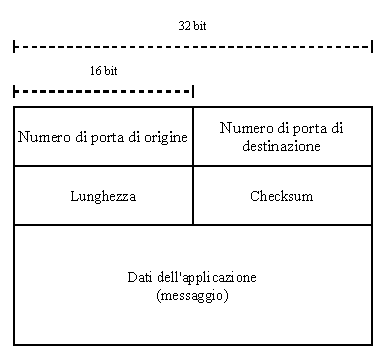
\includegraphics[width=0.7\textwidth]{img/segmento_udp.pdf}
		\caption{Struttura segmento nel protocollo UDP.}
	\end{figure}

	\noindent
	I \textbf{numeri di porta} consentono all’host di destinazione di trasferire i dati applicativi al processo corretto.\newline

	\noindent
	Il \textbf{campo lunghezza} specifica il numero di byte del segmento UDP (intestazione più dati). Un valore esplicito di lunghezza è necessario perché la grandezza del campo dati può essere diversa tra un segmento e quello successivo.\newline
	
	\noindent
	L'host ricevente utilizza il \textbf{checksum} per verificare se sono avvenuti errori nel segmento.
	
	\newpage
	
	\noindent
	\textcolor{Red3}{\textbf{\underline{Protocollo TCP}}}\newline
	
	\noindent
	Nel protocollo TCP il segmento è formato da campi intestazione e di un campo contenente un blocco di dati proveniente dall’applicazione. I campi intestazione formano in totale 20 byte, ovvero 12 in più rispetto a UDP.
	\begin{figure}[!htp]
		\centering
		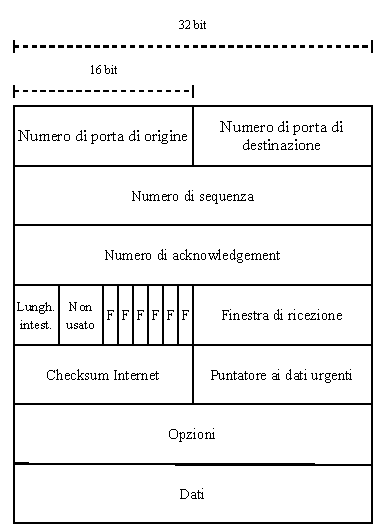
\includegraphics[width=0.8\textwidth]{img/segmento_tcp.pdf}
		\caption{Struttura segmento nel protocollo TCP.}
	\end{figure}

	\noindent
	L'\textbf{intestazione} include:
	\begin{itemize}
		\item \textbf{\underline{Numeri di porta di origine}} e \textbf{\underline{di destinazione}}, utilizzati per il \emph{multiplexing} (processo di costruzione del messaggio) e \emph{demultiplexing} (processo di scomposizione del messaggio).
		
		\item Il campo \textbf{\underline{numero di sequenza}} (\emph{sequence number}) e il campo \textbf{numero di acknowledgement} (\emph{acknowledgment number}), entrambi di 32 bit, vengono utilizzati dal mittente e dal destinatario TCP per implementare il trasferimento dati affidabile.
		
		\item Il campo \textbf{\underline{lunghezza dell'intestazione}} (\emph{header length}), di 4 bit, specifica la lunghezza dell’intestazione TCP in multipli di 32 bit. L’intestazione TCP ha lunghezza variabile a causa del tempo delle opzioni TCP. Generalmente, il campo delle opzioni è vuoto e, pertanto, la lunghezza consueta è di 20 byte.
		
		\item Il campo \textbf{\underline{flag}} (indicato con le lettere F nella figura) è di 6 bit:
		\begin{itemize}
			\item \textbf{ACK} viene usato per indicare che il valore trasportato nel campo di acknowledgement è valido, ovvero il segmento contiene un acknowledgement per un segmento che è stato ricevuto con successo.
			
			\item \textbf{RST, SYN, FIN} vengono utilizzati per impostare e chiudere la connessione.
			
			\item \textbf{CWR, ECE} sono usati nel controllo di congestione esplicito.
			
			\item \textbf{PSH} se ha il valore 1 vuol dire che il destinatario dovrebbe inviare immediatamente i dati al livello superiore.
			
			\item \textbf{URG} indica che il segmento presenta dati che sono stati marcati \dquotes{urgenti} dal livello superiore (solo il mittente ha questa possibilità).
		\end{itemize}
	
		\item Il campo \textbf{\underline{finestra di ricezione}} (\emph{receive window}), di 16 bit, viene utilizzato per il controllo di flusso, ovvero per indicare il numero di byte che il destinatario è disposto ad accettare.
		
		\item Il campo \textbf{\underline{checksum}} di 16 bit è utilizzato per rilevare errori sui bit in un pacchetto trasmesso.
		
		\item Il campo \textbf{\underline{puntatore ai dati urgenti}} è di 16 bit. Quando ci sono dati urgenti, TCP deve informare l’entità destinataria al livello superiore e passarle un puntatore alla fine dei dati urgenti.
		
		\item Il campo \textbf{\underline{opzioni}} (\emph{options}) è facoltativo e di lunghezza variabile. Viene utilizzato quando mittente e destinatario negoziano la dimensione massima del segmento (\emph{Maximum Segment Size}) o come fattore di scala per la finestra nelle reti ad alta velocità.
	\end{itemize}
	\fbox{%
		\parbox{\textwidth}{%
			\textcolor{Red3}{\textbf{\emph{Cos'è MSS?}}}\newline
			La massima quantità di dati prelevabili e posizionabili in un segmento viene limitata dalla \textcolor{Red3}{\textbf{dimensione massima di segmento}} (MSS, \emph{maximum segment size}). Questo valore viene generalmente impostato determinando prima la lunghezza del frame più grande che può essere inviato a livello di collegamento dall’host mittente locale, ovvero la cosiddetta \textcolor{Red3}{\textbf{unità trasmissiva massima}} (MTU, \emph{maximum transmission unit}).
		}%
	}\newline
	
	\noindent
	I \textbf{campi} presenti all’interno del TCP hanno delle porte. I numeri di porta sono di 16 bit e vanno da 0 a 65535, quelli che vanno da 0 a 1023 sono chiamati \textbf{numeri di porta noti} (\emph{well-know port number}) e sono riservati per essere usati da protocolli applicativi ben noti quali HTTP (porta 80) e FTP (porta 21). (l’elenco dei numeri di porta noti è fornito nell’RFC 1700, la sua versione aggiornata si trova al link: \href{http://www.iana.org}{iana.org})
	
	\newpage
	
	\noindent
	Il \textbf{numero di sequenza per un segmento} è il numero nel flusso di byte del primo byte di segmento. Per esempio, supponiamo che un processo nell’Host A voglia inviare un flusso di dati a un processo sull’Host B su una connessione TCP. TCP sull’Host A numera implicitamente ogni byte del flusso di dati. Ipotizziamo che il flusso di dati consista in un file da 500'000 byte, che la MSS valga 1000 byte e che il primo byte del flusso sia numerato con 0. TCP costruisce 500 segmenti per questo flusso di dati ($500'000 \div 1000$). Al primo segmento viene assegnato numero di sequenza 0, al secondo 1000, al terzo 2000 e così via. Ogni numero di sequenza viene inserito nel campo numero di sequenza dell’intestazione del segmento TCP appropriato. Il numero di acknowledgement che l’Host A scrive nei propri segmenti è il numero di sequenza del byte successivo che l’Host A attende dall’Host B. Facciamo alcuni esempi.\newline
	
	\noindent
	Supponiamo che l’Host A abbia ricevuto da B tutti i byte numerati da 0 a 535 e che A stia per mandare un segmento all’Host B. L’Host A è in attesa del byte 536 e dei successivi byte nel flusso di dati di B. pertanto, l’Host A scrive 536 nel campo del numero di acknowledgement del segmento che spedisce a B.\newline
	
	\noindent
	Un ulteriore esempio. Supponiamo che l’Host A abbia ricevuto un segmento dall’Host B contenente i byte da 0 a 535 e un altro segmento contenente i byte da 900 a 1000. Per qualche motivo l’Host A non ha ancora ricevuto i byte da 536 a 899. In questo esempio, l’Host A sta ancora attendendo il byte 536 (e i successivi) per ricreare il flusso di dati di B. perciò il prossimo segmento di A destinato a B conterrà 536 nel campo del numero di acknowledgement. Dato che TCP effettua l’acknowledgement solo dei byte fino al primo byte mancante nel flusso, si dice che tale protocollo offre \textbf{acknowledgement cumulativi} (\emph{cumulative acknowledgement}).
	
	\newpage
	
	\section{Fasi di connessione TCP, RTO e RTT}
	
	\subsection{Fasi di connessione TCP}
	
	In questo capitolo si vedranno tre scenari: l’instaurazione di una connessione TCP, quindi la fase iniziale, la chiusura di una connessione TCP, quindi la fase finale, e la perdita di un pacchetto.\newline
	
	\noindent
	Nella \textcolor{Red3}{\textbf{fase iniziale}} (\textbf{handshake a tre vie}), ovvero nella fase di instaurazione della comunicazione, c’è uno scambio di messaggi:
	\begin{enumerate}
		\item \textbf{\underline{[Segmento SYN]}} TCP lato client invia uno speciale segmento al TCP del server.\newline
		Tale segmento è privo di dati, quindi è in \textbf{assenza} del campo \textbf{Dati}.\newline
		Esso contiene solamente il bit \textbf{SYN} a 1 e un \textbf{numero di sequenza iniziale} (\emph{client initial sequence number}). Quest'ultimo valore viene generato casualmente dal client e posto nel campo \textbf{numero di sequenza} (\emph{sequence number}).\newline
		Infine, viene incapsulato in un datagramma IP e inviato al server.
		
		\item \textbf{\underline{[Segmento SYNACK]}} Una volta che il datagramma IP arriva all’host server (ipotizzando che arrivi), il server estrae il segmento dal datagramma, alloca i buffer e le variabili TCP alla connessione e invia un segmento di connessione approvata al client TCP.\newline
		Il segmento è privo di dati, quindi anch’esso è in \textbf{assenza} del campo \textbf{Dati}.\newline
		Esso contiene il campo \textbf{SYN} a 1, il campo \textbf{ACK} e un \textbf{numero di sequenza iniziale} (\emph{server initial sequence number}).\newline
		\textbf{SYN} indica che il segmento è ancora nella fase iniziale.\newline
		\textbf{Numero di acknowledgement} acquisisce il valore del \emph{client initial sequence number} incrementandolo di 1.\newline
		Nel campo \textbf{numero di sequenza} viene inserito il numero di sequenza iniziale generato casualmente dal server (\emph{server initial sequence number}).
		
		\item \textbf{\underline{[Segmento ACK]}} All’arrivo del segmento SYNACK, anche il client alloca buffer e variabili alla connessione. L’host client invia quindi al server un altro segmento in risposta al segmento di connessione approvata dal server.\newline
		Il segmento questa volta \textbf{può} contenere informazioni che vanno dal client verso il server.\newline
		Esso contiene solamente il campo \textbf{numero di acknowledgement} con valore \emph{server initial sequence number} incrementato di 1.\newline
		Il bit \textbf{SYN} è posto a zero poiché la connessione è stata stabilita.
	\end{enumerate}
	Una volta completati i tre passi, gli host client e server possono scambiarsi segmenti contenenti i dati con bit \textbf{SYN} a zero.
	
	\newpage
	
	\noindent
	Nella \textcolor{Red3}{\textbf{fase finale}}, ovvero nella fase di conclusione e chiusura della connessione, supponendo che il client voglia chiudere la connessione, i messaggi sono:
	\begin{enumerate}
		\item Il processo applicativo client invia un comando di chiusura, che forza il client TCP a inviare un segmento TCP speciale al processo server.\newline
		L’intestazione presenta solo il campo \textbf{FIN} ad 1.
		
		\item Quando il server riceve il segmento di chiusura, risponde inviando un acknowledgement al client. Quindi il server invia un vero e proprio segmento di shutdown.\newline
		Ancora una volta, l'intestazione presenta solamente il campo \textbf{FIN} ad 1.
		
		\item Infine, come accade nella fase iniziale, il client conclude la fase finale inviando un ultimo messaggio di acknowledgement come risposta.
	\end{enumerate}
	Alla fine di questo scambio, tutte le risorse degli host risultano deallocate.
	
	\newpage
	
	\subsection{Caso di perdita: RTO e calcolo RTT}
	
	Prima di parlare del caso in cui un pacchetto viene perso nella connessione di tipo TCP, è doveroso introdurre l’indice RTO e RTT.\newline
	
	\noindent
	L’\textcolor{Red3}{\textbf{indice RTT}} (\emph{Round Trip Time}) è la quantità di tempo che intercorre tra l’istante di invio del segmento (ossia quando viene passato a IP) e quello di ricezione dell’acknowledgement del segmento.\newline
	
	\noindent
	Invece di misurare per ogni segmento il suo RTT, il protocollo TCP valuta il \emph{round trip time} solo per uno dei segmenti trasmessi e per cui non si è ancora ricevuto acknowledgement. Questo comporta la misurazione di un nuovo valore a ogni RTT, circa.\newline
	
	\noindent
	Ovviamente, tali valori variano a seconda del segmento, a seconda della congestione nei router e a seconda del carico sui sistemi periferici. A causa di questa fluttuazione, ogni valore RTT può essere atipico. Per effettuare una stima naturale, si calcola una media di valori del RTT, ovvero \emph{\textbf{Estimated}} RTT. Tale valore è una media ponderata dei valori del RTT ed attribuisce maggiore importanza ai valori recenti rispetto a quelli vecchi. Tuttavia, è del tutto normale questa valutazione poiché i primi riflettono meglio la congestione attuale della rete.\newline
	
	\label{RTO}\noindent
	L'\textcolor{Red3}{\textbf{indice RTO}} (\emph{Retrasmission Time-Out}) è il tempo di ritrasmissione di un pacchetto. All’invio di un pacchetto, parte un timer che indica il range di tempo in cui il server deve rispondere. Nel caso in cui il server non riesca a rispondere entro questo intervallo, viene inviato nuovamente lo stesso pacchetto al server.\newline
	
	\noindent
	Questo indice viene impostato prendendo il \emph{Estimated} RTT e aggiungendo un certo margine che dovrebbe essere grande quando c’è molta fluttuazione dei valori RTT e piccolo in caso contrario. Inizialmente il valore è pari a 1 secondo.\newline
	
	\noindent
	\textbf{In caso di perdita}, TCP \textbf{ritrasmette il segmento con il più basso numero di sequenza che non abbia ancora ricevuto acknowledgement}. Tuttavia, ogni volta che questo si verifica, TCP imposta il successivo RTO al doppio del valore precedente. In caso di perdite continue, RTO continua a raddoppiare.\newline
	
	\noindent
	Uno dei casi in cui RTO aumenta è dovuto al fatto che la rete potrebbe essere congestionata, ovvero troppi pacchetti arrivano presso una (o più) code dei router nel percorso tra l’origine e la destinazione, provocando l’eliminazione dei pacchetti e/o lunghi ritardi di accodamento.
	
	\newpage
	
	\subsection{\textcolor{Red3}{Esame - Blocco CIDR, subnetting e broadcast}}
	
	\begin{center}
		\large
		\textcolor{Green4}{\textbf{Tema d'esame - 05/07/2013, esercizio 2}}
	\end{center}
	
	\noindent
	Si determini il blocco CIDR più piccolo della rete sapendo che si devono creare 3 reti LAN con i seguenti vincoli:
	\begin{itemize}
		\item LAN1 con 300 host
		\item LAN2 con 40 host
		\item LAN3 con 90 host
	\end{itemize}
	Sapendo che l'indirizzo di broadcast della LAN3 è: $148.12.79.255$.\newline
	
	\noindent
	\textbf{Prima di tutto}, si ricorda che l’indirizzo broadcast è un indirizzo in cui il suffisso, nella forma binaria, è formato da soli bit posti a 1.\newline
	
	\noindent
	Il \textbf{primo passo} degli esercizi con il blocco CIDR e il \emph{subnetting} è stabilire il numero di bit da assegnare a ciascuna rete seguendo i vincoli imposti:
	\begin{itemize}
		\item LAN1 necessita di 300 host e l'unica potenza del 2 che copre tale numero è $2^{9} = 512$;
		\item LAN2 necessita di 40 host e l'unica potenza del 2 che copre tale numero è $2^{6} = 64$;
		\item LAN3 necessita di 90 host e l'unica potenza del 2 che copre tale numero è $2^{7} = 128$.
	\end{itemize}
	La somma dei risultati delle potenze, ovvero il numero di indirizzi che dovrà almeno avere questa rete è:
	\begin{equation*}
		512 + 64 + 128 = 704
	\end{equation*}
	L'unica potenza del 2 che riesce a coprire tale valore è $2^{10}$. Per cui servono 10 bit di suffisso per ricoprire almeno 704 host.\newline
	
	\noindent
	Grazie a questo dato si può ricavare il prefisso di rete: $2^{32} \div 2^{10}=2^{22}$. A questo punto ci sono tutti i dati per costruire l’indirizzo di rete partendo dall’unico indirizzo derivato da esso, ovvero l’indirizzo di broadcast.\newline
	
	\noindent
	Si effettua la traduzione dell’indirizzo di broadcast ($148.12.79.255$) in binario:
	\begin{equation*}
		\binaryaddresspointed{10010100}{00001100}{01001111}{11111111}
	\end{equation*}
	Sapendo che i primi 22 bit sono di prefisso, poniamo i restanti bit di suffisso a zero e otteniamo il blocco di rete CIDR più piccolo:
	\begin{equation*}
		\binaryaddresspointed{10010100}{00001100}{01001100}{00000000}
	\end{equation*}
	Convertendo nuovamente l’indirizzo in notazione decimale puntata, il \textbf{blocco CIDR più piccolo} è: $148.12.76.0/22$.\newline
	
	\noindent
	Per trovare le 3 LAN si procede con la creazione di sottoreti partendo dall’indirizzo di rete appena trovato e aumentando il prefisso:
	\begin{gather*}
		\binaryaddresspointed{10010100}{00001100}{010011\textcolor{Red3}{\boldsymbol{0}}0}{00000000}/23 \\
		\binaryaddresspointed{10010100}{00001100}{010011\textcolor{Red3}{\boldsymbol{1}}0}{00000000}/23
	\end{gather*}
	Il primo indirizzo trovato si può subito assegnare alla LAN1 che richiedeva almeno 300 host e con un indirizzo del genere ne vengono messi a disposizione massimo ($2^{9}$) 512. Quindi, l’indirizzo della \textbf{LAN1 in notazione decimale puntata}: $148.12.76.0/23$.\newline
	
	\noindent
	Con il secondo indirizzo si costruiscono nuovamente altre due sottoreti per cercare di rispettare i vincoli imposti:
	\begin{gather*}
		\binaryaddresspointed{10010100}{00001100}{0100111\textcolor{Red3}{\boldsymbol{0}}}{00000000}/24 \\
		\binaryaddresspointed{10010100}{00001100}{0100111\textcolor{Red3}{\boldsymbol{1}}}{00000000}/24
	\end{gather*}
	Gli indirizzi trovati non soddisfano nessun vincolo. Precisamente entrambi potrebbero contenere sia la LAN numero 2 e 3, ma non sarebbero ottimizzate perché con il suffisso di 7 bit si avrebbero 128 indirizzi contro gli 8 bit con 256 indirizzi.\newline
	
	\noindent
	Per cui, si utilizza il primo indirizzo per suddividere ancora la rete e il secondo indirizzo si lascia libero per operazioni future. Quindi, un’altra suddivisione utilizzando solamente il primo indirizzo porterebbe a:
	\begin{gather*}
		\binaryaddresspointed{10010100}{00001100}{01001110}{\textcolor{Red3}{\boldsymbol{0}}0000000}/25 \\
		\binaryaddresspointed{10010100}{00001100}{01001110}{\textcolor{Red3}{\boldsymbol{1}}0000000}/25
	\end{gather*}
	Il primo indirizzo soddisfa il vincolo imposto dalla terza LAN, per cui scrivendo l’indirizzo della \textbf{LAN3 in notazione decimale puntata}: $148.12.78.0/25$.\newline
	
	\noindent
	Per l’ultima LAN serve creare un’altra sottorete partendo dal secondo indirizzo, quindi:
	\begin{gather*}
		\binaryaddresspointed{10010100}{00001100}{01001110}{1\textcolor{Red3}{\boldsymbol{0}}000000}/26 \\
		\binaryaddresspointed{10010100}{00001100}{01001110}{1\textcolor{Red3}{\boldsymbol{1}}000000}/26
	\end{gather*}
	Il primo indirizzo rispetta i vincoli imposti dalla seconda LAN, per cui scrivendo l’indirizzo della \textbf{LAN2 in notazione decimale puntata}: $148.12.78.128/26$.\newline
	Infine, il secondo indirizzo rimane libero per il futuro.
	
	\newpage
	
	\section{Controllo di flusso (TCP), finestra e ripetizione selettiva}
	
	\subsection{Controllo di flusso (TCP)}
	
	In una comunicazione con connessione di tipo TCP, gli host posseggono un buffer (registro temporaneo, chiamato anche \emph{buffer di ricezione}) in cui vengono salvati i \emph{byte} corretti e in sequenza. Ovviamente tale registro ha una capienza limitata e l’applicazione mittente potrebbe mandare in overflow il buffer di ricezione del destinatario inviando molti dati troppo rapidamente.\newline
	
	\noindent
	\underline{Per risolvere l’overflow del buffer di ricezione}, il protocollo TCP offre un \textcolor{Red3}{\textbf{servizio di controllo di flusso}} (\emph{flow-control service}). Esso è un servizio di confronto sulla velocità poiché paragona la frequenza di invio del mittente con quella di lettura dell’applicazione ricevente.\newline
	
	\noindent
	\fbox{%
		\parbox{\textwidth}{%
			\begin{center}
				\textcolor{Red3}{\textbf{\emph{Attenzione!} Flusso vs Congestione}}
			\end{center}
			Esiste una sostanziale \textbf{differenza} tra il \textbf{controllo di flusso} e il \textbf{controllo di congestione}.\newline
			Nel \textbf{controllo di flusso}, il protocollo evita che il buffer di ricezione del destinatario vada in overflow.\newline
			Nel \textbf{controllo di congestione} (\emph{congestion control}), il protocollo evita che ci siano carichi troppi elevati e code troppo consistenti sui buffer, causa principale di rallentamenti nella rete.
		}%
	}\newline
	\:\newline
	
	\noindent
	TCP garantisce il controllo di flusso grazie all’obbligo di mantenimento di una variabile chiamata \textcolor{Red3}{\textbf{finestra di ricezione}} (\emph{receive window}) gestita dal mittente. Essa fornisce al mittente un’indicazione dello spazio libero disponibile nel buffer del destinatario. Per approfondire l’argomento e vedere la sua applicazione, nella prossima pagina verrà effettuato un esempio di trasferimento di file.
	\newpage
	
	\begin{center}
		\large
		\textcolor{Green4}{\textbf{\emph{Esempio}}}
	\end{center}

	\noindent
	Supponiamo che l’\textsf{Host A} stia inviando un file di grandi dimensioni all’\textsf{Host B} su una connessione di tipo TCP, quindi affidabile e con controllo di flusso.\newline
	
	\noindent
	TCP obbliga l’\textsf{Host B} ad allocare un \textbf{buffer di ricezione} per la connessione, la dimensione di tale buffer sarà denotata con \textbf{\textsf{RcvBuffer}} (\emph{Receive Buffer}) ed ogni tanto il processo applicativo dell’\textsf{Host B} legge dal buffer.\newline
	
	\noindent
	Si definiscono le seguenti variabili:
	\begin{itemize}
		\item \textbf{\textsf{LastByteRead}}: numero dell'\textbf{ultimo byte}, nel flusso di dati, che il processo applicativo in B ha \textbf{letto dal buffer}.

		\item \textbf{\textsf{LastByteRcvd}}: numero dell'\textbf{ultimo byte}, nel flusso di dati, che proviene dalla rete e che è stato \textbf{copiato nel buffer di ricezione} di B.
	\end{itemize}
	Dato che il protocollo TCP \textbf{evita} che il buffer allocato vada in overflow, si può affermare con certezza la seguente disuguaglianza:
	\begin{equation*}
		LastByteRcvd - LastByteRead \le RcvBuffer
	\end{equation*}
	La \textbf{finestra di ricezione}, indicata con \textbf{\textsf{rwnd}}, viene impostata alla quantità di spazio disponibile nel buffer, ovvero:
	\begin{equation*}
		rwnd = RcvBuffer - \left[LastByteRcvd - LastByteRead\right]
	\end{equation*}
	Dato che lo spazio disponibile varia col tempo, \textsf{rwnd} è dinamica.\newline
	
	\noindent
	Adesso che sono state definite le basi, come viene usata la variabile rwnd per offrire il servizio di controllo di flusso?\newline
	
	\noindent
	L’\textsf{Host B} comunica all’\textsf{Host A} quanto spazio disponibile è presente nel buffer della connessione, scrivendo il valore corrente di \textsf{rwnd} nel campo apposito dei segmenti che manda ad A. L’\textsf{Host B} inizializza \textsf{rwnd} con il valore \textsf{RcvBuffer} e, ovviamente, deve tenere traccia di variabili specifiche per ogni connessione.\newline
	
	\noindent
	A sua volta, l’\textsf{Host A} tiene traccia di due variabili, \textbf{\textsf{LastByteSent}} e \textbf{\textsf{LastByteAcked}}, il cui significato è rispettivamente \dquotes{\textbf{ultimo byte mandato}} e \dquotes{\textbf{ultimo byte per cui si è ricevuto acknowledgement}}.\newline
	
	\noindent
	Si noti che la differenza tra i valori di queste due variabili esprime la \textbf{quantità di dati spediti da A per cui non si è ancora ricevuto un acknowledgement}. Mantenendo la quantità di dati senza acknowledgement sotto il valore di \textsf{rwnd}, si garantisce che l’\textsf{Host A} non mandi in overflow il buffer di ricezione dell’\textsf{Host B}. Quindi, l’\textsf{Host A} si assicura che per tutta la durata della connessione sia rispettata la disuguaglianza:
	\begin{equation*}
		LastByteSent - LastByteAcked \le rwnd
	\end{equation*}\newpage

	\noindent
	Tuttavia, questo esempio presenta un problema. Si supponga che l’\textsf{Host B} si riempia, quindi con \textsf{rwnd} uguale a zero, notifichi l’\textsf{Host A} e, infine, non abbia più nulla da inviare ad A. Quello che succede è che TCP non invia nuovi segmenti con nuovi valori di \textsf{rwnd} poiché l’\textsf{Host B} non ha più dati da inviare o acknowledgement da mandare. Questo comporta che l’\textsf{Host A} non venga notificato nel momento in cui l’\textsf{Host B} svuoti il buffer. Quindi, si crea un’inabilitazione dell’\textsf{Host A}!\newline
	
	\noindent
	Per \textbf{risolvere tale problema} basta che l’\textsf{Host A} continui a inviare periodicamente segmenti con un byte di dati quando la finestra di ricezione di B è zero. Il destinatario, ovvero l’\textsf{Host B}, risponderà a questi segmenti con un acknowledgement. Prima o poi il buffer inizierà a svuotarsi e i riscontri conteranno un valore non nullo per \textsf{rwnd}.\newline
	
	\noindent
	In sintesi, c’è un continuo scambi di messaggi per controllare che la finestra sia sempre uguale a zero.
	
	\subsection{Ripetizione selettiva}
	
	I \textcolor{Red3}{\textbf{protocolli a ripetizione selettiva}} (SR, \emph{selection-repeat protocol}) \emph{evitano} le ritrasmissioni non necessarie facendo ritrasmettere al mittente solo quei pacchetti su cui esistono sospetti di errore, ovvero smarrimento o alterazione.\newline
	
	\noindent
	Questo protocollo \textbf{obbliga} il destinatario ad inviare acknowledgement specifici per i pacchetti ricevuti in modo corretto.\newline
	
	\noindent
	\textbf{Per esempio}, se un segmento non ricevesse l’acknowledgement relativo dal destinatario, allo scadere del RTO (\emph{Retrasmission Time-Out}) entrerebbe in gioco il protocollo di ripetizione selettiva, il quale invierebbe al destinatario solamente quel pacchetto che non ha ricevuto il suo acknowledgement.\newpage
	
	\section{Algoritmo di controllo di congestione di TCP}
	
	Generalmente TCP capisce quando aumentare e diminuire la velocità di trasmissione dei dati da parte del mittente grazie ad alcune linee guida:
	\begin{itemize}
		\item Un segmento perso implica congestione, quindi i tassi di trasmissione del mittente TCP dovrebbero essere decrementati quando un segmento viene perso.
		\item Un acknowledgement indica che la rete sta consegnando i segmenti del mittente al ricevente e quindi il tasso di trasmissione del mittente può essere aumentato quando arriva un acknowledgement non duplicato.
		\item Rilevamento della larghezza di banda tramite alcune tecniche.
	\end{itemize}
	Nonostante tali linee guida, esiste un \textcolor{Red3}{\textbf{algoritmo di congestione di TCP}} per controllare la congestione. Esso presenta tre componenti o fasi principali: \textbf{\emph{slow start}}, \textbf{\emph{congestion avoidance}} e \textbf{\emph{fast recovery}}. I primi due componenti sono obbligatori di TCP e differiscono nel modo in cui aumentano la grandezza di \textsf{cwnd}\footnote{\emph{congestion window}, finestra di congestione, ovvero la finestra di dati trasmessi e non ancora riscontrati dal mittente poiché risposta acknowledgement mancante} in risposta agli acknowledgement ricevuti.  Al contrario, la \emph{fast recovery} è suggerita, ma non obbligatoria, per i mittenti TCP.\newpage
	
	\subsection{Slow start}
	Quando si stabilisce una connessione TCP, il valore di \textsf{cwnd} viene in genere inizializzato a 1 MSS (\emph{Maximum Segment Size}). Questo comporta una velocità di invio iniziale di circa MSS/RTT.\newline
	
	\noindent
	Per esempio, se $MSS = 500$ Byte e $RTT = 200$ ms, la velocità iniziale è solo di circa $20$ kbps. Tuttavia, la banda disponibile inizialmente potrebbe essere molto più grande. Per questo motivo, durante la fase iniziale, il valore della \textbf{\emph{congestion window}} (\textsf{cwnd}) \textbf{parte da 1 MSS e si incrementa di 1 MSS ogni volta che un segmento trasmesso riceve un acknowledgement} (detta \textcolor{Red3}{\textbf{\emph{slow start}}} per l’inizio adagio).\newline
	
	\noindent
	\textbf{Per esempio}, nel momento di scambio di dati tra due host dopo l'handshaking, accade che:
	\begin{enumerate}
		\item Il mittente invia il \textbf{primo segmento} nella rete e attende un riscontro:
		\begin{enumerate}[label=\alph*.]
			\item Se il mittente riceve un acknowledgement del segmento, quindi \textbf{senza} avere nessuna \textbf{perdita}, esso incrementa la finestra di congestione di 1 MSS.\newline
			Adesso il mittente ne potrà inviare due di segmenti poiché la sua \textsf{cwnd} sarà di 2 MSS.\newline
			Assumendo che vengano inviati i due segmenti e si ricevano i due acknowledgement rispettivi, il destinatario, come risposta, comunica la grandezza della \textsf{cwnd} a 4 poiché per ogni segmento ricevuto correttamente ha incrementato la finestra di 1.\newline
			E così via.
			
			\item Se il mittente non riceve un acknowledgement del segmento appena inviato, si manifesta un evento di \textbf{perdita} (e quindi di congestione).\newline
			In questo caso, il mittente pone il valore della \textsf{cwnd} pari a 1 e inizia nuovamente il processo di \emph{slow start} (punto a).\newline
			Oltre ad iniziare da capo, \textbf{modifica il valore della variabile \textsf{ssthresh}} (\emph{slow start threshold}, in italiano \dquotes{soglia di \emph{slow start}}) a $\textbf{cwnd} \div 2$: ovvero metà del valore che aveva la finestra di congestione quando è stata rilevata una perdita, o meglio una congestione.
		\end{enumerate}
	\end{enumerate}
	La conseguenza dell’evento \dquotes{1.\emph{a}}, cioè senza perdita, ha come effetto il raddoppio della velocità trasmissiva a ogni RTT. È possibile affermare che nel protocollo TCP, la \textbf{velocità di trasmissione parte lentamente, ma cresce in modo esponenziale} durante la fase di \emph{slow start}.\newline
	
	\noindent
	La fase di \emph{slow start} può \textbf{terminare} con una perdita: come spiegato al punto \emph{b}, oppure quando il valore della \textsf{cwnd} raggiunge o supera il valore della \textsf{ssthresh}. Il motivo è dovuto al fatto che \textsf{ssthresh} è il limite e il suo superamento aumenta le probabilità di congestione, ovvero di perdita.\newline
	
	\noindent
	Una volta terminata la \emph{slow start}, TCP entra nella fase di \textbf{\emph{congestion avoidance}}.\newpage
	
	\subsection{Congestion avoidance}
	
	Quando TCP entra nello stato di \textcolor{Red3}{\textbf{\emph{congestion avoidance}}} adotta un approccio più conservativo. Invece di raddoppiare il valore di \textsf{cwnd} ogni RTT come nello \emph{slow start}, l’aumento della \textsf{cwnd} avviene di 1 MSS ogni RTT.\newline
	
	\noindent
	L'\textbf{aumento} può avvenire tramite il seguente metodo (più comune).\newline
	Il mittente incrementa la propria \textbf{cwnd} di $MSS \times \left(\frac{MSS}{\textsf{cwnd}}\right)$ byte ogni qualvolta riceva un nuovo acknowledgement.\newline
	\textcolor{Green4}{\textbf{Per esempio}}, supponendo che MSS vale $1'460$ byte e \textsf{cwnd} $14'600$ byte, allora in un RTT vengono spediti dieci segmenti. Questo calcolo è possibile eseguirlo mentalmente poiché se i dati da trasmettere devono essere $14'600$, ma ogni segmento può avere al massimo una grandezza di $1'460$, allora considerando un segmento come $1'460$ byte, si dovranno inviare 10 segmenti per avere il pacchetto completo.\newline
	In questo esempio, la \textsf{cwnd} aumenterà di $1/10$ della MSS ogni qualvolta riceverà 1 acknowledgement di un segmento inviato. Quindi una volta ricevuti tutti i 10 acknowledgement dei 10 segmenti inviati, la \textsf{cwnd} sarà aumentata di 1 MSS, ovvero di $1460$ byte.\newline
	
	\noindent
	Al contrario, la fase di incremento si \textbf{interrompe} quando si esaurisce il tempo del RTO (\emph{Retrasmission Time-Out}). Il comportamento successivo all’interruzione è identico a quello dello \emph{slow start}:
	\begin{itemize}
		\item Il valore di \textsf{\textbf{cwnd}} è posto uguale a 1 MSS;
		\item Il valore di \textsf{\textbf{ssthresh}} viene impostato alla metà del valore di \textsf{cwnd} al momento del time-out.
	\end{itemize}
	Infine, TCP entra nella fase di \emph{fast recovery}.
	
	\subsection{Fast recovery}
	
	Una volta terminato il periodo di attesa del RTO si passa dallo stato di \textcolor{Red3}{\textbf{\emph{fast recovery}}} a quello di \emph{slow start} dopo avere effettuato le stesse azioni presenti sia in \emph{slow start} che in \emph{congestion avoidance}. Queste azioni sono: il valore di \textsf{cwnd} posto a 1 MSS e il valore di \textsf{ssthresh} è impostato a metà del valore di \textsf{cwnd} nel momento in cui si è riscontrato l’evento di perdita.\newline
	
	\noindent
	\textbf{Attenzione!} Questo metodo \textbf{non} è obbligatorio, viene solo raccomandato. Una prima versione di TCP, nota come \textbf{TCP Tahoe}, portava la finestra di congestione a 1 MSS ed entrava nella fase di \emph{slow start} dopo qualsiasi tipo di evento di perdita. La versione più recente, \textbf{TCP Reno}, adotta invece \emph{fast recovery}.\newpage
	
	\section{Dettaglio dell'algoritmo di controllo di congestione di TCP}
	
	\subsection{Algoritmo}
	
	Nello scorso capitolo è stato introdotto l'algoritmo di controllo di congestione del protocollo TCP. Al contrario, in questo capitolo l'algoritmo verrà approfondito e utilizzato per svolgere esercizi.\newline
	
	\noindent
	Prima di iniziare la descrizione dell'algoritmo, è necessario tenere in \textbf{considerazione quattro variabili}:
	\begin{itemize}
		\item \textbf{\textsf{CWND}} (\emph{Congestion Window}), ovvero la dimensione della finestra della trasmissione.
		
		\item \textbf{\textsf{RTO}} (\emph{Retrasmission Time-Out}), calcolato dinamicamente, è il tempo che intercorre dall'invio del segmento al momento in cui il protocollo realizza che c'è un evento di congestione (paragrafo~\ref{RTO}).
		
		\item \textbf{\textsf{RCV WND}} (\emph{Receive Window}), ovvero la dimensione massima della finestra di ricezione.
		
		\item \textbf{\textsf{SSTHRESH}} (\emph{Slow Start Threshold}), ovvero la soglia per capire se utilizzare l'algoritmo \emph{slow start} o passare all'algoritmo \emph{congestione avoidance}.
	\end{itemize}
	E nella fase di \textbf{inizializzazione}:
	\begin{itemize}[label=-]
		\item $\textsf{CWND} = 1$;

		\item $\textsf{RCV WND} = $ comunicato dalla destinazione la quale inserisce il valore di tale finestra nel header TCP, precisamente il campo \emph{window};
		
		\item $\textsf{SSTHRESH} = RCV\:WND$ oppure $RCV\:WND \div 2$.
	\end{itemize}
	\newpage\noindent
	Ora che sono state effettuate delle doverose spiegazioni delle variabili necessarie e sono state inizializzate, è possibile \textcolor{Red3}{\textbf{descrivere l'algoritmo di controllo della congestione}}:
	\begin{enumerate}
		\item \textbf{Effettuare la numerazione dei segmenti} finché non si raggiunge la dimensione delle \textsf{CWND} (\emph{congestion window}) ed \textbf{inviare i segmenti} al destinatario;
		
		\item \textbf{Quando arrivano tutti i riscontri} relativi ai segmenti inviati al punto precedente, si controlla \textbf{se il valore della \textsf{CWND} è minore} al valore del limite, ovvero \textbf{della \textsf{SSTHRESH}}:
		\begin{enumerate}
			\item Se \textsf{CWND} è minore della \textsf{SSTHRESH} allora si avvia la fase di \emph{slow start} e la \textsf{CWND} diventa uguale al valore \textbf{minimo} tra:
			\begin{enumerate}
				\item $\textsf{CWND}_{old} + \text{numero di ACK ricevuti}$
				\item \textsf{SSTHRESH}
				\item \textsf{RCV WND}
			\end{enumerate}
			
			\item Se \textsf{CWND} è maggiore della \textsf{SSTHRESH} allora si avvia la fase di \emph{congestion avoidance} e il valore della \textsf{CWND} diventa uguale al valore \textbf{minimo} tra:
			\begin{enumerate}
				\item $\textsf{CWND}_{old} + \frac{\text{numero di ACK ricevuti}}{\textsf{CWND}_{old}}$
				\item \textsf{RCV WND}
			\end{enumerate}
		\end{enumerate}
		
		\item Al contrario, in caso di \textbf{mancanza di un riscontro} di un segmento inviato al punto uno:
		\begin{enumerate}
			\item Si aspetta la fine del tempo di \emph{time-out} scandito dal RTO;
			
			\item Una volta finito il tempo della RTO, la SSTHRESH acquisisce il valore della CWND diviso 2 al momento esatto della perdita;
			
			\item Il nuovo valore della CWND assumerà un valore diverso a seconda dell'algoritmo applicato:
			\begin{enumerate}
				\item Con la versione \textbf{TCP Tahoe}, ovvero la meno recente e quella utilizzata durante il corso, il nuovo valore sarà:
				\begin{equation*}
					\textsf{CWND} = 1
				\end{equation*}
				
				\item Con la versione \textbf{TCP Reno}, ovvero la più recente che utilizza la \emph{fast recovery}:
				\begin{equation*}
					\textsf{CWND} = \textsf{SSTHRESH}
				\end{equation*}
			\end{enumerate}
			
			\item Una volta cambiati i valori necessari, i segmenti vengono ritrasmessi e il nuovo valore RTO diventa il valore precedente moltiplicato per due:
			\begin{equation*}
				\textsf{RTO}_{new} = \textsf{RTO} \times 2
			\end{equation*}
			
			\item Infine, si torna al punto \emph{a}.
		\end{enumerate}
	\end{enumerate}
	\newpage
	
	\subsection{Sintesi algoritmo}
	
	Data l'eventuale difficoltà nel leggere lo schema, si lascia qui di seguito un diagramma di flusso:
	\begin{figure}[!htp]
		\centering
		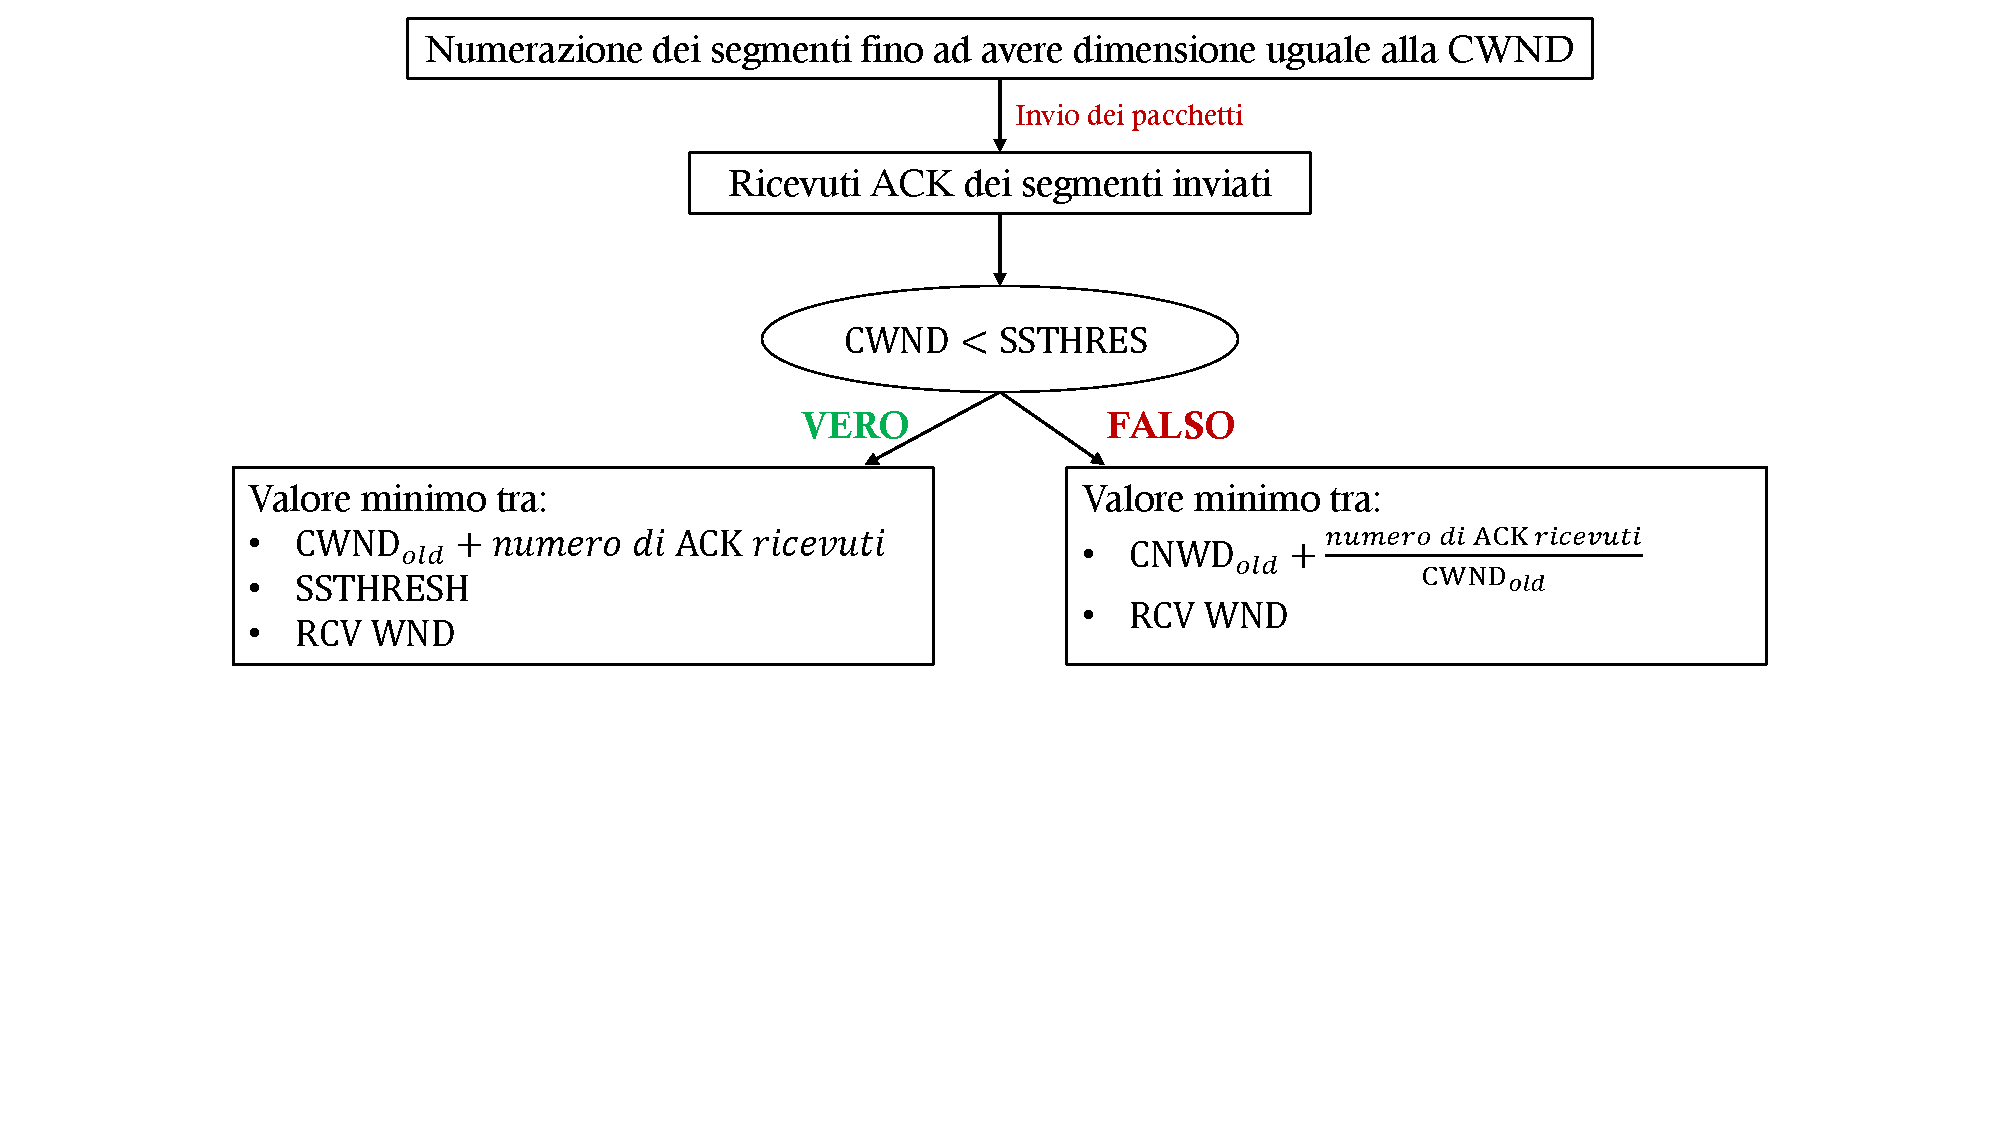
\includegraphics[width=\textwidth]{img/algoritmo_congestione_TCP.pdf}
		\caption{Algoritmo di congestione del protocollo TCP.}
	\end{figure}
	
	\noindent	
	E uno aggiuntivo che si riferisce alle scelte da applicare nel momento in cui vengano persi dei segmenti:
	\begin{figure}[!htp]
		\centering
		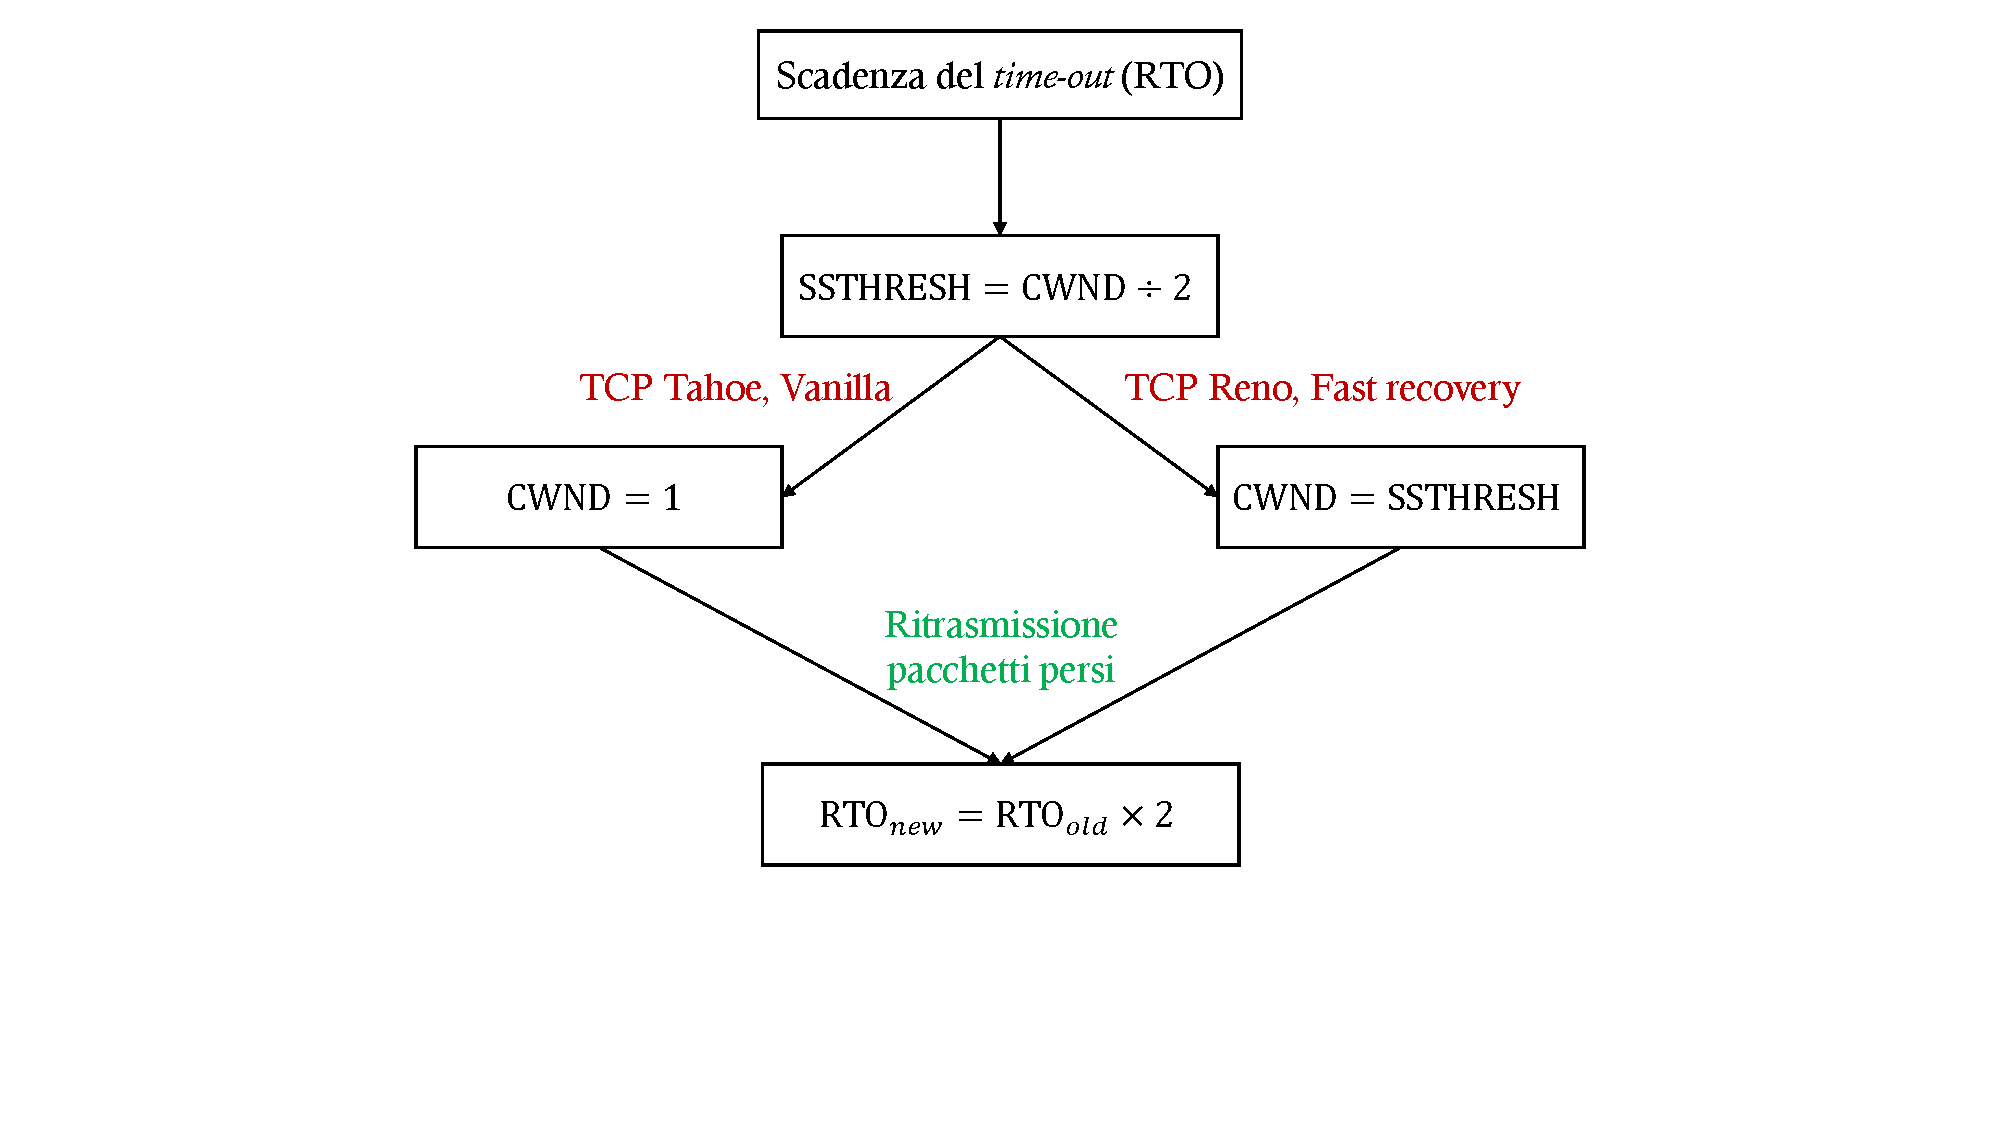
\includegraphics[width=\textwidth]{img/algoritmo_congestione_TCP_perdita.pdf}
		\caption{Algoritmo di congestione del protocollo TCP in \textbf{caso di perdita}.}
	\end{figure}
	\newpage
	
	\subsection{Esempio di congestione}
	
	In questo esempio, si simula l’invio di una serie di pacchetti per studiare lo \emph{slow start} e la \emph{congestion avoidance}. Il mittente A invia dei segmenti al destinatario B; il protocollo TCP inizia con l’algoritmo \emph{slow start}. La \textsf{RCV WND} viene posta e rimane a 16 durante tutto l’esempio, mentre la \textsf{SSTHRESH} parte con il valore 8.
	
	\begin{wrapfigure}{R}{0.5\textwidth}
		\centering
		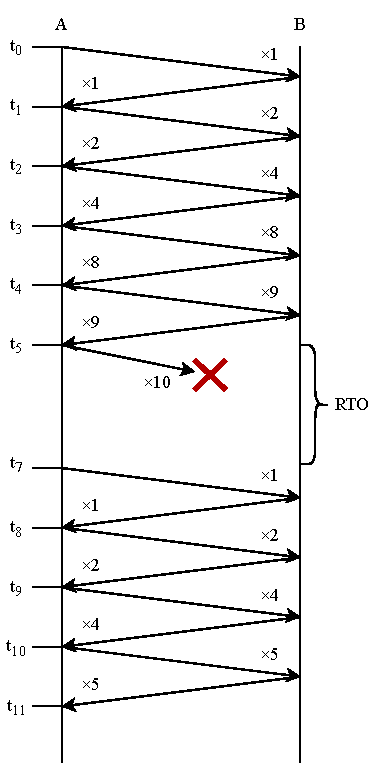
\includegraphics[width=0.5\textwidth]{img/esempio_congestione.pdf}
	\end{wrapfigure}

	\noindent
	Al tempo $t_{0}$ viene inviato il primo segmento dato che la \textsf{CWND} è posta a 1.\newline
	
	\noindent
	All’arrivo del primo \textsf{ACK}, tempo $t_{1}$, l’algoritmo confronta i valori della \textsf{CWND} e della \textsf{SSTHRESH}: la prima è minore della seconda poiché $1 < 8$; per cui si confrontano i tre valori scegliendo il minore. Tra 2 ($\textsf{CWND} + \text{\#ack ricevuti}$), 8 (\textsf{SSTHRESH}) e 16 (\textsf{RCV WND}), il valore più piccolo è 2. Quest’ultimo valore diventerà il nuovo valore della \emph{congestion window}: $\textsf{CWND}_{new} = 2$.\newline
	
	\noindent
	Al tempo $t_{2}$, vengono inviati due segmenti e il processo spiegato precedentemente si ripete.\newline
	
	\noindent
	Il cambiamento degno di nota è al tempo $t_{4}$ quando la \textsf{CWND} passa dal valore 8 al valore 9. Questo accade poiché al tempo $t_{4}$ la \textsf{CWND} è uguale alla \textsf{SSTHRESH} e, seguendo l’algoritmo, si dovrà quindi scegliere il valore minimo tra: 9 ($\frac{\textsf{CWND}_{old} + \left(\text{\#ack ricevuti}\right)}{\textsf{CWND}_{old}}$) e 16 (\textsf{RCV WND}). Il valore minimo è 9, la $\textsf{CWND}_{new}$ diventa 9 e vengono trasmessi i segmenti.\newline
	
	\noindent
	Un’altra osservazione doverosa è quello che succede al tempo $t_{5}$. Il TCP rileva una perdita poiché alla fine del \textsf{RTO} non sono stati ancora ricevuti gli \textsf{ACK}. In quel momento entra in gioco la fase di \dquotes{mancanza di riscontro}, ovvero: il valore della \textsf{SSTHRES} diventa il valore della \textsf{CWND}, al momento della perdita, diviso 2; la $\textsf{CWND}_{new}$ diventa pari a 1 (uso del TCP Tahoe o Vanilla); \textsf{RTO} dei pacchetti ritrasmessi diventa $\textsf{RTO} \times 2$.\newline
	
	\noindent
	Infine, al tempo $t_{7}$ si inizia nuovamente con lo \emph{slow start}.\newpage
	
	\noindent
	Qui di seguito si lascia lo schema utilizzato anche per la risoluzione degli esercizi di questo tipo. Esso presenta sull’asse delle ordinate ($y$) il valore della \textsf{CWND}, mentre sull’asse delle ascisse ($x$) il tempo. Con la linea blu viene rappresentato lo \textsf{SSTHRESH}, mentre con il rosso la \textsf{RCV WND} costante per tutto l’esempio.
	\begin{figure}[!htp]
		\centering
		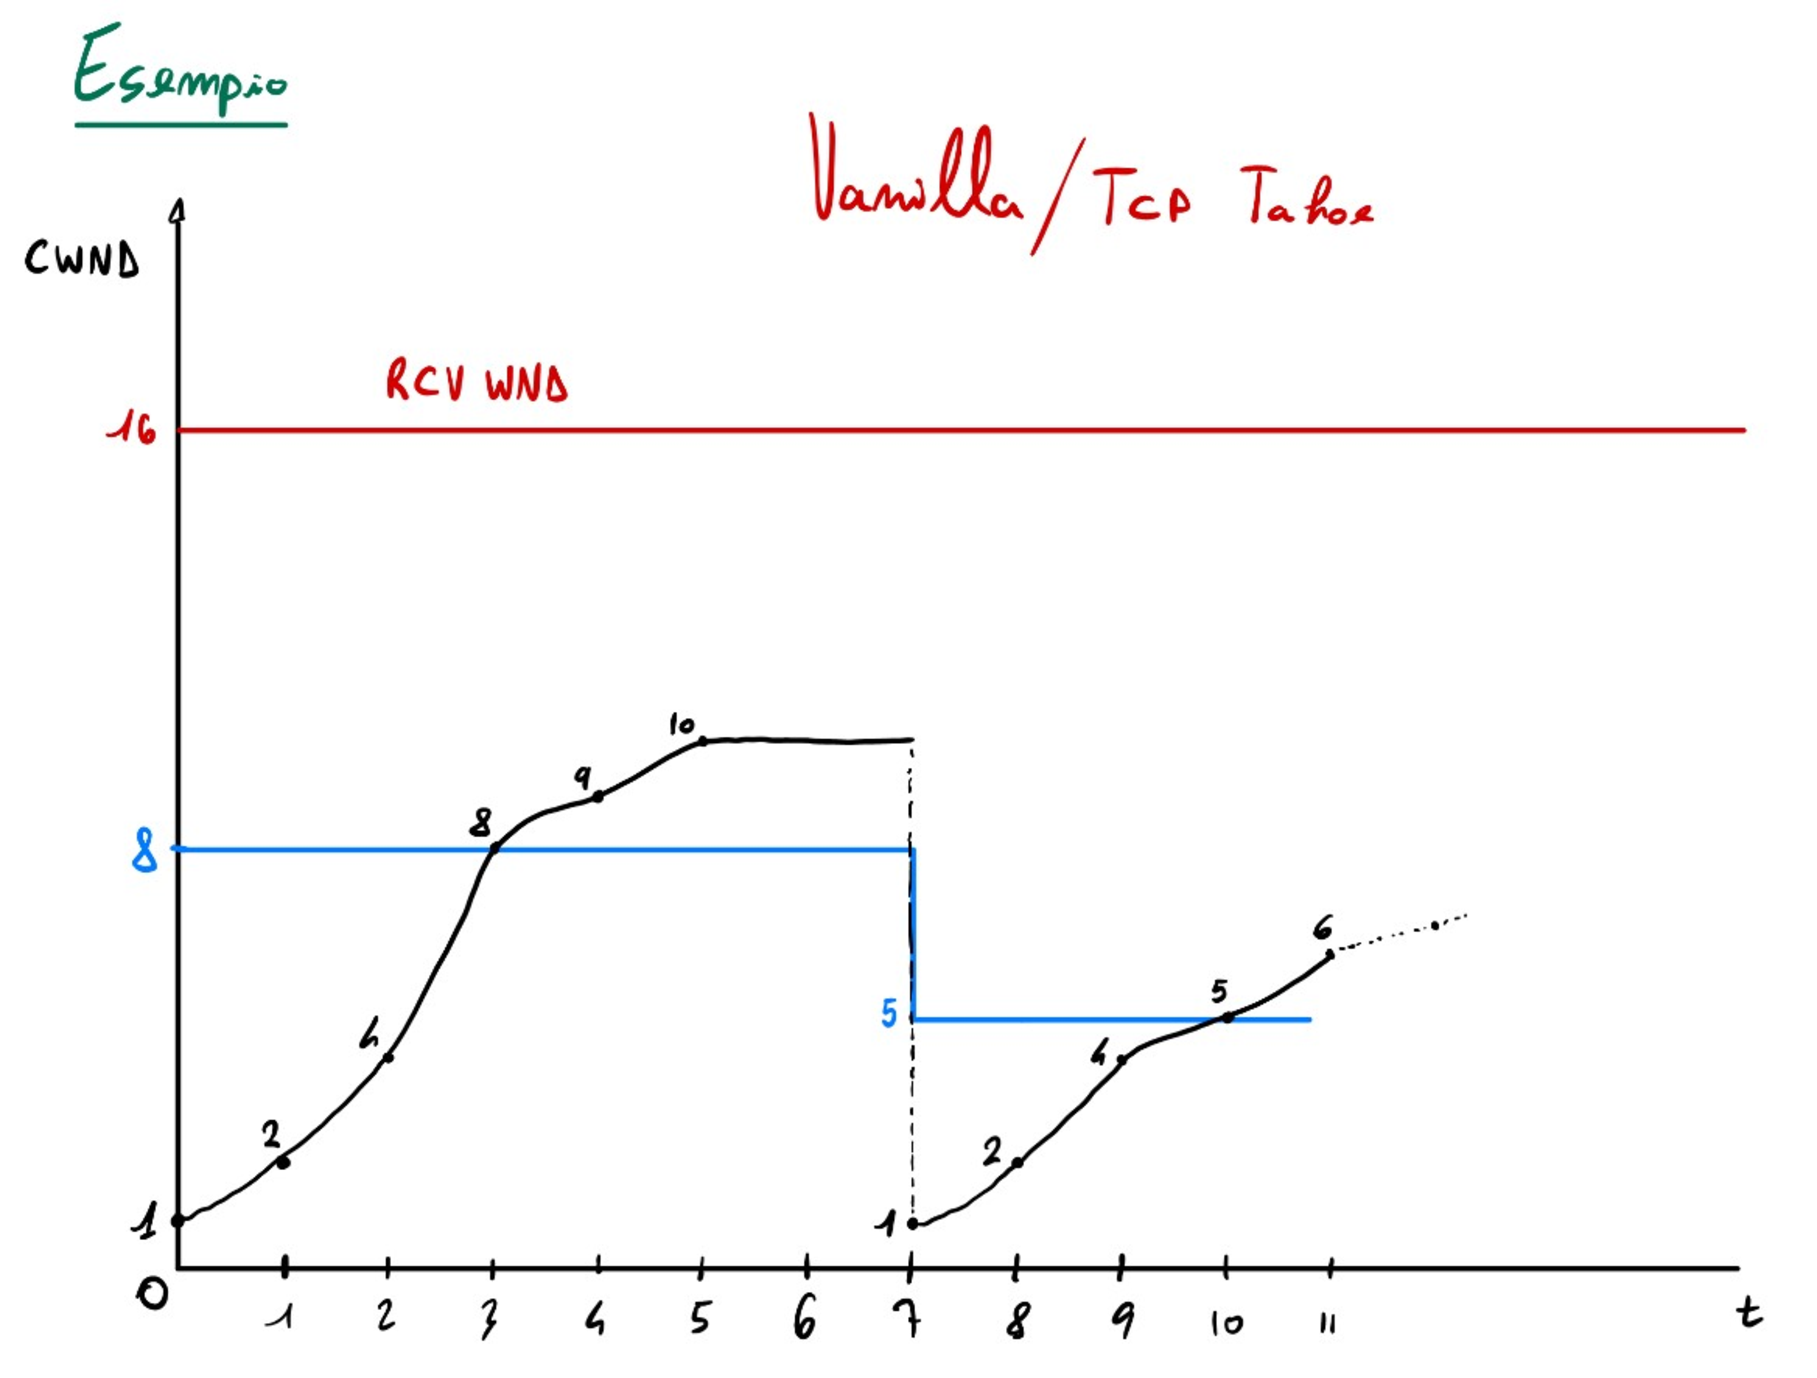
\includegraphics[width=\textwidth]{img/congestione_eg_esercizio.pdf}
	\end{figure}
	
	\noindent
	È interessante notare la differenza nel caso in cui si utilizzi la versione di TCP Reno, ovvero la più recente. Essa utilizza la \emph{Fast Recovery}, una tecnica spiegata nel capitolo precedente. L’andamento è molto variabile e qui di seguito si rappresenta con un grafico approssimativo.
	\begin{figure}[!htp]
		\centering
		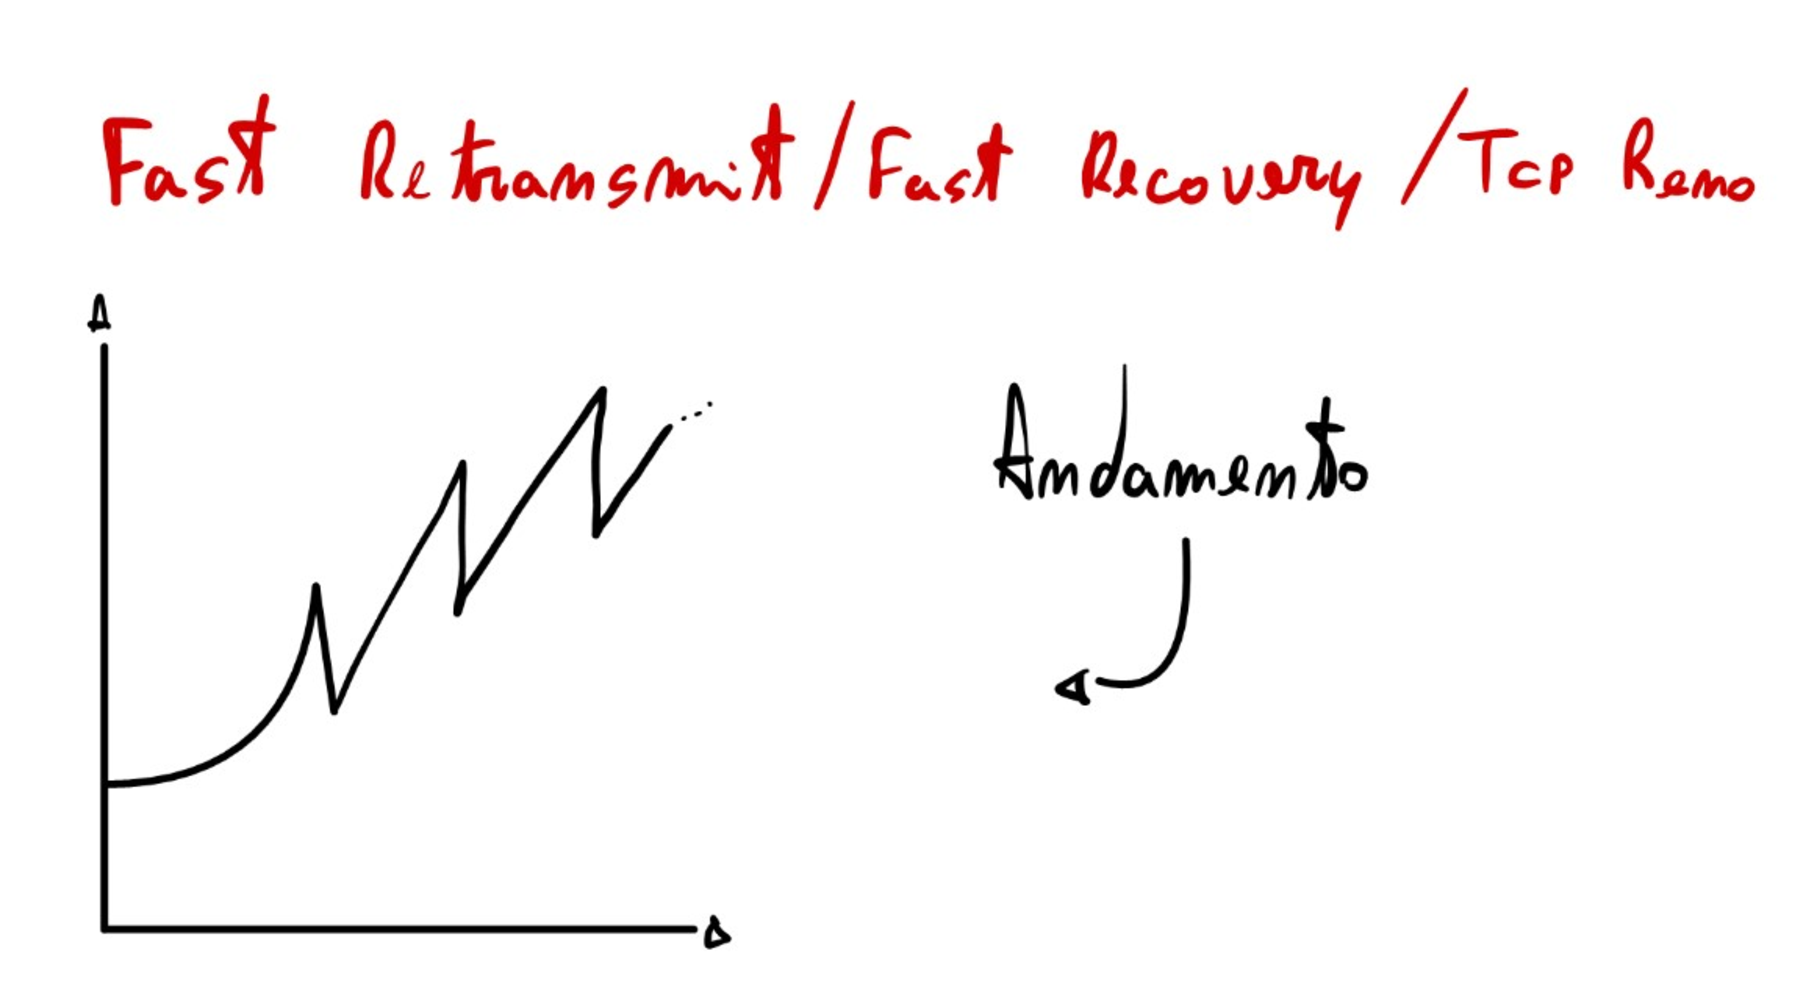
\includegraphics[width=.8\textwidth]{img/andamento.pdf}
	\end{figure}\newpage

	\subsection{\textcolor{Red3}{Esercizio sul controllo della congestione TCP}}
	
	\subsubsection{\textcolor{Red3}{Esercizio 1}}
	
	L’applicazione A deve trasferire all’applicazione B $96'000$ Byte. La connessione è già stata instaurata. I dati disponibili sono:
	\begin{itemize}
		\item $\textsf{MSS} = 1'000$ Byte
		\item $\textsf{RCV WND} = 32'000$ Byte costante
		\item $\textsf{SSTHRESH} = \textsf{RCV WND} \div 2$
		\item $\textsf{RTT} = 0,50$ secondi costante
		\item $\textsf{RTO} = \textsf{RTT} \times 2$ e raddoppia in caso di perdite sequenziali
	\end{itemize}
	Infine, negli intervalli aperti $3 - 3.5$ e $7 - 7.5$ è presente un down di rete.\newline
	
	\noindent
	Il \textbf{primo passo} per risolvere l’esercizio è la numerazione dei segmenti. Per farlo basta prendere il numero dei Byte da trasferire e dividere il valore per la \textsf{MSS}:
	\begin{equation*}
		\textbf{Numero di segmenti da inviare } \longrightarrow 96'000 \div 1'000 = 96 \text{ segmenti}
	\end{equation*}
	Prima di passare al secondo passaggio e osservare il numero di segmenti da inviare, è necessario ottenere il valore della \textsf{RCV WND} (finestra massima di ricezione) per avere conseguentemente anche la \textsf{CWND}. Essa è possibile calcolarla facendo una semplice divisione tra il numero di Byte della \textsf{RCV WND} e della \textsf{MSS}:
	\begin{equation*}
		\textbf{\textsf{RCV WND} } \longrightarrow 32'000 \div 1'000 = 32 \text{ segmenti}
	\end{equation*}
	E la \textsf{SSTHRESH}, come scritto nei dati del testo dell’esercizio, è ottenibile dividendo per due la \emph{receive window}:
	\begin{equation*}
		\textbf{\textsf{SSTHRESH} } \longrightarrow 32 \div 2 = 16 \text{ segmenti}
	\end{equation*}\newpage
	\noindent
	Il \textbf{secondo passo} necessita di uno schema. Esso ha nell'asse delle ascisse ($x$) il tempo e nell'asse delle ordinate ($y$) la \textsf{CWND}.
	\begin{figure}[!htp]
		\centering
		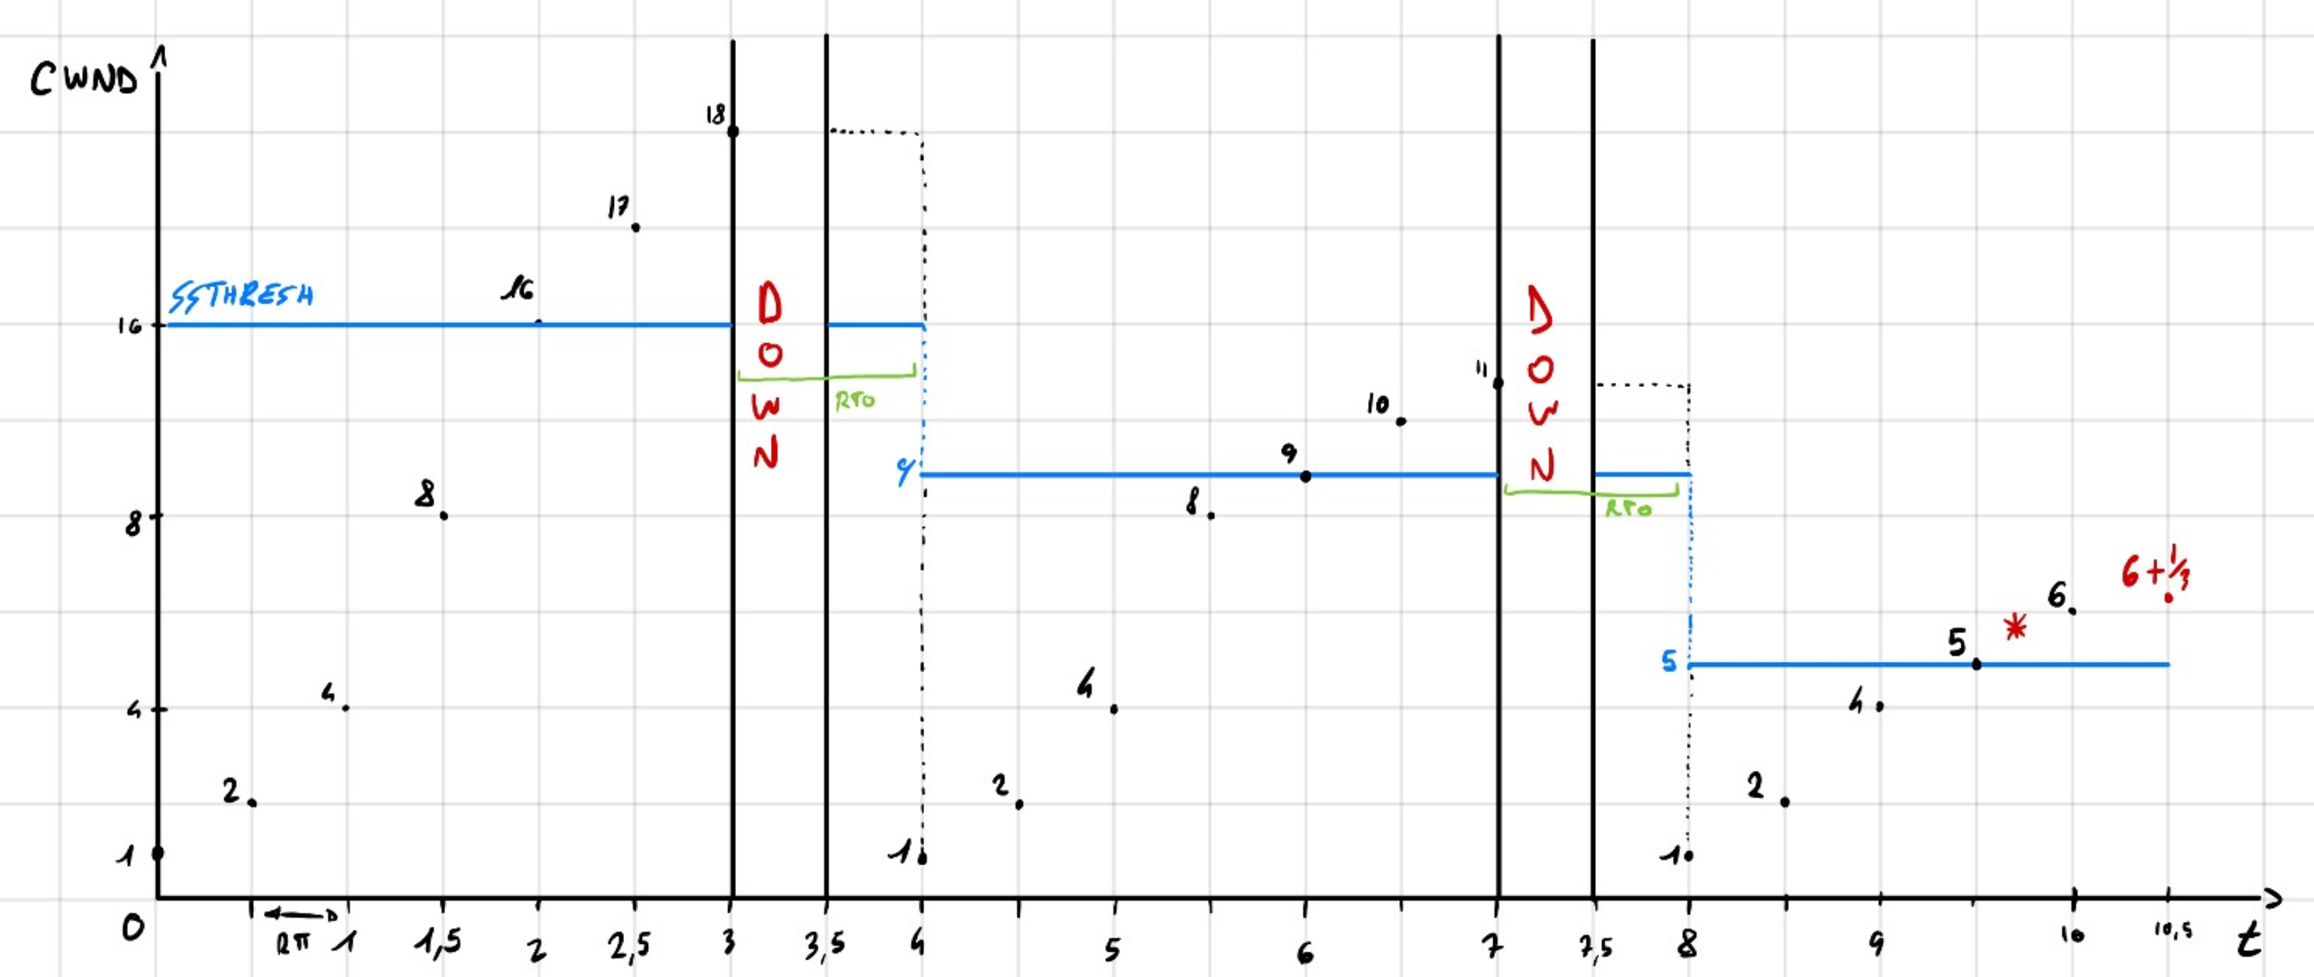
\includegraphics[width=\textwidth]{img/ex1_congestione.pdf}
	\end{figure}
	
	\noindent
	All’inizio i pacchetti trasmessi seguono l’algoritmo slow start e c’è poco da dire. La somma dinamica, ovvero la somma dei segmenti inviati con successo necessaria per capire quando concludere la connessione, al tempo $t_{1,5}:1+2+4+8=15$.\newline
	
	\noindent
	Successivamente la \textsf{CWND} diventa come la \textsf{SSTHRESH} e l’avanzata diventa più cauta, notabile all’aumento di 1 valore per volta dal tempo $t_{2}$ fino al tempo $t_{3}$.\newline
	
	\noindent
	A questo punto, l’\textbf{evento down} non permette ai 18 \emph{segmenti} di giungere correttamente a destinazione. Il protocollo TCP, alla fine del RTO entra nella fase di recupero del segmento perso: la \textsf{SSTHRESH} viene posta a 9 ($\textsf{CWND} \div 2 \rightarrow 18 \div 2$), la nuova $\textsf{CWND}_{new} = 1$ e il nuovo $\textsf{RTO}_{new} = \textsf{RTO} \times 2$. Dato che l’\textsf{RTO} è ad 1 perché $0,5 \cdot \left(\textsf{RTT}\right) \times 2$, all’incirca al tempo $t_{4}$ riparte la fase di \emph{slow start}.\newline
	
	\noindent
	\textbf{Attenzione!} Nella somma dinamica, i 18 \emph{segmenti} persi non vengono contati e quindi il risultato fino al tempo $t_{3}$ è $1+2+4+8+16+17\cancel{+18}=48$.\newline
	
	\noindent
	Questo evento di \emph{down} si ripete anche al tempo $t_{7}$.\newline
	
	\noindent
	L'\textbf{ultimo passo} è la fase di chiusura della connessione. Al tempo $t_{10}$ la \textsf{CWND} viene posta a 6 come impone l'algoritmo. Effettuando la somma dinamica si ha come risultato:
	\begin{equation*}
		1+2+4+8+16+17+1+2+4+8+9+10+1+2+4+5=94
	\end{equation*}
	Se i segmenti inviati sono 94, ne servono 2 per giungere a 96, ovvero all’obbiettivo dell’esercizio. Quindi, al tempo $t_{10}$ vengono inviati 2 segmenti nonostante la grandezza della \textsf{CWND} è posta a 6. A questo punto, una volta ricevuti gli ultimi \textsf{ACK} dei segmenti inviati, al tempo $t_{10,5}$ (dopo mezzo secondo perché \textsf{RTT} è di $0,50$ secondi) è possibile chiudere la connessione.\newline
	
	\noindent
	La chiusura avviene dunque al tempo $t_{10,5}$ con l’aggiornamento della \textsf{CWND}: la \textsf{CWND} è maggiore della \textsf{SSTHRESH}, il valore minimo da scegliere sarà $\frac{\textsf{CWND}_{old} + \left(\text{\#ack ricevuti}\right)}{\textsf{CWND}_{old}}$  (e non la \textsf{RCV WND}), ovvero $6+\frac{2}{6}$. \textbf{Solo dopo aver aggiornato la \textsf{CWND}, la connessione si può dire conclusa}.\newpage
	
	\subsubsection{\textcolor{Red3}{Esercizio 2}}
	
	L’applicazione A trasferisce $46'500$ Byte all’applicazione B. I dati sono:
	\begin{itemize}
		\item $\textsf{MSS} = 1'500$ Byte
		\item $\textsf{RCV WND} = 24'000$ Byte costante
		\item $\textsf{SSTHRESH}_{iniziale} = \textsf{RCV WND}_{iniziale} \div 2$
		\item $\textsf{RTT} = 0,50$ secondi costante
		\item $\textsf{RTO} = \textsf{RTT} \times 2$ e raddoppia in caso di perdite consecutive
	\end{itemize}
	Infine, gli eventi che si manifestano sono due \emph{down} di rete al tempo $1,5 - 3,5$ e $7 - 7,5$.\newline
	
	\noindent
	Il \textbf{primo passo} è l'enumerazione dei segmenti da inviare:
	\begin{equation*}
		\text{dati da inviare} \div \textsf{MSS} = 46'500 \div 1'500 = 31 \text{ segmenti}
	\end{equation*}
	E il calcolo della \textbf{SSTHRESH} partendo dalla \textsf{RCV WND}:
	\begin{equation*}
		\begin{array}{lll}
			\textbf{\textsf{RCV WND}} 	& = & 24'000 \div 1'500 = 16 \text{ segmenti} \\
			\textbf{\textsf{SSTHRESH}} 	& = & \textsf{RCV WND} \div 2 = 16 \div 2 = 8 \text{ segmenti}
		\end{array}
	\end{equation*}\newpage
	\noindent
	E adesso si lascia qui di seguito il grafico contenente l’andamento della CWND e del resto:
	\begin{figure}[!htp]
		\centering
		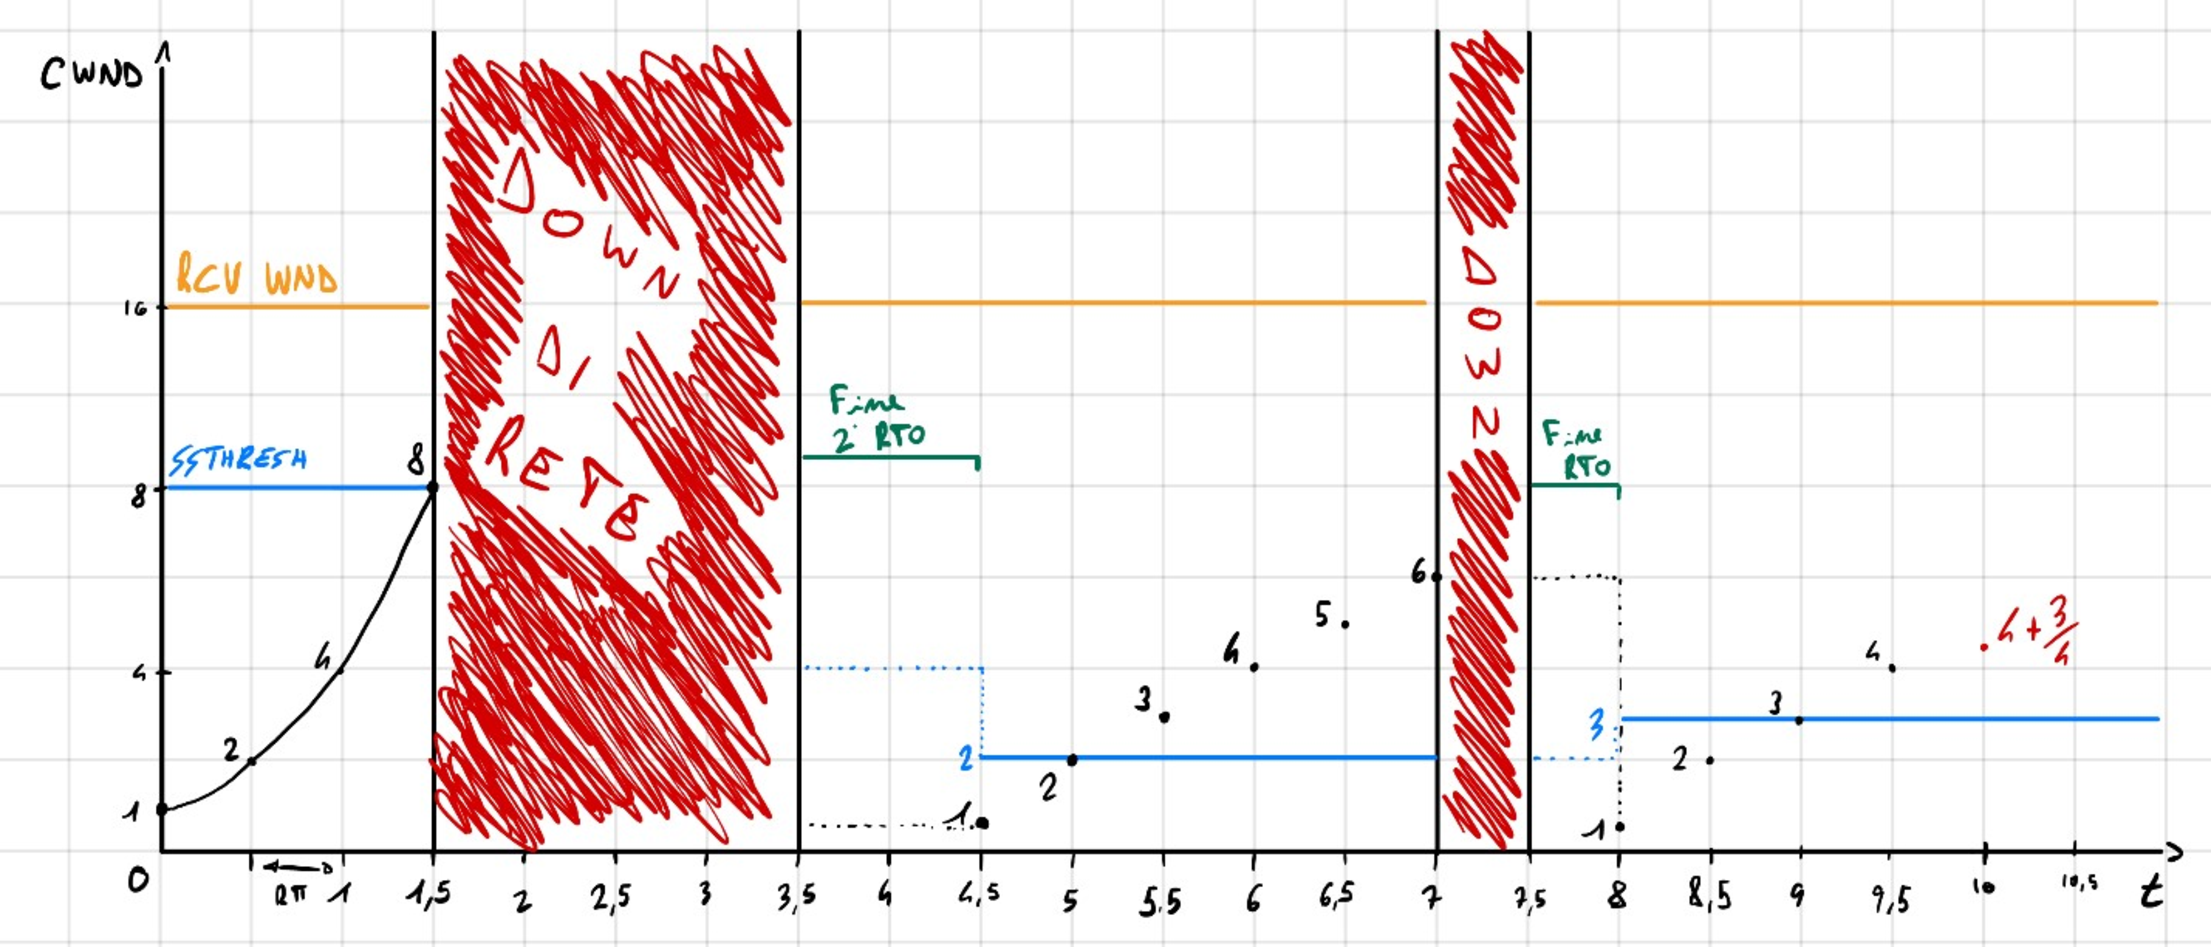
\includegraphics[width=\textwidth]{img/ex2_congestione.pdf}
	\end{figure}

	\noindent
	Ci sono solo due osservazioni importanti degne di nota. La \underline{prima} riguarda il primo down di rete. Al tempo $t_{2,5}$, il TCP del mittente A non riceve i riscontri dei segmenti inviati e viene dunque dimezzata la \textsf{SSTHRESH} ($\textsf{CWND} \div 2$), la \textsf{CWND} riparte da 1 e \textsf{RTO} diventa il doppio, quindi da 1 passa a 2. La parte interessante è questa: alla fine del secondo \textsf{RTO} (tempo $t_{4,5}$), il TCP del mittente non ha ancora ricevuto i pacchetti, per cui dovrebbe diminuire \emph{di nuovo} la \textsf{SSTHRESH} dividendo la \textsf{CWND} per due. Tuttavia, dato che la \textsf{CWND} è al valore minimo, non avrebbe senso portare la \textsf{SSTHRESH} a $0,5$, per cui si imposta il \textbf{valore minimo} della \textsf{SSTHRESH} che corrisponde a 2.\newline
	
	\noindent
	A questo punto inizia l’algoritmo di \emph{slow start} e l’invio dei pacchetti.\newline
	
	\noindent
	La \underline{seconda osservazione} riguarda la chiusura della connessione che non necessita di commenti particolari ma di una piccola precisazione per comprendere meglio. Al tempo $t_{9,5}$ vengono inviati 3 segmenti nonostante la \textsf{CWND} sia di 4. Questo accade poiché ne mancavano soltanto 3 al conteggio finale.\newpage
	
	\section{Protocollo IP}
	
	\subsection{Definizione}
	
	A \textbf{livello di rete} esiste un altro protocollo, chiamato \textcolor{Red3}{\textbf{protocollo IP}} (\emph{Internet Protocol}). Esso fornisce una comunicazione logica tra gli host.\newline
	
	\noindent
	Il protocollo IP non fornisce \textbf{nessuna garanzia di consegna del messaggio} e per questo motivo il servizio viene chiamato \emph{best-effort delivery service}, o abbreviato in \textbf{\emph{best-effort}} (tradotto in \dquotes{massimo sforzo}). In partole povere, il protocollo IP si impegna a finché il messaggio venga consegnato, ma non offre garanzie sulla buona riuscita. Quindi \textbf{non vengono garantiti}:
	\begin{itemize}
		\item Consegna dei segmenti;
		\item Rispetto dell'ordine originario;
		\item Integrità dei dati all'interno dei segmenti.
	\end{itemize}
	Per cui, si conclude che il \textbf{protocollo IP} è un \underline{\textbf{servizio \emph{non} affidabile}}. Nonostante l'inaffidabilità del protocollo, quest'ultimo ha una motivazione solida per essere tale: il protocollo di trasporto, TCP o UDP, si occupa dell'affidabilità. Per cui sarebbe ridondante avere due livelli che si preoccupano di questa caratteristica.\newpage
	
	\subsection{Formato dei datagrammi (IPv4)}\label{ipv4}
	
	Come detto nei capitoli precedenti, il pacchetto a livello di rete viene chiamato \textcolor{Red3}{\textbf{datagramma}}. Il formato dei datagrammi IPv4 è mostrato qui di seguito:
	
	\begin{figure}[!htp]
		\centering
		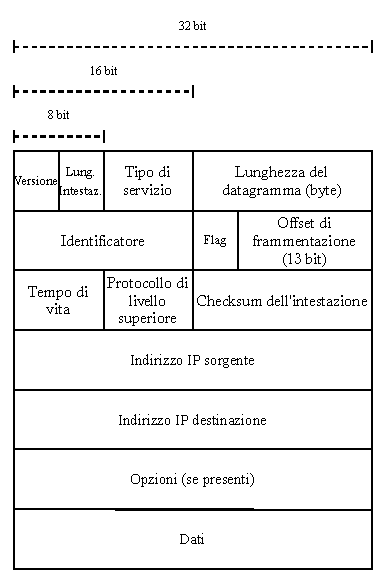
\includegraphics[width=.85\textwidth]{img/datagrammi_ipv4.pdf}
		\caption{Formato dei datagrammi nella versione IPv4.}
	\end{figure}

	\newpage\noindent
	L'\textbf{intestazione} (\emph{header}) è formato da 20 byte (escluso \dquotes{Opzioni}) e include:
	\begin{itemize}
		\item $\left[4\text{ bit}\right]$ \underline{\textbf{Numero di versione}} (\emph{version}). Questo campo specifica la versione del protocollo IP del datagramma, consentendo al router la corretta interpretazione del datagramma. È importante la sua presenza poiché esistono un po' di versioni del protocollo IP, la più famosa è IPv4 (attualmente la più usata) e IPv6 (ancora semi-inutilizzata).
		
		\item $\left[4\text{ bit}\right]$ \underline{\textbf{Lunghezza dell'intestazione}} (\emph{header length}). Il campo \dquotes{Opzioni} può contenere un numero non definito a priori di informazioni. Questo campo indica dove iniziano effettivamente i dati del datagramma. Nel caso in cui \dquotes{Opzioni} non fosse presente, come nella maggior parte dei casi, l’intestazione avrà una lunghezza di 20 byte.
		
		\item $\left[8\text{ bit}\right]$ \underline{\textbf{Tipo di servizio}} (\emph{type of service}, TOS). Questo campo indica i diversi tipi di datagrammi. Per esempio, datagrammi in tempo reale (usati nella telefonia), datagrammi da altro traffico (per esempio, FTP).
		
		\item $\left[16\text{ bit}\right]$ \underline{\textbf{Lunghezza del datagramma}} (\emph{total length}, TL). Rappresenta la lunghezza totale del datagramma, quindi intestazione più dati, misurata in byte. Dato che la massima lunghezza di questo campo è 16 bit, la massima dimensione dei datagrammi IP è $65'535$ byte.
		
		\item $\left[16\text{ bit}, 3\text{ bit}, 13\text{ bit}\right]$ \underline{\textbf{Identificatore}}, \underline{\textbf{flag}}, \underline{\textbf{offset di frammentazione}} (\emph{identification, flag, fragment offset}). Questi tre campi vengono impiegati nella frammentazione (trattato nei prossimi capitoli). Attenzione! La versione IPv6 non consente frammentazione sui router.
		
		\item $\left[8\text{ bit}\right]$ \underline{\textbf{Tempo di vita}} (\emph{time-to-live}, TLL). Questo campo è incluso poiché ha l’obbiettivo di assicurare che i \textbf{datagrammi non restino in circolazione per sempre nella rete} a causa, per esempio, di un instradamento ciclico. Per evitare ciò, viene decrementato il tempo di vita di un’unità ogni volta che il datagramma è elaborato da un router; quando viene raggiunto il valore 0, il datagramma viene scartato.
		
		\item $\left[8\text{ bit}\right]$ \underline{\textbf{Protocollo}} (\emph{protocol}). Questo campo viene utilizzato solitamente dal destinatario ed indica lo specifico protocollo a livello di trasporto al quale vanno passati i dati del datagramma. Per esempio, il valore 6 indica che i dati sono destinati a TCP, mentre il valore 17 indica che i dati sono destinati a UDP. In altre parole, il numero di protocollo è l’anello di collegamento tra i livelli di rete e di trasporto, mentre il numero di porta è il \dquotes{collante} che lega i livelli di trasporto e di applicazione.
		
		\item $\left[16\text{ bit}\right]$ \underline{\textbf{Checksum dell'intestazione}} (\emph{header checksum}). Il checksum viene calcolato dal mittente, ricalcolato e aggiornato ad ogni router (come anche il campo TTL e i campi \dquotes{Opzione}) e ricalcolato dal destinatario per verificare che non si siano manifestati errori. Il calcolo viene effettuato tramite alcuni algoritmi.
		
		\item $\left[32\text{ bit}, 32\text{ bit}\right]$ \underline{\textbf{Indirizzo IP sorgente e destinazione}} (\emph{source address, destination address}). L'indirizzo IP sorgente e destinazione vengono inseriti dal mittente nel momento in cui viene creato il datagramma.
		
		\item $\left[\text{undefined bit}\right]$ \underline{\textbf{Opzioni}} (\emph{option}). I bit di opzioni formano più campi e variano a seconda delle necessità. L’obbiettivo è quello di estendere l’intestazione IP, tuttavia questo insieme di campi crea svariati problemi. A causa dei seguenti ostacoli, nella nuova versione IPv6 si è deciso di rimuoverlo:
		\begin{itemize}
			\item A causa della \textbf{lunghezza variabile} non è possibile determinare a priori dove comincerà il campo dati;
			
			\item Nel caso in cui il datagramma abbia bisogno di \textbf{elaborare} i campi opzioni, il \textbf{tempo necessario} per questa operazione su un router \textbf{può variare} in modo significativo.
		\end{itemize}
	\end{itemize}
	Invece, il campo \textbf{dati} (\emph{payload}) contiene il segmento a livello di trasporto (TCP o UDP) da consegnare alla destinazione. Tuttavia, può trasportare anche altri tipi di dati, quali i messaggi ICMP (\href{https://en.wikipedia.org/wiki/Internet_Control_Message_Protocol}{\emph{Internet Control Message Protocol}}).\newpage
	
	\section{Frammentazione dei datagrammi IPv4}
	
	\subsection{Definizione}
	
	Non tutti i protocolli possono trasportare pacchetti della stessa dimensione a livello di rete. Per esempio, i frame Ethernet possono trasportare fino a $1500$ byte di dati, mentre i frame di alcuni collegamenti su grandi distanze non possono trasportare più di $576$ byte.\newline
	
	\noindent
	Per usare una terminologia corretta, si definisce \textcolor{Red3}{\textbf{unità massima di trasmissione}} (MTU, \emph{maximum transmission unit}) la \textbf{massima quantità di dati} che un frame a livello di collegamento può trasportare. La MTU può essere diversa a seconda della tratta, o percorso, che percorrono i frame e dunque diventa un limite legato ai differenti protocolli utilizzati a livello di collegamento.\newline
	
	\noindent
	La soluzione a questo limite è la tecnica della \textcolor{Red3}{\textbf{frammentazione dei pacchetti}}. Quindi, frammentare letteralmente i dati del datagramma IP in due o più datagrammi IP più piccoli, chiamati \textbf{frammenti}, e quindi trasferiti sul collegamento di uscita.
	
	\subsection{Fasi della frammentazione}
	
	Le fasi della frammentazione sono 5:
	\begin{enumerate}[label=\Roman*.]
		\item \textbf{\underline{Creazione datagramma}}. Durante la creazione, l’host contrassegna il datagramma con un numero identificativo e con gli indirizzi di sorgente e destinazione.
		
		\item \textbf{\underline{Frammentazione datagramma}}. Il router frammenta il datagramma, contrassegna i frammenti con gli indirizzi di sorgente e di destinazione e con l’identificatore numerico del datagramma originario.
		
		\item \textbf{\underline{Ricezione datagrammi}}. Una volta che il destinatario riceve una serie di datagrammi dello stesso host mittente, può esaminare gli identificatori per individuare i frammenti di uno stesso datagramma.
		
		\item \textbf{\underline{Flag di terminazione}}. Per far sì che il destinatario riesca a riassemblare i frammenti, si utilizza il campo flag \textsf{M} per indicare con 0 l’ultimo frammento di un frame e 1 un frammento intermedio di un frame.
		
		\item \textbf{\underline{Campo di offset}}. Il campo di offset viene utilizzato per specificare l’esatto ordine che i frammenti avevano originariamente all’interno del datagramma IP e per determinare se un frammento è stato perduto.
	\end{enumerate}
	Quindi, i \textbf{campi utilizzati} durante la frammentazione sono: \textbf{Identificatore} (\emph{Identification}), \textbf{Offset di frammentazione} (\emph{Fragment Offset}) e \textbf{Flag M}. Il primo è un numero progressivo dato dalla sorgente ad ogni pacchetto, il secondo identifica la posizione del pacchetto rispetto a quello originale (di default il valore è $000$ e solitamente viene diviso per $8$) e l'ultimo, come dice il punto 4, indicare se il frammento è l'ultimo o l'intermedio.
	\newpage

	\subsection{\textcolor{Red3}{Esercizio sul controllo della congestione TCP}}
	
	L’applicazione A deve trasferire all'applicazione B $104'000$ Byte. La connessione è già stata instaurata. I dati disponibili sono:
	\begin{itemize}
		\item $\textsf{MSS} = 1'200$ Byte
		\item $\textsf{RCV WND} = 24'000$ Byte costante
		\item $\textsf{SSTHRESH} = \textsf{RCV WND}$
		\item $\textsf{RTT} = 0,50$ secondi costante
		\item $\textsf{RTO} = \textsf{RTT} \times 2$ e raddoppia in caso di ritrasmissioni
	\end{itemize}
	Infine, negli intervalli $3.5 - 4$ e $6.5 - 10.5$ è presente un \emph{down} di rete.\newline
	
	\noindent
	Il \textbf{primo passo} per risolvere l'esercizio è la numerazione dei segmenti da inviare. Per farlo basta prendere il numero dei \emph{Byte} da trasferire e dividere il valore per la \textsf{MSS}:
	\begin{equation*}
		\textbf{Numero di segmenti da inviare } \rightarrow 104'000 \div 1'200 = 87 \emph{ segmenti}
	\end{equation*}
	Prima di passare al secondo passaggio e osservare il numero di segmenti da inviare, è necessario ottenere il valore della \textsf{RCV WND} (finestra massima di ricezione) per avere conseguentemente anche la \textsf{CWND}. Essa è possibile calcolarla facendo una semplice divisione tra il numero di Byte della \textsf{RCV WND} e della \textsf{MSS}:
	\begin{equation*}
		\textbf{\textsf{RCV WND}} \rightarrow 24'000 \div 1'200 = 20 \emph{ segmenti}
	\end{equation*}
	E la \textsf{SSTHRESH}, come scritto nei dati del testo dell'esercizio, è uguale alla \emph{receive window}:
	\begin{equation*}
		\textsf{\textbf{SSTHRESH}} \rightarrow 20 \emph{ segmenti}
	\end{equation*}\newpage

	\noindent
	Il \textbf{secondo passo} necessita di uno schema. Esso ha nell'asse delle ascisse ($x$) il tempo e nell'asse delle ordinate ($y$) la \textsf{CWND}.
	\begin{figure}[!htp]
		\centering
		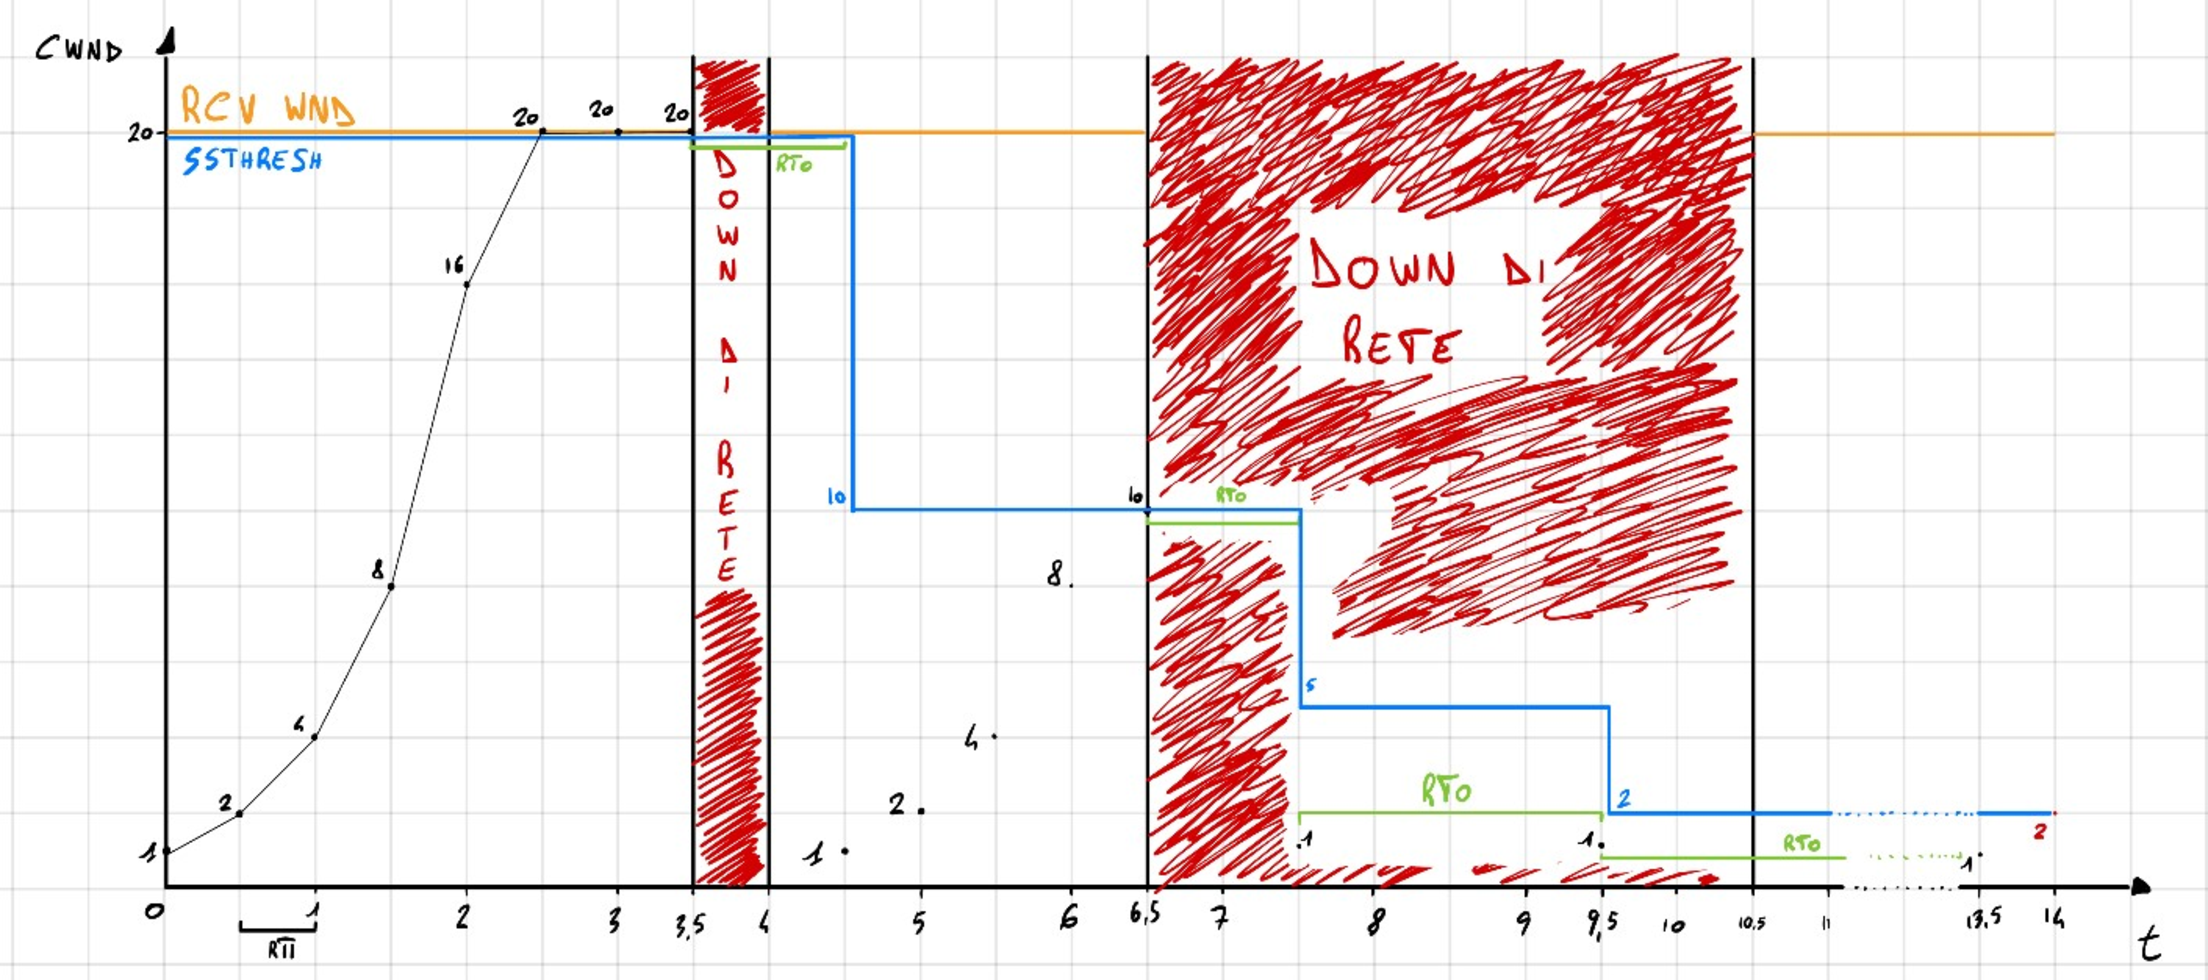
\includegraphics[width=\textwidth]{img/ex3_congestione.pdf}
	\end{figure}

	\noindent
	All’inizio i pacchetti trasmessi seguono l’algoritmo \emph{slow start} e c’è poco da dire. La somma dinamica, ovvero la somma dei segmenti inviati con successo, è necessaria per capire quando concludere la connessione. Al tempo $t_{2}$ la situazione è la seguente: $t_{2} : 1+2+4+8+16 = 31$.\newline
	
	\noindent
	Successivamente la \textsf{CWND} diventa come la \textsf{SSTHRESH} e la \textsf{RCVWND}, quindi fermo al valore $20$ dal tempo $2,5$ al tempo $3,5$ (tempo in cui si manifesta il \emph{down} di rete tra l’altro).\newline
	
	\noindent
	A questo punto, l’\textbf{evento \emph{down}} non consente ai $20$ \emph{segmenti} di giungere correttamente a destinazione. Il protocollo TCP, alla fine del \textsf{RTO} \textbf{entra nella fase di recupero del segmento perso}: la \textsf{SSTHRESH} viene posta a $10$ ($\textsf{CWND} \div 2 \rightarrow 20 \div 2$), la nuova $\textsf{CWND}_{new} = 1$ e il nuovo $\textsf{RTO}_{new} = \textsf{RTO} \times 2$. Dato che l’\textsf{RTO} è ad $1$ poiché $0,5 \cdot \left(\textsf{RTT}\right) \cdot 2$, all’incirca al tempo $t_{4,5}$ riparte la fase di \emph{slow start}.\newline
	
	\noindent
	\textbf{\underline{Attenzione!}} Nella somma dinamica, i $20$ segmenti persi non vengono contati e quindi il risultato fino al tempo $t_{3,5}$ è $1+2+4+8+16+20+20\cancel{+20}=71$.\newline
	
	\noindent
	Questo evento di \emph{down} si ripete anche al tempo $t_{6,5}$. In questo caso, l’\textsf{RTO} scade e il mittente ritenta un nuovo tentativo impostando la nuova $\textsf{CWND}_{new} = 1$, la \textsf{SSTHRESH} alla metà, cioè $5$, e il nuovo $\textsf{RTO}_{new} = \textsf{RTO} \times 2$, cioè $\textsf{RTO}_{new} = 1 \times 2 = 2$. Ancora una volta, \textbf{il mittente non riesce a consegnare il pacchetto}, per cui: la \textsf{CWND} diminuisce nuovamente ma dato che era a $1$, rimane tale $\textsf{CWND}_{new}=1$; la \textsf{SSTHRESH} diminuisce della metà $5 \div 2 = 2,5$ (ignorando il resto nella divisione, quindi si considera \textbf{sempre} l'approssimazione per difetto). Infine, viene eseguito un altro tentativo, ma a questo punto l’\textsf{RTO} è talmente ampio che per vedere un nuovo tentativo è necessario andare al tempo $t_{13,5}$, ovvero la fine del \textsf{RTO}.\newpage
	
	\noindent
	L’\textbf{ultimo passo} è la fase di chiusura della connessione. Al tempo $t_{13,5}$ viene inviato l’ultimo segmento che viene confermato con il relativo \textsf{ACK} al tempo $14$:
	\begin{equation*}
		1+2+4+8+16+20+20+1+2+4+8+1=87
	\end{equation*}
	La chiusura avviene dunque al tempo $14$ con l’aggiornamento della \textsf{CWND}: la \textsf{CWND} è maggiore della \textsf{SSTHRESH}, il valore minimo da scegliere sarà dunque $\textsf{CWND}_{old} + \frac{\left(\text{\#ack ricevuti}\right)}{\textsf{CWND}_{old}}$ (e non la \textsf{RCV WND}), ovvero $1+1$. \textbf{Solo dopo aver aggiornato la \textsf{CWND}, la connessione si può dire conclusa}.\newpage
	
	\section{Algoritmi di instradamento}
	
	\subsection{Approccio al problema}
	
	A livello di rete esistono \textbf{due possibili} approcci per affrontare il problema dell'instradamento:
	\begin{enumerate}
		\item \textcolor{Red3}{\textbf{\underline{Controllo locale}}}. Come si vede in figura~\ref{controllo_locale}, l’\textbf{algoritmo di instradamento viene eseguito su ogni singolo router}, all’interno del quale vengono effettuate sia le funzioni di inoltro (piano dei dati, \emph{data plane}) che quelle di instradamento (piano di controllo, \emph{control plane}). Ogni router ha una componente di instradamento che comunica con le componenti di instradamento degli altri router per calcolare la propria tabella di inoltro. Questo approccio di controllo locale per router è stato usato in internet per decenni.
		
		\item \textbf{\underline{Controllo logicamente centralizzato}}. Come si vede nella figura~\ref{controllo_logicamente_centralizzato}, il controller logicamente centralizzato (\emph{logically centralized routing controller}) calcola e distribuisce le tabelle di inoltro che devono essere utilizzate da ogni router.
	\end{enumerate}
	\textbf{\underline{Attenzione!}} Al contrario degli algoritmi di instradamento, gli agenti di controllo \textbf{non interagiscono direttamente tra di loro} e \textbf{non partecipano attivamente all’elaborazione della tabella di inoltro}.
	\begin{figure}[!htp]
		\centering
		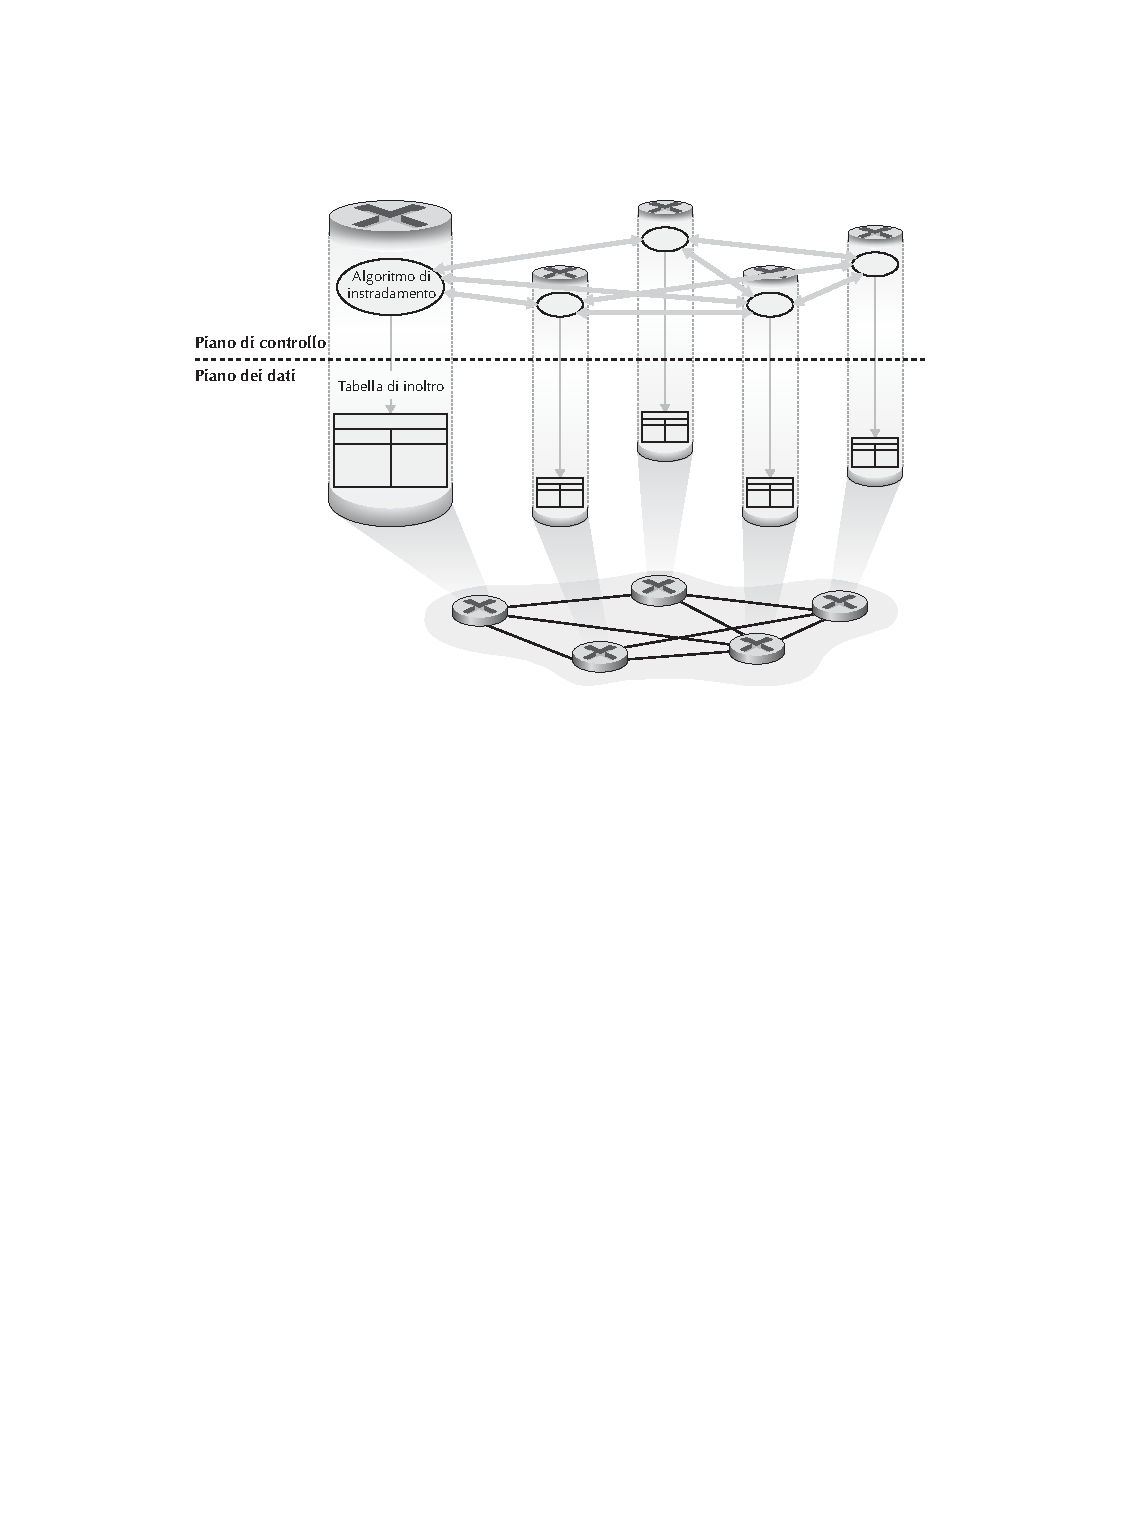
\includegraphics[width=\textwidth]{img/controllo_locale.pdf}\label{controllo_locale}
		\caption{Controllo locale.}
	\end{figure}
	\begin{figure}[!htp]
		\centering
		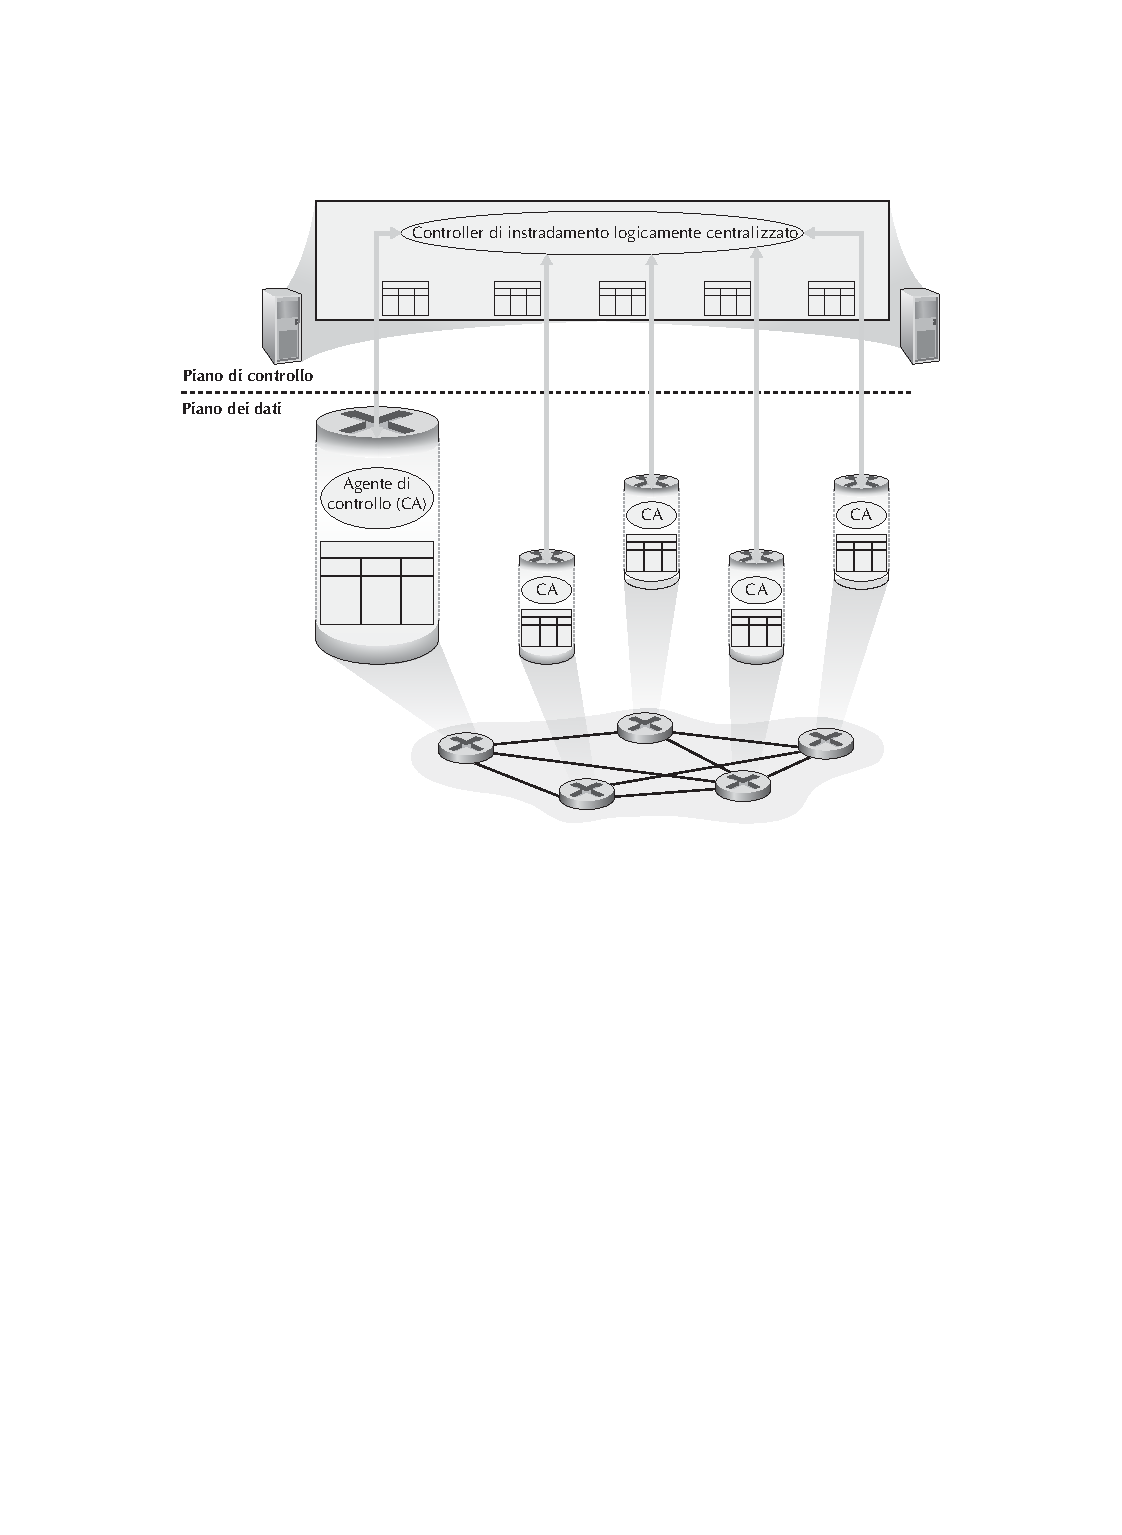
\includegraphics[width=\textwidth]{img/controllo_logicamente_centralizzato.pdf}\label{controllo_logicamente_centralizzato}
		\caption{Controllo logicamente centralizzato.}
	\end{figure}\newpage
	
	\subsection{Algoritmi di instradamento}
	
	Gli \textcolor{Red3}{\textbf{algoritmi di instradamento}} (\emph{routing algorithm}), il cui scopo è determinare i percorsi, o cammini, tra le sorgenti e i destinatari, attraverso la rete di router. Il \underline{percorso migliore} è quello che ha costo minimo, anche se esistono delle problematiche di interesse concreto quali la \emph{policy} (per esempio il router $x$, appartenente all’organizzazione $Y$, non debba inoltrare pacchetti che abbiano come sorgente la rete appartenente all’organizzazione $Z$).\newline
	
	\noindent
	Per \textbf{formulare i problemi di instradamento} si utilizza un \textbf{grafo} $G=\left(N,E\right)$ in cui $N$ rappresentano i nodi ed $E$ rappresentano gli archi (\emph{edge}). Ciascun arco collega una coppia di nodi di $N$. La formulazione prevede:
	\begin{itemize}
		\item I \textbf{nodi} del grafo rappresentano i \emph{router} che prendono decisioni sull’inoltro dei pacchetti;
		
		\item Gli \textbf{archi} che connettono i nodi rappresentano i collegamenti fisici tra i router.
	\end{itemize}
	\begin{figure}[!htp]
		\centering
		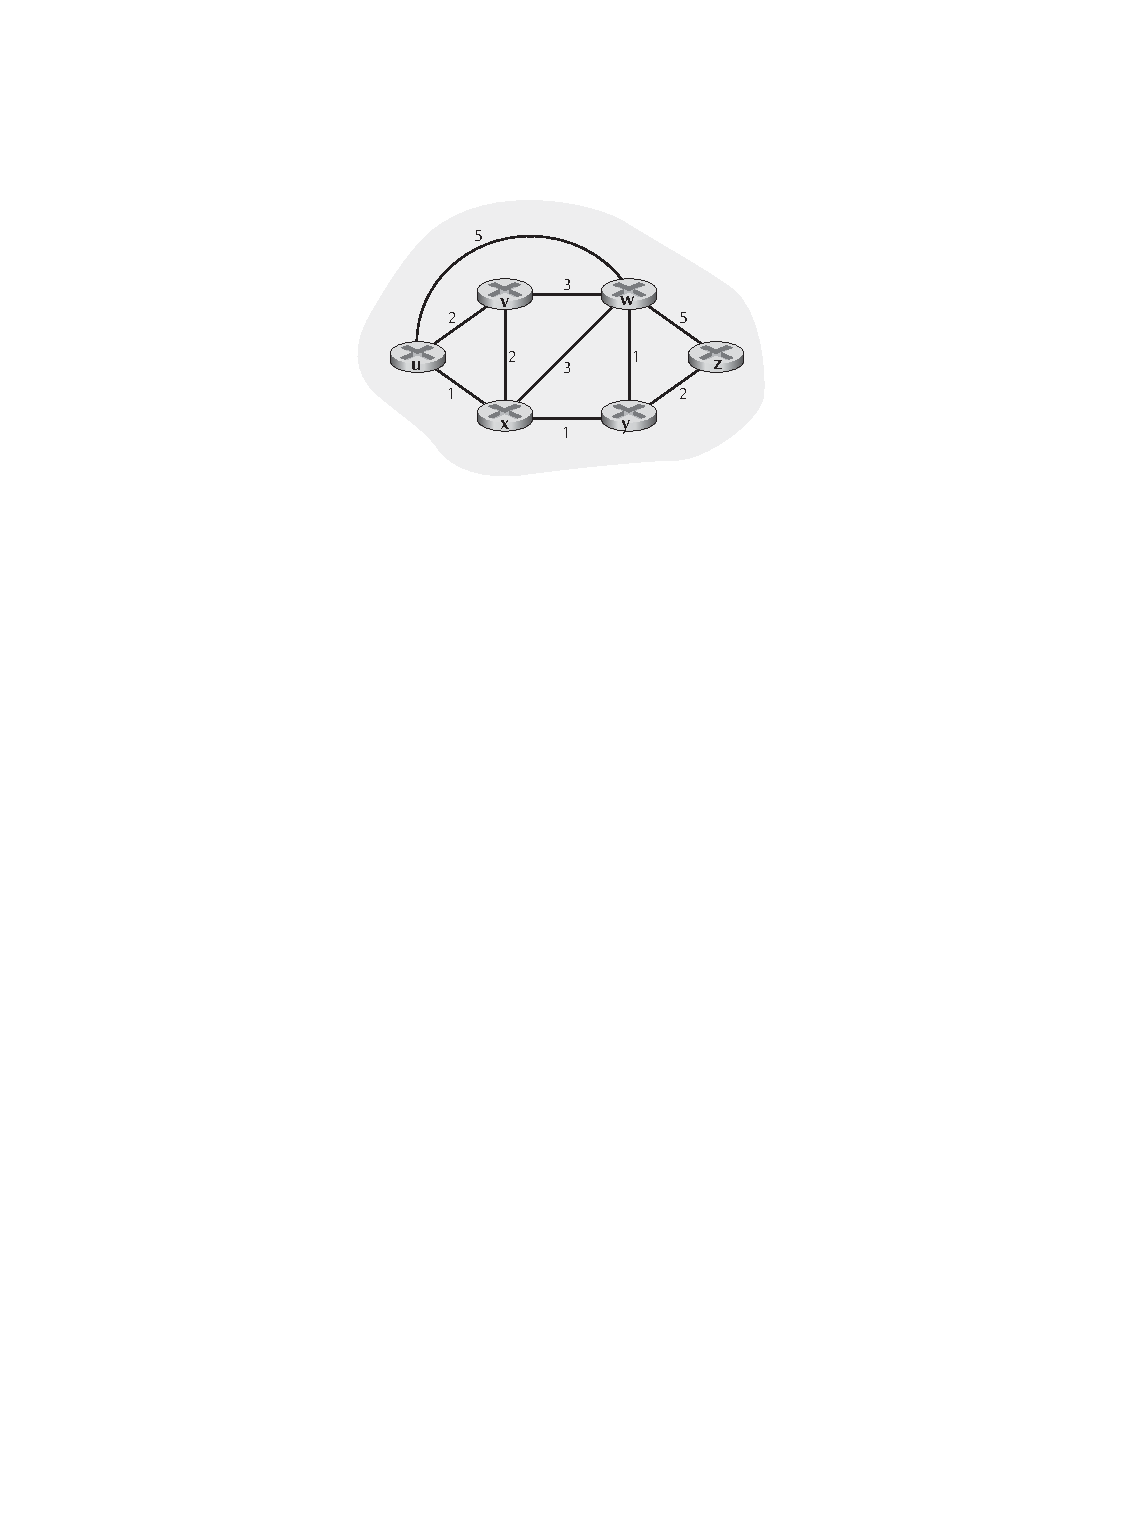
\includegraphics[width=.8\textwidth]{img/eg_grafo_instradamento.pdf}
		\caption{Esempio di grafo.}
	\end{figure}

	\noindent
	Le sue \textbf{proprietà} sono:
	\begin{itemize}
		\item Ad \textbf{ogni arco viene associato un valore che indica il costo}. Quest’ultimo può riflettere la lunghezza fisica del collegamento corrispondente, la velocità del collegamento oppure il suo prezzo;
		\item Si considerano solo \textbf{grafi non orientati}, ovvero con archi bidirezionali;
		\item Un \textbf{nodo} $y$ viene detto \textbf{adiacente o vicino a un altro nodo} $x$ se $\left(x,y\right)$ è un arco in $E$.
	\end{itemize}\newpage

	\noindent
	Le \textbf{notazioni} utilizzate sono:
	\begin{itemize}
		\item Per ogni arco $\left(x,y\right)$ tra i nodi $x$ e $y$ si denota con $c\left(x,y\right)$;
		\item Se la coppia $\left(x,y\right)$ non appartiene a $E$, si denota con $c\left(x,y\right) = +\infty$;
		\item Un \textbf{percorso} in un grafo $G=\left(N,E\right)$ è una sequenza di nodi $\left(x_{1},x_{2},\cdots,x_{n}\right)$ tali che ciascuna delle coppie $\left(x_{1},x_{2}\right)$, $\left(x_{2},x_{3}\right)$, $\cdots$, $\left(x_{p-1},x_{p}\right)$ sia un arco appartenente a $E$.
	\end{itemize}
	
	\noindent
	In generale, gli \textbf{algoritmi di instradamento} sono \textbf{classificati} in due categorie:
	\begin{itemize}
		\item \textbf{Algoritmo di instradamento \underline{centralizzato}} calcola il percorso a costo minimo tra una sorgente e una destinazione avendo una conoscenza globale e completa della rete.\newline
		In altre parole, l’algoritmo riceve in ingresso tutti i collegamenti tra i nodi e i loro costi. Gli algoritmi con informazioni di stato globali sono detti anche \textbf{algoritmi \emph{link-state}} (LS, o con stato del collegamento), dato che l’algoritmo deve essere conscio del costo di ciascun collegamento della rete;
		
		\item \textbf{Algoritmo di instradamento \underline{decentralizzato}}, il percorso a costo minimo viene calcolato in modo distribuito e iterativo. Nessun nodo possiede informazioni complete sul costo di tutti i collegamenti di rete. In questo caso viene studiato l’\textbf{algoritmo \emph{distance-vector}} (DV, o con vettore delle distanze), poiché ogni nodo elabora un vettore di stima dei costi (distanze) verso tutti gli altri nodi n-ella rete.
	\end{itemize}
	
	\noindent
	C’è un \textbf{ulteriore criterio di classificazione}:
	\begin{itemize}
		\item \textbf{Algoritmi di instradamento \underline{statici}} i percorsi vengono cambiati molto raramente, spesso come risultato di un intervento umano (per esempio, la modifica manuale di una tabella di inoltro di un router);
		
		\item \textbf{Algoritmi di instradamento \underline{dinamici}} determinano gli instradamenti al variare del volume di traffico o della topologia della rete.
	\end{itemize}
	
	\noindent
	Un ultimo metodo di classificazione riguardo la \textbf{sensibilità al carico della rete}:
	\begin{itemize}
		\item \textbf{Algoritmo \underline{sensibile al carico}} (\emph{load-sensitive}) i costi dei collegamenti variano dinamicamente per riflettere il livello corrente di congestione;
		
		\item \textbf{Algoritmo \underline{insensibile al carico}} (\emph{load-insensitive}) il costo di un collegamento non riflette esplicitamente il suo attuale (o recente) livello di congestione, per cui non tiene conto di questa sensibilità. Gli algoritmi di instradamento attuali di Internet funzionano in tale modo.
	\end{itemize}
	Infine, esistono \textbf{due tipi di consegne}: \textbf{diretta}, se i due host appartengono alla stessa rete, \textbf{indiretta}. Nel primo caso l'host mittente controlla la propria maschera e i bit del suo prefisso con quello del destinatario. Nel caso in cui sono uguali, allora l'host di destinazione si trova nella stessa rete. Per la consegna indiretta, semplicemente l'host consegna il pacchetto al router.\newpage
	
	\subsection{\textcolor{Red3}{Esercizio sul controllo della congestione TCP}}
	
	L’applicazione A deve trasferire all'applicazione B $104'000$ Byte. La connessione è già stata instaurata. I dati disponibili sono:
	\begin{itemize}
		\item $\textsf{MSS} = 1'200$ Byte
		\item $\textsf{RCV WND} = 9'600$ Byte costante
		\item $\textsf{SSTHRESH} = \textsf{RCV WND}$ iniziale
		\item $\textsf{RTT} = 1$ secondo costante
		\item $\textsf{RTO} = \textsf{RTT} \times 2$ e raddoppia in caso di perdite consecutive
	\end{itemize}
	Infine, nell'intervallo aperto $11.5 - 12.5$ è presente un \emph{down} di rete. Inoltre:
	\begin{itemize}
		\item A partire da $t_{A} > 4.0$ la destinazione annuncia una $\textsf{RCV WND} = 14'400$ Byte;
		\item A partire da $t_{B} > 9.0$ la destinazione annuncia una $\textsf{RCV WND} =  7'200$ Byte.
	\end{itemize}
	
	\noindent
	Il \textbf{primo passo} per risolvere l'esercizio è la numerazione dei segmenti. Per farlo basta prendere il numero dei Byte da trasferire e dividere il valore per la \textsf{MSS}:
	\begin{equation*}
		\textbf{Numero di segmenti da inviare } \rightarrow 104'400 \div 1'200 = 87 \emph{ segmenti}
	\end{equation*}
	Prima di passare al secondo passaggio e osservare il numero di segmenti da inviare, è necessario ottenere il valore della \textsf{RCV WND} (finestra massima di ricezione) per avere conseguentemente anche la \textsf{CWND}. Essa è possibile calcolarla facendo una semplice divisione tra il numero di Byte della \textsf{RCV WND} e della \textsf{MSS}:
	\begin{equation*}
		\begin{array}{lll}
			\textbf{\textsf{RCV WND}} & \rightarrow & 9'600 \div 1'200 = 8 \emph{ segmenti} \\
			\textbf{\textsf{RCV WND}}\text{ al tempo }t_{4} & \rightarrow & 14'400 \div 1'200 = 12 \emph{ segmenti} \\
			\textbf{\textsf{RCV WND}}\text{ al tempo }t_{9} & \rightarrow & 7'200 \div 1'200 = 6 \emph{ segmenti}
		\end{array}
	\end{equation*}
	E la \textsf{SSTHRESH}, come scritto nei dati del testo dell'esercizio, è uguale alla \emph{receive window}:
	\begin{equation*}
		\textsf{\textbf{SSTHRESH}} \rightarrow 8 \emph{ segmenti}
	\end{equation*}\newpage

	\noindent
	Il \textbf{secondo passo} necessita di uno schema. Esso ha nell’asse delle ascisse ($x$) il tempo e nell’asse delle ordinate ($y$) la \textsf{CWND}.
	\begin{figure}[!htp]
		\centering
		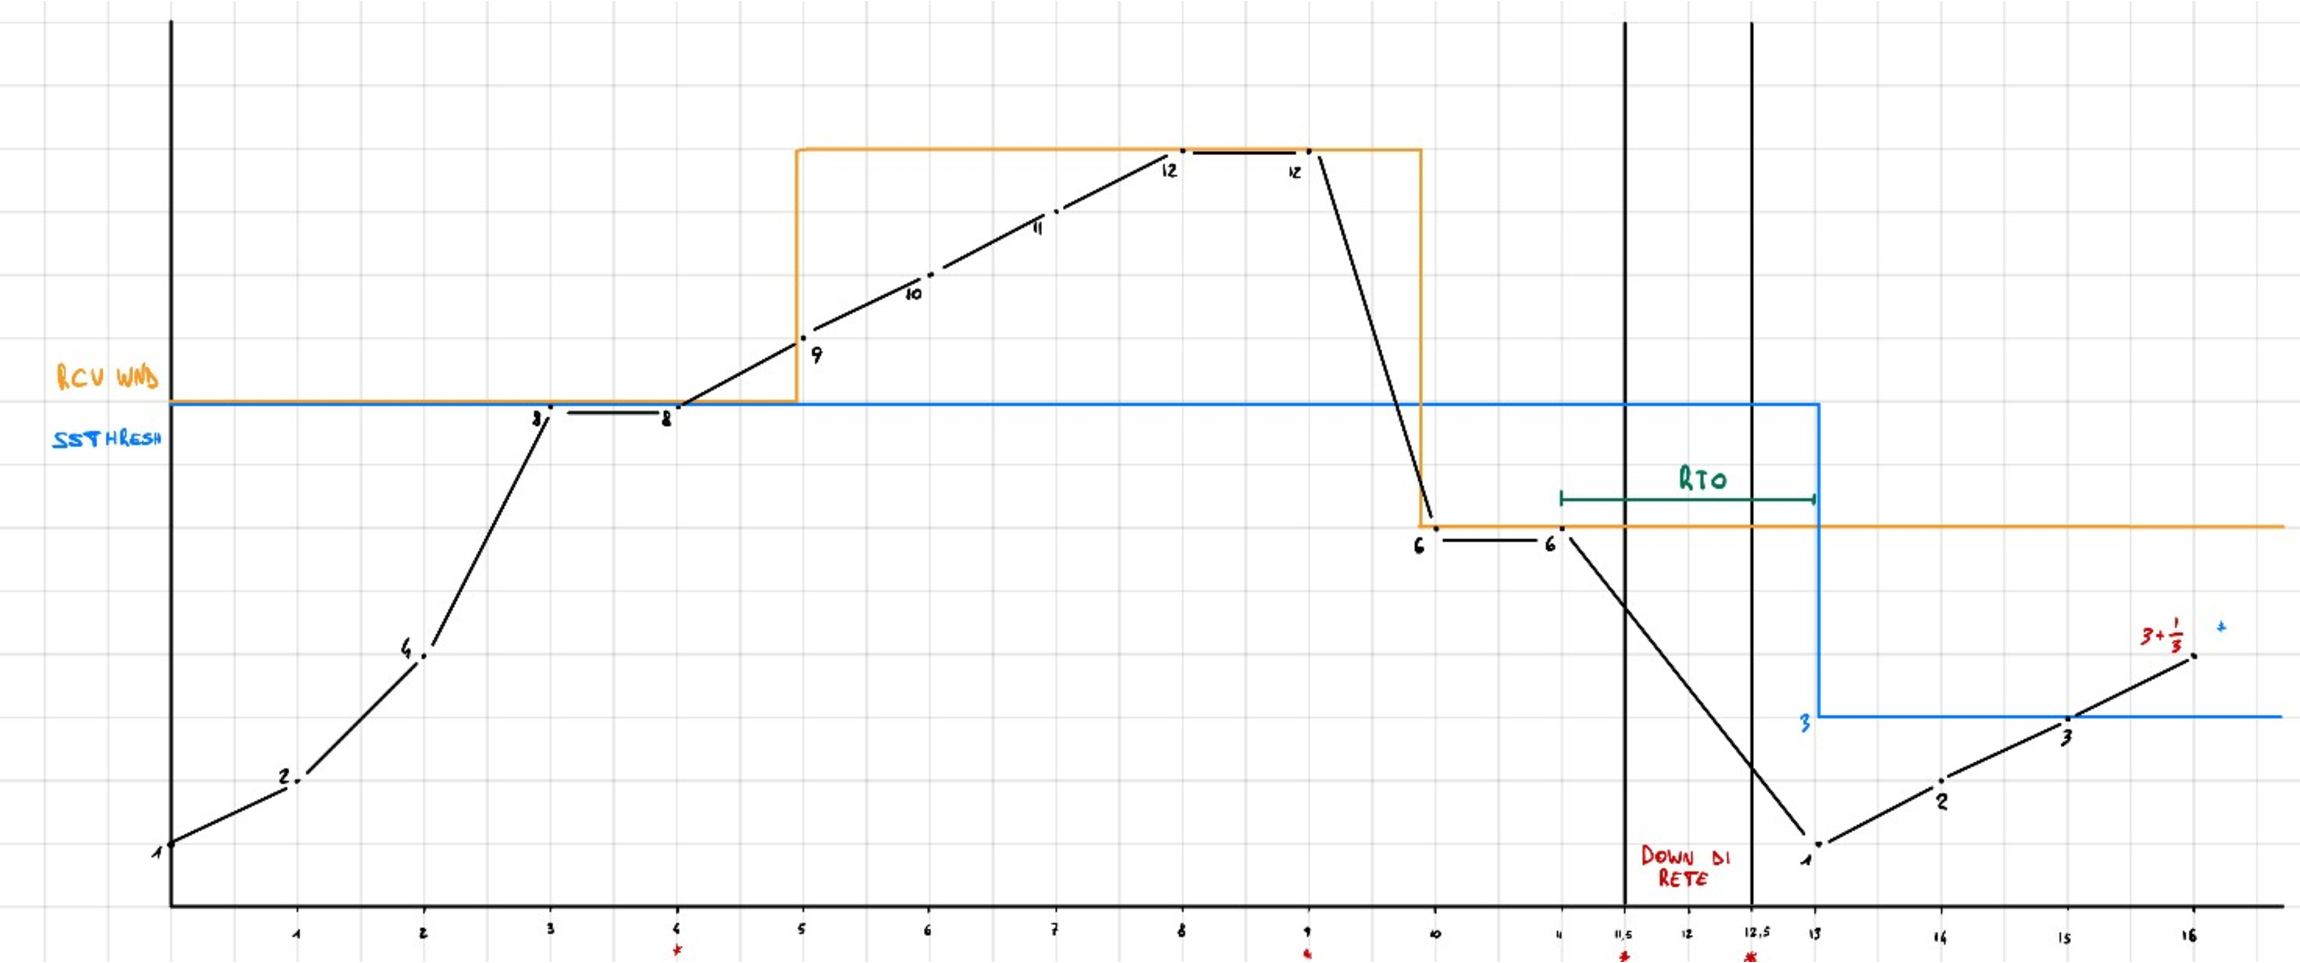
\includegraphics[width=\textwidth]{img/ex4_congestione.pdf}
	\end{figure}

	\noindent
	L’unica osservazione degna di nota riguarda il cambio di \textsf{RCV WND} durante l’invio di pacchetti. Infatti, al tempo $t_{4}$ la destinazione cambia la \textsf{RCV WND} da $8$ a $12$. Questo cambiamento ha effetto solamente una volta ricevuti gli \textsf{ACK} del pacchetto inviato al tempo $t_{4}$. In altre parole, al tempo $t_{4}$ vengono inviati i pacchetti ($8$) e al tempo $t_{5}$ la sorgente viene a conoscenza del cambiamento della \textsf{RCV WND}. A questo punto, seguendo l’algoritmo, i pacchetti da inviare aumentano di $1$ nel tempo finché a $t_{8}$ non raggiungono il massimo.\newline
	
	\noindent
	Ancora una volta, al tempo $t_{9}$ avviene una diminuzione della \textsf{RCV WND}, il mittente si adegua di conseguenza al momento della ricezione dei pacchetti ($12$) inviati.\newline
	
	\noindent
	Il \textbf{\emph{down} di rete} provoca una perdita di pacchetti e la \textsf{SSTHRESH} diventa la metà della \textsf{CWND} precedente, ovvero $6$, diventando quindi $3$.\newline
	
	\noindent
	Infine, la chiusura avviene in modo classico, ovvero:
	\begin{equation*}
		\textsf{CWND}_{old} + \dfrac{\text{\#ack ricevuti}}{\textsf{CWND}_{old}} = 3 + \dfrac{1}{3}
	\end{equation*}
	Il conteggio progressivo:
	\begin{equation*}
		1+2+4+8+8+9+10+11+12+12+6+\cancel{6}+1+2+\cancelto{1}{3}=87
	\end{equation*}\newpage

	\section{Algoritmo di instradamento decentralizzato: \emph{distance-vector}}
	
	\subsection{Definizione}
	
	L'algoritmo \textcolor{Red3}{\textbf{\emph{distance-vector}}} è iterativo, asincrono e distributivo:
	\begin{itemize}
		\item \textbf{Distribuito}. Ciascun nodo riceve parte dell’informazione da uno o più dei suoi vicini direttamente connessi, a cui, dopo aver effettuato il calcolo, restituisce i risultati.
		\item \textbf{Iterativo}. Questo processo si ripete fino a quando non avviene ulteriore scambio informativo tra vicini.
		\item \textbf{Asincrono}. Non richiede che tutti i nodi operino al passo con gli altri.
		\item \textbf{(bonus) Auto-terminante}. Non c’è alcun segnale che il calcolo debba fermarsi, semplicemente si blocca.
	\end{itemize}
	Aspetto interessante, i \textbf{costi minimi} sono correlati dalla nota \textbf{formula di Bellman-Ford}:
	\begin{equation*}
		d_{x}\left(y\right) = \min_{v}\left\{c\left(x,v\right) + d_{v}\left(y\right)\right\}
	\end{equation*}
	In cui $\min_{v}$ riguarda tutti i vicini di $x$.
	
	\subsection{Applicazione}
	
	\textbf{Per applicare l’algoritmo}, viene utilizzata una tabella chiamata \textbf{tabella di routing} in cui vengono mostrate per ogni destinazione: il prossimo salto (\emph{next hop}) e il costo di raggiungimento della destinazione.
	\begin{table}[!htbp]
		\centering
		\begin{tabular}{@{} c c c @{}}
			\toprule
			Destinazione	& Prossimo salto (\emph{next hop})	& Costo \\
			\midrule
			$k$				& $R_{a}$							& $D\left(i,k\right)$ \\
			$w$				& $R_{c}$							& $D\left(i,w\right)$ \\
			\bottomrule
		\end{tabular}
	\end{table}
	Inizialmente, per ogni destinazione se si tratta di un vicino diretto, si utilizza la notazione $D\left(i,v\right) = c\left(i,v\right)$, altrimenti si utilizza la notazione $D\left(i,v\right) = \infty$.\newline
	
	\noindent
	\textbf{Periodicamente} si effettuano cronologicamente queste \textbf{due operazioni}:
	\begin{enumerate}
		\item Il nodo manda ai propri vicini il risultato dell'applicazione dell'algoritmo \emph{Distance Vector};
		\item Grazie ai risultati ottenuti dai vicini al punto precedente, viene aggiornata la tabella di \emph{routing}.
	\end{enumerate}\newpage

	\subsection[Esempio]{\textcolor{Green4}{Esempio}}
	
	Dato il seguente grafo:
	\begin{figure}[!htp]
		\centering
		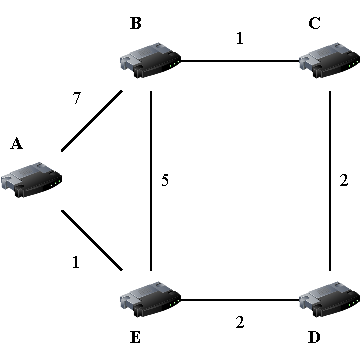
\includegraphics[width=.6\textwidth]{img/eg_grafo.pdf}
	\end{figure}
	
	\noindent
	Si costruiscono le tabelle di \emph{routing} del nodo $A, E$ e $B$.
	\begin{table}[!htbp]
		\centering
		\begin{tabular}{@{} c c c @{}}
			\toprule
			Destinazione	& Prossimo salto (\emph{next hop})	& Costo \\
			\midrule
			$A$				& $-$								& $0$ \\
			$B$				& $B$								& $7$ \\
			$C$				& $-$								& $\infty$ \\
			$D$				& $-$								& $\infty$ \\
			$E$				& $E$								& $1$ \\
			\bottomrule
		\end{tabular}
		\caption{Tabella di \emph{routing} del nodo $A$.}
	\end{table}

	\begin{table}[!htbp]
		\centering
		\begin{tabular}{@{} c c c @{}}
			\toprule
			Destinazione	& Prossimo salto (\emph{next hop})	& Costo \\
			\midrule
			$A$				& $A$								& $1$ \\
			$B$				& $B$								& $5$ \\
			$C$				& $-$								& $\infty$ \\
			$D$				& $D$								& $2$ \\
			$E$				& $-$								& $0$ \\
			\bottomrule
		\end{tabular}
		\caption{Tabella di \emph{routing} del nodo $E$.}
	\end{table}

	\begin{table}[!htbp]
		\centering
		\begin{tabular}{@{} c c c @{}}
			\toprule
			Destinazione	& Prossimo salto (\emph{next hop})	& Costo \\
			\midrule
			$A$				& $A$								& $7$ \\
			$B$				& $-$								& $0$ \\
			$C$				& $C$								& $1$ \\
			$D$				& $-$								& $\infty$ \\
			$E$				& $E$								& $5$ \\
			\bottomrule
		\end{tabular}
		\caption{Tabella di \emph{routing} del nodo $B$.}
	\end{table}\newpage
	
	\noindent
	Nel momento in cui il nodo $A$ riceve il \emph{distance vector} da $B$:
	\begin{gather*}
		D\left(A,B\right) = costo \left(A, \begin{matrix}
			B \\
			E
		\end{matrix}\right) + distanza \left(\begin{matrix}
			B \\
			E
	\end{matrix}, B\right)\\
	\begin{array}{lll}
		\text{Considerando } B & \longrightarrow & C\left(A,B\right) + D\left(B,B\right) = 7 + 0 = 7 \\
		\text{Considerando } E & \longrightarrow & C\left(A,E\right) + D\left(E,B\right) = 1 + \infty = \infty
	\end{array}
	\end{gather*}
	L'equazione scritta viene tradotta nel seguente modo: la distanza dal nodo $A$ al nodo $B$ è data dal costo da $A$ verso il nodo $B$ o il nodo $E$, più la distanza che è stata comunicata dal nodo $B$ o dal nodo $E$, verso $B$. Quindi, sotto l'equazione vengono scritte le casistiche in cui si consideri $B$ o $E$.\newline
	
	\noindent
	Una volta comunicato il \emph{distance vector} ed eseguiti i calcoli, il nodo $A$ \textbf{aggiorna la sua tabella di \emph{routing} inserendo il \underline{valore più piccolo}}. Quindi, in questo caso, $6$ inserendolo nella riga corrispondente a $B$ con relativo \emph{next hop} uguale a $E$.\newline
	
	\noindent
	Nel momento in cui il nodo $A$ riceve il \emph{distance vector} da $C$:
	\begin{gather*}
		D\left(A,C\right) = costo \left(A, \begin{matrix}
			B \\
			E
		\end{matrix}\right) + distanza \left(\begin{matrix}
			B \\
			E
		\end{matrix}, C\right)\\
		\begin{array}{lll}
			\text{Considerando } B & \longrightarrow & C\left(A,B\right) + D\left(B,C\right) = 7 + 1 = 8 \\
			\text{Considerando } E & \longrightarrow & C\left(A,E\right) + D\left(E,C\right) = 1 + \infty = \infty
		\end{array}
	\end{gather*}
	In questo caso, il nodo $A$ aggiornerà la sua tabella di \emph{routing} con il valore $8$ (minimo), inserendolo nella riga corrispondente alla destinazione $C$ e relativo \emph{next hop} pari a $B$.\newpage
	
	\section{Instradamento tra ISP: protocollo BGP}
	
	\subsection{Protocollo BGP}

	Gli \textcolor{Red3}{\textbf{ISP} (\emph{Internet Service Protocol})} utilizzano \textbf{due protocolli} importanti:
	\begin{itemize}
		\item \textbf{Protocollo \underline{OSPF}} (\emph{Open Shortest Path First}), viene utilizzato per \textbf{determinare i percorsi ottimali} per le coppie sorgente-destinazione \textbf{interne ad un sistema autonomo} (utilizzato soprattutto nelle grandi aziende\footnote{Fonte: \href{https://it.wikipedia.org/wiki/Open_Shortest_Path_First}{Wikipedia}}).
		
		\item \textbf{Protocollo \textcolor{Red3}{\textbf{\emph{border gateway protocol}}}} (BGP) è un prtocollo che riesce a determinare i percorsi per le coppie sorgente-destinazione che interessano più sistemi autonomi.
	\end{itemize}
	Attualmente, il protocollo BGP rappresenta l'\textbf{attuale standard dei protocolli di instradamento} dei sistemi autonomi in Internet.\newline
	
	\noindent
	Questo protocollo forse è il più importante dei protocolli di Internet, al pari di IP, in quanto è la colla che tiene insieme le migliaia di ISP che formano Internet. È un \textbf{protocollo} di tipo \textbf{\emph{distance-vector} decentralizzato e asincrono}.\newline
	
	\noindent
	Inoltre, il funzionamento di tale protocollo è molto complesso.\newline
	
	\noindent
	Considerando un Router-Actuator\footnote{È un dispositivo I/O che funge da modulo attuatore che include una funzione di termostato programmabile caldo-freddo} di un ISP, la tabella di routing sarà formata dalle destinazioni che si trovano all'interno dell'ISP, e altre che si trovano all'esterno. Quindi, il protocollo di instradamento inter-AS, che coordina più AS (\emph{autonomous system}\footnote{Fonte: \href{https://it.wikipedia.org/wiki/Sistema_autonomo}{WikipediaIT}, \href{https://en.wikipedia.org/wiki/Autonomous_system_(Internet)}{WikipediaENG}}), gestisce/mantiene le prime, mentre il protocollo BGP le seconde.\newline
	
	\noindent
	Si deduce che il \textbf{\emph{next hop} di una destinazione esterna} sarà il \emph{next hop} che corrisponde al cammino minimo per raggiungere il router di bordo per arrivare a tale rete esterna.\newline
	
	\noindent
	Nel caso in cui \textbf{una destinazione esterna è raggiungibile da più router di bordo}, viene utilizzato il sistema \dquotes{\emph{hot potato routing}}, ovvero viene scelto il gateway più vicino al router che deve instradare il pacchetto.\newpage
	
	\subsection{\textcolor{Red3}{Esercizio - Determinare CIDR e creare subnetting trovando anche indirizzi di broadcast}}
	
	Determinare il blocco \textsf{CIDR} totale sapendo che ci sono 4 reti \textsf{LAN} con i seguenti vincoli::
	\begin{itemize}
		\item \textsf{LAN1} $\longrightarrow 130$ host
		\item \textsf{LAN2} $\longrightarrow 270$ host
		\item \textsf{LAN3} $\longrightarrow 65$ host
		\item \textsf{LAN4} $\longrightarrow 35$ host
	\end{itemize}
	Sapendo che la \textsf{LAN1} contiene l'indirizzo: $46.144.141.41$.\newline
	
	\noindent
	Prima di qualsiasi operazione, si controlla quanti indirizzi necessita ogni \textsf{LAN} e si stabilisce quanti bit servono per raggiungere la richiesta:
	\begin{equation*}
		\begin{array}{lll}
			\textsf{LAN1} & \longrightarrow & 2^{8} = 256 \\
			\textsf{LAN2} & \longrightarrow & 2^{9} = 512 \\
			\textsf{LAN3} & \longrightarrow & 2^{7} = 128 \\
			\textsf{LAN4} & \longrightarrow & 2^{6} = 64
		\end{array}
	\end{equation*}
	Da questi valori si ottiene quanti indirizzi sono necessari per soddisfare tutte le richieste:
	\begin{equation*}
		256 + 512 + 128 + 64 = 960 \approx 2^{10} \emph{ indirizzi}
	\end{equation*}
	Adesso è possibile ottenere il numero di bit che possiede l'indirizzo:
	\begin{equation*}
		2^{32} \div 2^{10} = 2^{22}
	\end{equation*}
	Viene costruito il blocco \textsf{CIDR} della rete partendo dall'indirizzo della \textsf{LAN1} fornito dal testo.\newline
	Per farlo, viene tradotto l'indirizzo in binario:
	\begin{equation*}
		\binaryaddresspointed{00001110}{00010000}{00001101}{00001001}
	\end{equation*}
	Messi a zero i bit del suffisso:
	\begin{equation*}
		\binaryaddress{00001110}{00010000}{000011\boldsymbol{00}}{\boldsymbol{00000000}}
	\end{equation*}
	E ritradotto in decimale per ottenere il blocco \textsf{CIDR}:
	\begin{equation*}
		46.144.140.0/22
	\end{equation*}
	Adesso è possibile creare le sottoreti, quindi si parte diminuendo il suffisso da 10 a 9 ottenendo due indirizzi da assegnare o da scomporre nuovamente:
	\begin{gather*}
		\binaryaddresspointed{00001110}{00010000}{000011\textcolor{Red3}{\boldsymbol{1}}0}{00000000}/23 \rightarrow \textsf{LAN2} \rightarrow 46.144.142.0/23 \\
		\binaryaddress{00001110}{00010000}{000011\textcolor{Red3}{\boldsymbol{0}}0}{00000000}/23
	\end{gather*}
	Si esegue la scomposizione nuovamente, notando che la scelta appena scritta non è stata casuale.\newline
	Infatti, dato che l'indirizzo della \textsf{LAN1} deve essere:
	\begin{equation*}
		\binaryaddresspointed{00001110}{00010000}{00001101}{00001001}
	\end{equation*}
	Il bit non poteva essere 1, perché altrimenti sarebbe stato sbagliato.
	\begin{gather*}
		\binaryaddresspointed{00001110}{00010000}{0000110\textcolor{Red3}{\boldsymbol{1}}}{00000000}/24 \rightarrow \textsf{LAN1} \rightarrow 46.144.141.0/24 \\
		\binaryaddresspointed{00001110}{00010000}{0000110\textcolor{Red3}{\boldsymbol{0}}}{00000000}/24
	\end{gather*}
	Assegnato l'indirizzo alla \textsf{LAN1}, si continua:
	\begin{gather*}
		\binaryaddresspointed{00001110}{00010000}{00001100}{\textcolor{Red3}{\boldsymbol{0}}0000000}/25 \rightarrow \textsf{LAN3} \rightarrow 46.144.140.0/25 \\
		\binaryaddresspointed{00001110}{00010000}{00001100}{\textcolor{Red3}{\boldsymbol{1}}0000000}/25
	\end{gather*}
	Un'ultima volta:
	\begin{gather*}
		\binaryaddresspointed{00001110}{00010000}{00001100}{1\textcolor{Red3}{\boldsymbol{0}}000000}/26 \rightarrow \textsf{LAN4} \rightarrow 46.144.140.128/26 \\
		\binaryaddresspointed{00001110}{00010000}{00001100}{1\textcolor{Red3}{\boldsymbol{1}}000000}/26
	\end{gather*}
	Infine, si ottengono gli indirizzi broadcast mettendo tutti i bit del suffisso ad $1$ e ritraducendo l'indirizzo da binario a decimale. Si omettono i passaggi perché identici a esercizi svolti nei capitoli precedenti:
	\begin{equation*}
		\begin{array}{lll}
			\textsf{LAN1} & \longrightarrow & 46.144.141.255/24 \\
			\textsf{LAN2} & \longrightarrow & 46.144.143.255/23 \\
			\textsf{LAN3} & \longrightarrow & 46.144.140.127/25 \\
			\textsf{LAN4} & \longrightarrow & 46.144.140.191/26
		\end{array}
	\end{equation*}\newpage
	
	\section{DHCP, problema di carenza IP e NAT}
	
	\subsection{DHCP}
	
	Gli indirizzi degli host possono essere configurati manualmente, ma spesso questo compito è svolto utilizzando il \textcolor{Red3}{\textbf{\emph{dynamic host configuration protocol}}} (\textbf{DHCP}). Quest’ultimo \textbf{consente a un host di ottenere un indirizzo IP in modo automatico}, così come di apprendere informazioni aggiuntive, quali la maschera di sottorete, l’indirizzo del router per uscire dalla sottorete (spesso detto router di default o gateway) e l’indirizzo del suo DNS server locale.\newline
	
	\noindent
	Inoltre, il DHCP viene chiamato anche protocollo \textbf{\emph{plug-and-play}} o \textbf{\emph{zero-conf}} (\emph{zero configuration}) grazie alla sua capacità di automatizzare la connessione degli host alla rete.\newline
	
	\noindent
	Per i nuovi host, il protocollo DHCP si articola in quattro punti rappresenta in figura~\ref{DHCP immagine}. Il nome \emph{yiaddrr} (\emph{your Internet address}, il tuo indirizzo Internet) indica l'indirizzo assegnato al client connesso.
	\begin{figure}[!htp]
		\centering
		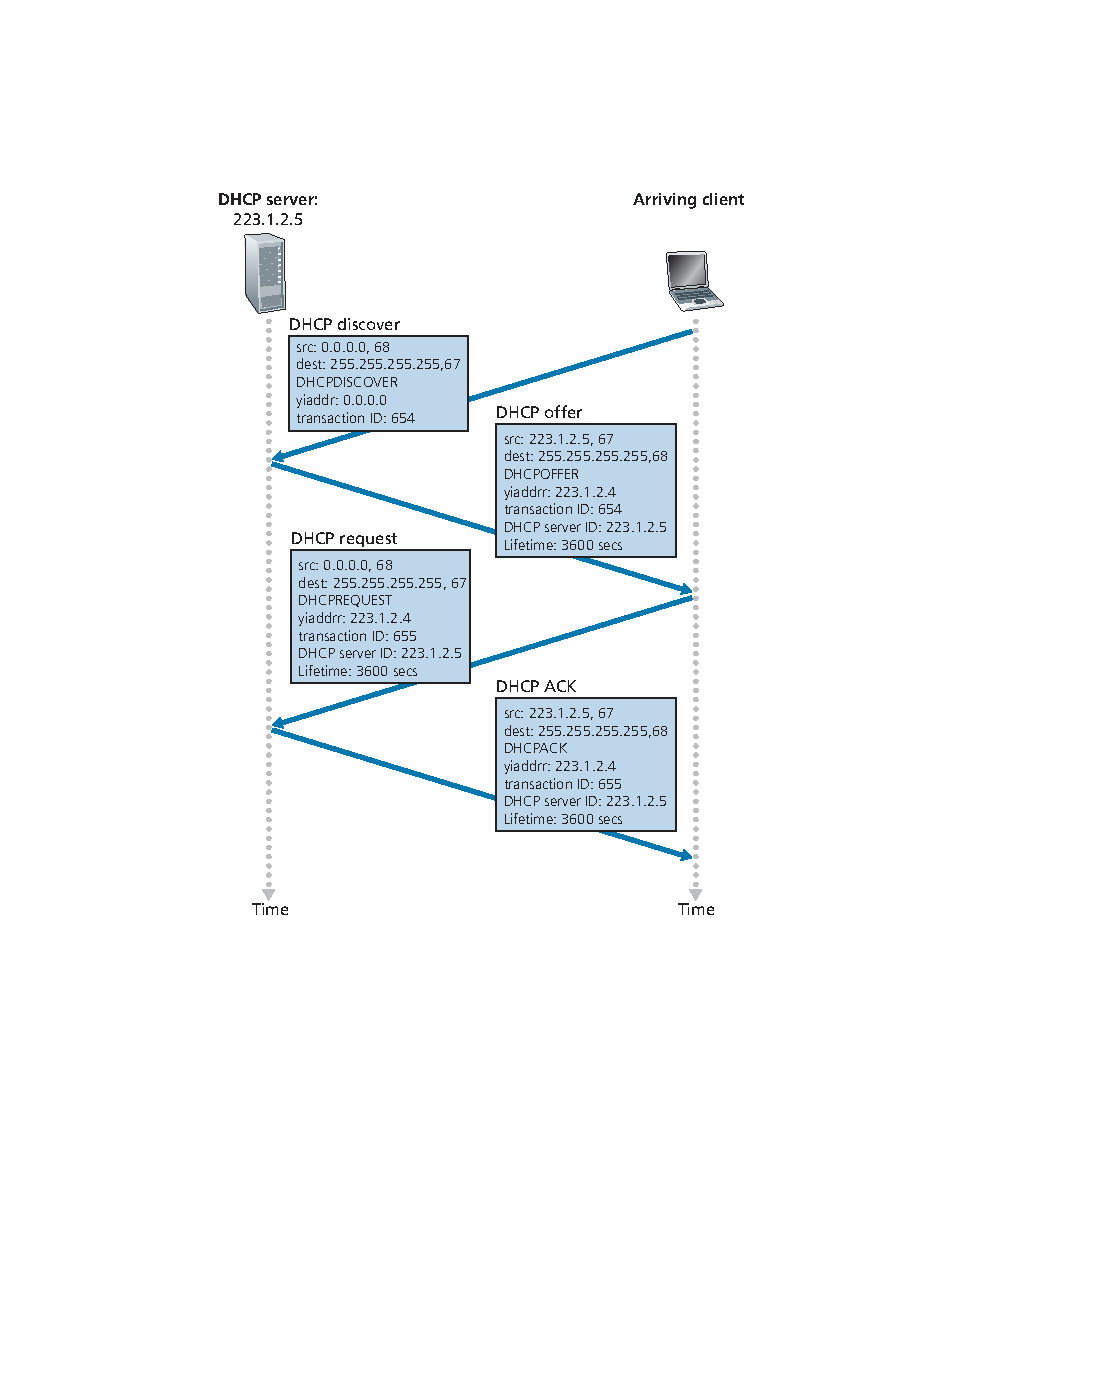
\includegraphics[width=\textwidth]{img/DHCP.pdf}
		\caption{Interazione \emph{client-server} tramite il protocollo DHCP.}\label{DHCP immagine}
	\end{figure}\newpage
	
	\noindent
	I passi eseguiti sono i seguenti:
	\begin{enumerate}
		\item \underline{\textbf{Individuazione del server DHCP (\textcolor{Red3}{DHCP \emph{discover}})}}. L’host collegato ha il compito di trovare il server \textsf{DHCP} con cui interagire. Per farlo \textbf{invia un pacchetto} \textsf{UDP} in modalità \textbf{\emph{broadcast}} a tutti i membri della rete con il messaggio \textsf{DHCP} \emph{discover}, attraverso la porta $67$. Al momento del collegamento, l’host ha un indirizzo IP speciale, cioè $0.0.0.0$ e l’indirizzo \emph{broadcast} che utilizza è $255.255.255.255$
		
		\item \underline{\textbf{Offerta del server DHCP (\textcolor{Red3}{DHCP \emph{offer}})}}. I server interessati (plurale perché in una rete ci possono essere più server!) \textbf{rispondono al messaggio del host} tramite un messaggio di tipo \textsf{DHCP} \emph{offer}, il quale viene \textbf{inviato in \emph{broadcast}} a tutti i nodi della sottorete utilizzando sempre l’indirizzo IP \emph{broadcast} dato che l’host ancora non ha alcun indirizzo IP!\newline
		Il \textbf{server} quando effettua la \textbf{risposta in \emph{broadcast}}, invia:
		\begin{itemize}[label=-]
			\item \textbf{ID} di transazione del messaggio di identificazione ricevuto;
			\item \textbf{Indirizzo IP} proposto al client;
			\item \textbf{Maschera di sottorete};
			\item \textbf{Durata di connessione} (\emph{lease time}) dell'indirizzo IP, cioè il tasso di tempo durante il quale l'indirizzo IP sarà valido.
		\end{itemize}
		
		\item \underline{\textbf{Richiesta DHCP (\textcolor{Red3}{DHCP \emph{request}})}}. L’\textbf{host sceglie} tra le varie offerte dei \textbf{server} e \textbf{risponderà} con un messaggio \textsf{DHCP} \emph{request}, il quale riporta i parametri di configurazione.
		
		\item \underline{\textbf{Conferma DHCP (\textcolor{Red3}{DHCP ACK})}}. Il \textbf{server risponde} al messaggio di richiesta \textsf{DHCP} con un messaggio \textsf{DHCP ACK}, che conferma i parametri richiesti.
	\end{enumerate}

	\subsection{Carenza degli indirizzi IP}
	
	Con gli IP a $32$ bit è possibile creare al massimo 4 miliardi di indirizzi IP. È evidente come sia un problema ai giorni nostri, dato che nel mondo siamo più di 8 miliardi. Esistono due possibili soluzioni a questa carenza:
	\begin{enumerate}
		\item Cambiare il protocollo IP da IPv4 al protocollo IPv6;
		\item Introdurre classi di indirizzi privati.
	\end{enumerate}
	La prima soluzione è un po' utopistica ora come ora poiché cambiare il protocollo vorrebbe dire cambiare le infrastrutture di programmazione create molti anni fa e attualmente funzionanti. La seconda, invece, è quella attuale.\newline
	
	\noindent
	Quindi, attualmente esistono \textbf{due tipi di indirizzi IP}:
	\begin{itemize}
		\item \textcolor{Red3}{\textbf{Pubblici}}, sono unici, quindi non esistono doppioni;
		\item \textcolor{Red3}{\textbf{Privati}}, usati nelle rete locali, unici quindi all'interno di una rete locale. Tuttavia, non hanno la possibilità di essere esposti al mondo di Internet (indirizzi più comuni: $10.0.0.0/8$, $172.16.0.0/12$, $192.168.0.0/16$, $169.254.0.0/16$).
	\end{itemize}
	
	\subsection{NAT}
	
	Pensandoci bene, gli indirizzi IP privati \textbf{non possono comunicare all'esterno di una rete locale}. Dunque, sorge spontanea una domanda: qual è il loro scopo?\newline
	Per rispondere, si introduce il \textcolor{Red3}{\textbf{\emph{Network Address Translation}}}.
	\begin{figure}[!htp]
		\centering
		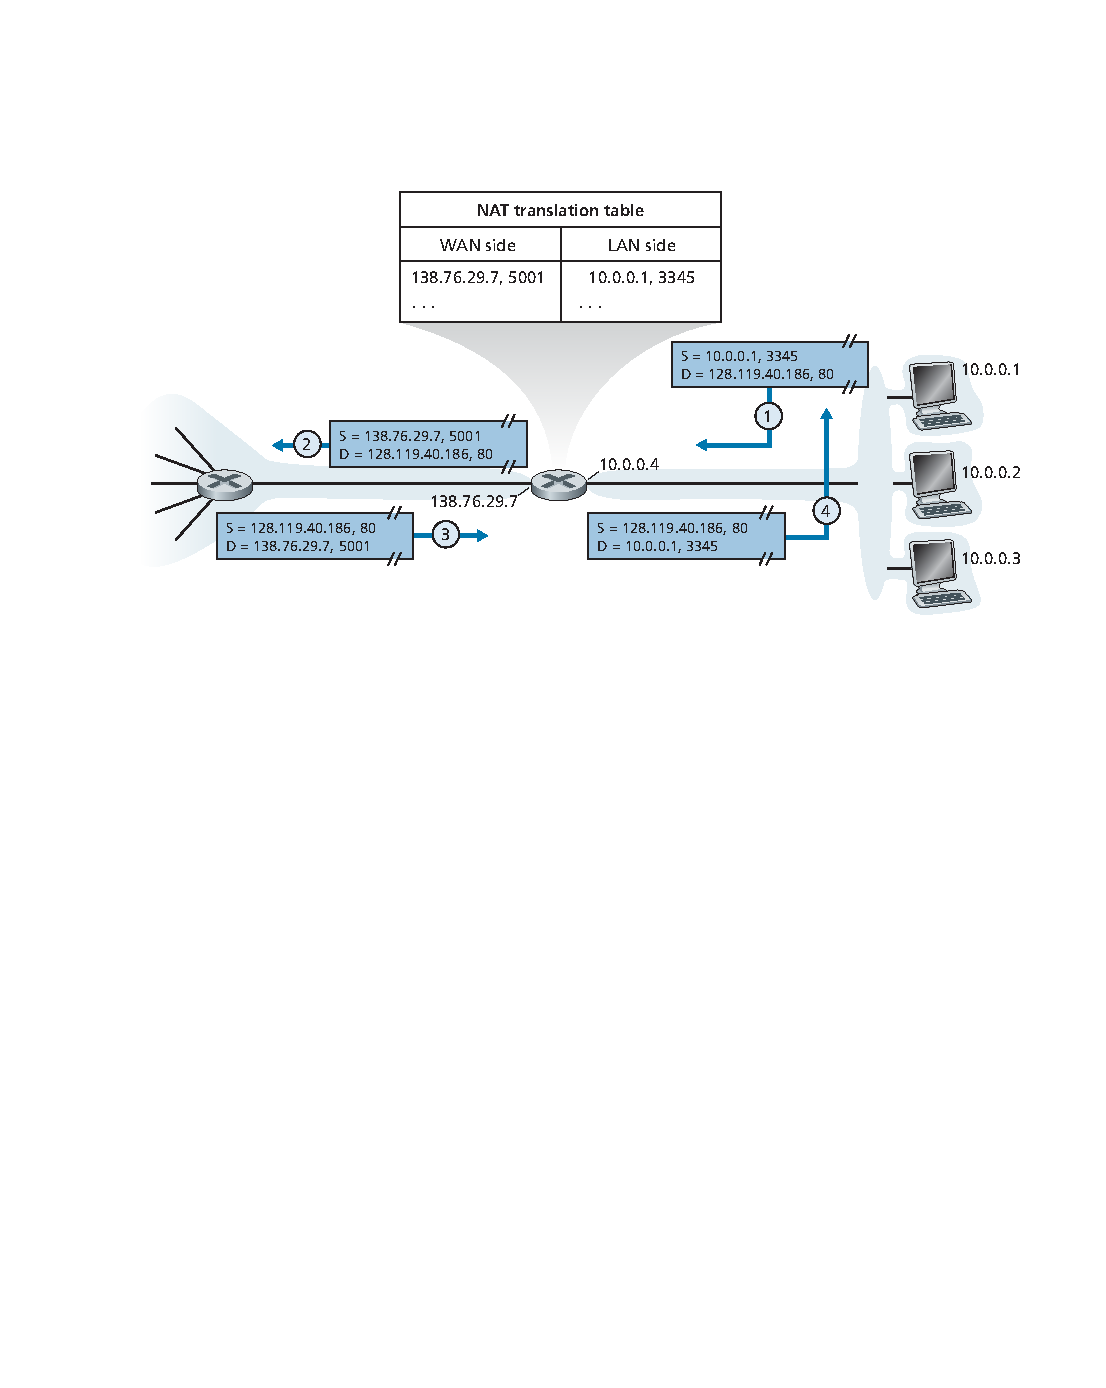
\includegraphics[width=\textwidth]{img/NAT.pdf}
		\caption{Funzionamento di \textsf{NAT} (\emph{Network Address Translation}).}
	\end{figure}

	\noindent
	L’\underline{\textbf{obbiettivo}} del \textsf{NAT} è quello di \textbf{consentire a gli indirizzi IP privati di comunicare tramite Internet}. Ovviamente, questo sistema consente di risparmiare moltissimi indirizzi IP e di salvaguardare anche la sicurezza.\newline
	
	\noindent
	I router abilitati al \textsf{NAT} non appaiono come \textbf{router} al mondo esterno, ma si \textbf{comportano come un \underline{unico} dispositivo con un \underline{unico} indirizzo IP}. In figura tutto il traffico che lascia il router domestico verso Internet ha l’indirizzo IP di origine $138.76.29.7$ e tutto il traffico in entrata deve avere lo stesso indirizzo come destinazione.\newline
	
	\noindent
	Se tutti i datagrammi in arrivo al router \textsf{NAT} della rete geografica hanno lo stesso indirizzo IP di destinazione, allora come capisce il router ha quale host interno inoltrare il datagramma? Viene \textbf{utilizza una tabella di traduzione \textsf{NAT}} (\textsf{NAT} \emph{translation table}) nel router \textsf{NAT} e vengono incluse delle righe nella tabella contenenti il numero di porta oltre che gli indirizzi IP.\newline
	
	\noindent
	Quindi, il router scrive l’indirizzo di destinazione del datagramma e il suo numero di porta di destinazione e inoltra il datagramma nella rete domestica.\newpage
	
	\section{Formato dei datagrammi IPv6}
	
	\subsection{Datagramma IPv6}
	
	Qui di seguito viene riportato il formato di un \textcolor{Red3}{\textbf{datagramma di un protocollo IP versione 6}} (IPv6). La mancata descrizione di alcuni campi non è un errore. Data la somiglianza con la versione 4, si rimanda al capitolo~\ref{ipv4} a pagina~\pageref{ipv4}.
	\begin{figure}[!htp]
		\centering
		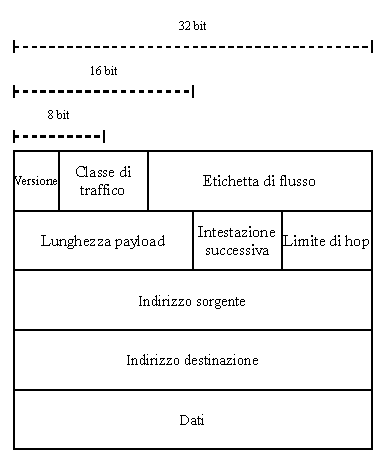
\includegraphics[width=.85\textwidth]{img/datagrammi_ipv6.pdf}
		\caption{Formato dei datagrammi nella versione IPv6.}
	\end{figure}

	\noindent
	I \textbf{\underline{cambiamenti} più significativi} e i campi identici sono:
	\begin{itemize}[label=\ding{51}]
		\item \textbf{Indirizzamento esteso}. La dimensione dell'indirizzo IP passa da 32 bit a 128 bit, così che gli indirizzi IP diventino praticamente inesauribili ($2^{128} = 340$ undecillion, $340$ trilioni di trilioni di trilioni).
		
		\item \textbf{Intestazione ottimizzata di 40 byte}. L'intestazione pari a 40 byte, lunghezza fissa, consente una più rapida elaborazione dei datagrammi IP, mentre una nuova codifica delle opzioni ne consente l’elaborazione più flessibile.
		
		\item \textbf{Etichettatura dei flussi}. Un \textbf{flusso} in un IPv6 è una sorta di \textbf{etichettatura effettuata ai pacchetti per i quali il mittente richiede una gestione speciale}, come una qualità di servizio diversa da quella di default o un servizio in tempo reale.
	\end{itemize}
	Le \textbf{\underline{principali differenze} con la versione 4} (IPv4) sono:
	\begin{itemize}
		\item \textbf{Versione}. Campo da 4 bit che identifica il numero di versione IP, che per IPv6 è uguale a 6.
		
		\item \textbf{Classe di traffico}. Campo da 8 bit, simile al campo \textsf{TOS} in IPv4. Viene usato per attribuire proprietà a determinati datagrammi all'interno di un flusso.
		
		\item \textbf{Etichetta di flusso}. Campo da 20 bit utilizzato per identificare un flusso di datagrammi.
		
		\item \textbf{Lunghezza del payload}. Questo valore a 16 bit viene considerato senza segno e indica il numero di byte nel datagramma IPv6 che seguono l'intestazione a lunghezza fissa di 40 byte.
		
		\item \textbf{Intestazione successiva}. L'intestazione del datagramma è formato da 40 byte. Tuttavia, è possibile aggiungere altre informazioni utilizzando il campo \emph{next header} (intestazione successiva). Esso ha un doppio significato:
		\begin{enumerate}
			\item Se non è presente un'estensione e l'intestazione rimane a 40 byte, allora il campo identifica il protocollo a cui verranno consegnati i contenuti (campo dati) del datagramma, per esempio \textsf{UDP} o \textsf{TCP}.
			
			\item Se è presente un'estensione (\emph{extension header}) e l'intestazione supera i 40 byte, allora il campo identifica il tipo di \textbf{\emph{extension header}}\footnote{L'\emph{extension header} è formato da due campi obbligatori ed i restanti liberi. Il primo campo (8 bit) rappresenta \emph{next header} che ha lo stesso funzionamento già descritto e il secondo (8 bit) rappresenta \emph{header length} che identifica (valore) quanto è lunga l'estensione.}
		\end{enumerate}
		
		\item \textbf{Limite di hop}. Viene decrementato di 1 da ogni router che inoltra il datagramma. Una volta a zero viene eliminato il datagramma.
		
		\item \textbf{Indirizzi sorgente e destinazione}. I diversi formati degli indirizzi IPv6 a 128 bit sono descritti nell'RFC 4291.
		
		\item \textbf{Dati}. È il \emph{payload} che viene passato al protocollo specificato nel campo di \dquotes{intestazione successiva} quando il datagramma IPv6 raggiunge una destinazione.
	\end{itemize}\newpage
	Inoltre, rispetto alla versione IPv4 sono stati \textbf{\underline{eliminati}}:
	\begin{itemize}[label=\ding{55}]
		\item \textbf{Frammentazione/riassemblaggio}. IPv6 non consente queste operazioni ai router intermedi, ma le effettuano solamente la sorgente o destinazione, quindi le periferiche che sono \underline{molto più rapide} più rapide. Nel caso di una dimensione eccessiva, viene inviato un errore al mittente.
		
		\item \textbf{Checksum dell’intestazione}. I protocolli Internet a livello di trasporto (\textsf{UDP} e \textsf{TCP}) e di collegamento (Ethernet) calcolano un loro \emph{checksum}. I progettisti hanno dunque pensato che fosse una funzionalità ridondante. Infatti, nel IPv4, ogni router deve ricalcolare il \emph{checksum} dell’intestazione.
		
		\item \textbf{Opzioni}. Grazie all’eliminazione di questo campo, la lunghezza dell’intestazione IP è fissata a 40 byte.
	\end{itemize}
	Infine, per rappresentare gli indirizzi con la versione IPv6 si utilizza la \textbf{notazione esadecimale}, la quale è molto più compatta della decimale. Quindi, dato che ci sono 128 bit, vengono formati 8 gruppi da 16 bit. Ogni gruppo viene rappresentato con 4 semplici cifre esadecimali ($4$ bit $\times 4$ cifre $ = 16$ bit). Per esempio $69\mathrm{DC} : 8864 : \mathrm{FFFF} : 0000 : \cdots$.\newpage
	
	\subsection{\textcolor{Red3}{Esercizio sul controllo della congestione TCP}}
	
	L’applicazione A deve trasferire all'applicazione B $77'500$ Byte. La connessione è già stata instaurata. I dati disponibili sono:
	\begin{itemize}
		\item $\textsf{MSS} = 1'250$ Byte
		\item $\textsf{RCV WND} = 10'000$ Byte costante
		\item $\textsf{SSTHRESH} = \textsf{RCV WND}$ iniziale
		\item $\textsf{RTT} = 1$ secondo costante
		\item $\textsf{RTO} = \textsf{RTT} \times 2$ e raddoppia in caso di perdite consecutive
	\end{itemize}
	Infine, negli intervalli aperti $8.00 - 10.00$ e $13.5 - 14.5$ è presente un \emph{down} di rete. Inoltre:
	\begin{itemize}
		\item A partire da $t_{A} > 4.0$ la destinazione annuncia una $\textsf{RCV WND} = 17'500$ Byte;
		\item A partire da $t_{B} > 8.0$ la destinazione annuncia una $\textsf{RCV WND} = 12'500$ Byte.
	\end{itemize}
	
	\noindent
	Il \textbf{primo passo} per risolvere l'esercizio è la numerazione dei segmenti. Per farlo basta prendere il numero dei Byte da trasferire e dividere il valore per la \textsf{MSS}:
	\begin{equation*}
		\textbf{Numero di segmenti da inviare } \rightarrow 77'500 \div 1'250 = 62 \emph{ segmenti}
	\end{equation*}
	Prima di passare al secondo passaggio e osservare il numero di segmenti da inviare, è necessario ottenere il valore della \textsf{RCV WND} (finestra massima di ricezione) per avere conseguentemente anche la \textsf{CWND}. Essa è possibile calcolarla facendo una semplice divisione tra il numero di Byte della \textsf{RCV WND} e della \textsf{MSS}:
	\begin{equation*}
		\begin{array}{lll}
			\textbf{\textsf{RCV WND}} & \rightarrow & 10'000 \div 1'250 = 8 \emph{ segmenti} \\
			\textbf{\textsf{RCV WND}}\text{ al tempo }t_{4} & \rightarrow & 17'500 \div 1'250 = 14 \emph{ segmenti} \\
			\textbf{\textsf{RCV WND}}\text{ al tempo }t_{8} & \rightarrow & 12'500 \div 1'250 = 10 \emph{ segmenti}
		\end{array}
	\end{equation*}
	E la \textsf{SSTHRESH}, come scritto nei dati del testo dell'esercizio, è uguale alla \emph{receive window}:
	\begin{equation*}
		\textsf{\textbf{SSTHRESH}} \rightarrow 8 \emph{ segmenti}
	\end{equation*}\newpage
	
	\noindent
	Il \textbf{secondo passo} necessita di uno schema. Esso ha nell’asse delle ascisse ($x$) il tempo e nell’asse delle ordinate ($y$) la \textsf{CWND}.
	\begin{figure}[!htp]
		\centering
		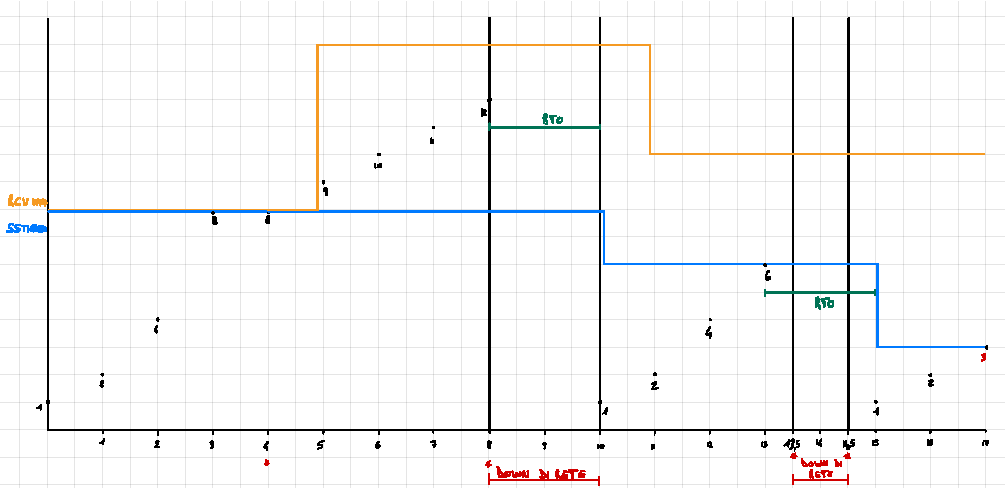
\includegraphics[width=\textwidth]{img/ex5_congestione.pdf}
	\end{figure}
	
	\noindent
	L’unica osservazione da effettuare è il cambiamento della \textsf{RCV WND}. Infatti, quest’ultima, al tempo $t_{8}$ sarebbe dovuta diventare uguale a $10$. Tuttavia, a causa del down di rete, il destinatario non è riuscito a comunicare il cambio di \textsf{RCV WND} al mittente.\newline
	
	\noindent
	La comunicazione è dunque avvenuta solamente quando il mittente, allo scadere del \textsf{RTO} al tempo $t_{10}$, ha inviato $1$ segmento al destinatario, ricevendo sia il relativo \textsf{ACK} che l’aggiornamento.\newline
	
	\noindent
	La chiusura avviene con il valore $3$ poiché viene effettuato il confronto del valore minimo tra:
	\begin{equation*}
		\min\left\{\textsf{CWND}_{old} + \text{\#ack ricevuti}, \textsf{RCV WND}, \textsf{SSTHRESH}\right\}
	\end{equation*}
	Quindi:
	\begin{equation*}
		\min\left\{2+1,10,3\right\}
	\end{equation*}
	Il conteggio progressivo è il seguente:
	\begin{equation*}
		1+2+4+8+8+9+10+11+ \cancel{12} +1+2+4+ \cancel{6} +1+ \cancelto{1}{2} =62
	\end{equation*}\newpage
	
	\section{Livello logico (o di collegamento)}
	
	\subsection{Premessa}
	
	Prima di introdurre questo nuovo livello, è necessario conoscere dei termini utili:
	\begin{itemize}[label=-]
		\item Un \textbf{nodo} è qualunque dispositivo che opera a livello logico, o di collegamento (livello 2);
		
		\item I \textbf{collegamenti} (\emph{link}) sono canali di comunicazione, che collegano nodi adiacenti lungo un cammino. Quindi, i datagrammi che devono essere trasferiti da un host sorgente a un host di destinazione, devono essere trasportati lungo ciascun collegamento nel percorso da un estremo all’altro.
		
		\item Un \textbf{frame del livello di collegamento} (\emph{link-layer frame}) viene creato da un nodo trasmittente quando incapsula il datagramma. Questo accade su ogni collegamento e successivamente lo trasmette lungo il collegamento stesso.
	\end{itemize}

	\subsection{Definizione}

	Al \textcolor{Red3}{\textbf{livello logico}} l'\textbf{obbiettivo principale} è quello di gestire le problematiche associate alla trasmissione sul singolo \emph{hop}. Inoltre, Esistono altri tipi di servizi che vengono offerti dai vari protocolli:
	\begin{itemize}
		\item \textcolor{Red3}{\textbf{Framing}}. Quasi tutti i protocolli incapsulano i datagrammi del livello di rete all'interno di un frame a livello logico (o di collegamento), prima di trasmetterlo;
		
		\item \textcolor{Red3}{\textbf{Accesso al collegamento}}. Un protocollo che controlla l'accesso al mezzo trasmittivo (MAC, \emph{medium access control}) e specifica le regole con cui immette i frame nel collegamento. Esistono dei casi in cui vari nodi condividono un singolo canale broadcast e qui nasce il \textbf{problema degli accessi multipli} trattato nel prossimo capitolo.
		
		\item \textcolor{Red3}{\textbf{Consegna affidabile}}. I protocolli a livello logico (o di collegamento) che forniscono un servizio di consegna affidabile garantiscono il trasporto senza errori di ciascun datagramma.
		
		\item \textcolor{Red3}{\textbf{Rilevazione e correzione degli errori}}. Il nodo ricevente può decidere, erroneamente, che un bit in un frame sia $0$ quando questo era stato trasmesso come $1$, e viceversa. Gli errori di bit sono causati dall’attenuazione di segnale e dai disturbi elettromagnetici. Quindi, molti protocolli del livello logico (o di collegamento), forniscono un meccanismo per rivelarne la presenza.
	\end{itemize}
	Infine, il livello logico (o di collegamento) viene implementato fisicamente, cioè \emph{hardware}, e logicamente, cioè \emph{software}. La figura mostra una tipica architettura di un host.\newpage
	
	\begin{figure}[!htp]
		\centering
		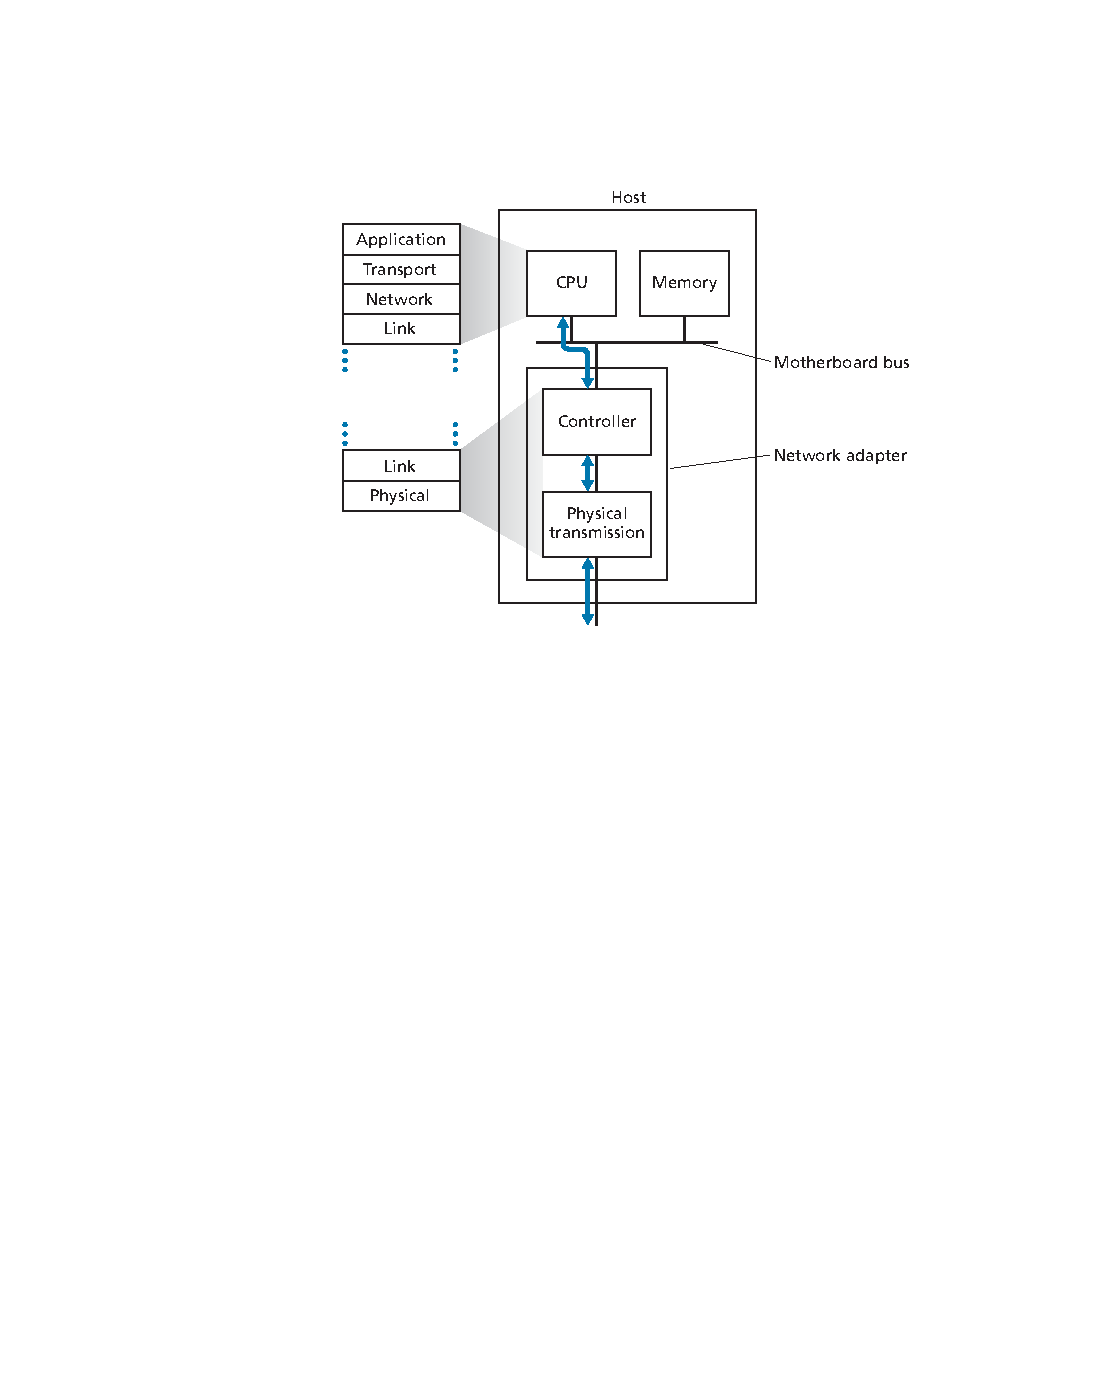
\includegraphics[width=\textwidth]{img/architettura_host.pdf}
		\caption{Tipica architettura di un host. A fianco si possono vedere i vari livelli.}
	\end{figure}
	
	\noindent
	Per un dato collegamento, il protocollo del livello logico (o di collegamento) è sostanzialmente realizzato da un \textbf{adattatore di rete} (\emph{network adapter}), noto anche come scheda di rete (NIC, \emph{network interface card}).\newpage
	
	\subsection{\textcolor{Red3}{Esercizio - Determinare CIDR e creare subnetting}}
	
	Determinare il blocco \textsf{CIDR} totale sapendo che ci sono 3 reti \textsf{LAN} con i seguenti vincoli::
	\begin{itemize}
		\item \textsf{LAN1} $\longrightarrow 400$ host
		\item \textsf{LAN2} $\longrightarrow 300$ host
		\item \textsf{LAN3} $\longrightarrow 1200$ host
	\end{itemize}
	Sapendo che la \textsf{LAN1} contiene l'indirizzo: $178.242.85.168$.\newline
	
	\noindent
	Prima di qualsiasi operazione, si controlla quanti indirizzi necessita ogni \textsf{LAN} e si stabilisce quanti bit servono per raggiungere la richiesta:
	\begin{equation*}
		\begin{array}{lll}
			\textsf{LAN1} & \longrightarrow & 2^{9} = 512 \\
			\textsf{LAN2} & \longrightarrow & 2^{9} = 512 \\
			\textsf{LAN3} & \longrightarrow & 2^{11} = 2048 
		\end{array}
	\end{equation*}
	Da questi valori si ottiene quanti indirizzi sono necessari per soddisfare tutte le richieste:
	\begin{equation*}
		512 + 512 + 2048 = 3072 \approx 2^{12} \emph{ indirizzi}
	\end{equation*}
	Adesso è possibile ottenere il numero di bit che possiede l'indirizzo:
	\begin{equation*}
		2^{32} \div 2^{12} = 2^{20}
	\end{equation*}
	Viene costruito il blocco \textsf{CIDR} della rete partendo dall'indirizzo della \textsf{LAN1} fornito dal testo.\newline
	Per farlo, viene tradotto l'indirizzo in binario:
	\begin{equation*}
		\binaryaddresspointed{10110010}{11110010}{01010101}{10101000}
	\end{equation*}
	Messi a zero i bit del suffisso:
	\begin{equation*}
		\binaryaddress{10110010}{11110010}{0101\boldsymbol{0000}}{\boldsymbol{00000000}}
	\end{equation*}
	E ritradotto in decimale per ottenere il blocco \textsf{CIDR}:
	\begin{equation*}
		178.242.80.0/20
	\end{equation*}
	Adesso è possibile creare le sottoreti, quindi si parte diminuendo il suffisso da $12$ a $11$ ottenendo due indirizzi da assegnare o da scomporre nuovamente:
	\begin{gather*}
		\binaryaddresspointed{10110010}{11110010}{0101\textcolor{Red3}{\boldsymbol{0}}000}{00000000}/21 \\
		\binaryaddress{10110010}{11110010}{0101\textcolor{Red3}{\boldsymbol{1}}000}{00000000}/21 \rightarrow \textsf{LAN3} \rightarrow 178.242.88.0/21
	\end{gather*}
	Si esegue la scomposizione nuovamente, notando che la scelta appena scritta non è stata casuale.\newline
	Infatti, dato che l'indirizzo della \textsf{LAN1} deve essere:
	\begin{equation*}
		\binaryaddresspointed{10110010}{11110010}{01010101}{10101000}
	\end{equation*}
	Il bit non poteva essere $1$, perché altrimenti sarebbe stato sbagliato.
	\begin{gather*}
		\binaryaddresspointed{10110010}{11110010}{01010\textcolor{Red3}{\boldsymbol{0}}00}{00000000}/22 \\
		\binaryaddresspointed{10110010}{11110010}{01010\textcolor{Red3}{\boldsymbol{1}}00}{00000000}/22
	\end{gather*}
	Il primo indirizzo viene lasciato libero e si continua dunque con il \emph{subnetting} sfruttando il secondo indirizzo:
	\begin{equation*}
		\begin{array}{lllll}
			\binaryaddresspointed{10110010}{11110010}{010101\textcolor{Red3}{\boldsymbol{0}}0}{00000000}/23 & \rightarrow & \textsf{LAN1} & \rightarrow & 178.242.84.0/23 \\
			\binaryaddresspointed{10110010}{11110010}{010101\textcolor{Red3}{\boldsymbol{1}}0}{00000000}/23 & \rightarrow & \textsf{LAN2} & \rightarrow & 178.242.86.0/23
		\end{array}
	\end{equation*}
\end{document}